\documentclass[12pt]{article}\usepackage[]{graphicx}\usepackage[]{color}
%% maxwidth is the original width if it is less than linewidth
%% otherwise use linewidth (to make sure the graphics do not exceed the margin)
\makeatletter
\def\maxwidth{ %
  \ifdim\Gin@nat@width>\linewidth
    \linewidth
  \else
    \Gin@nat@width
  \fi
}
\makeatother

\definecolor{fgcolor}{rgb}{0.345, 0.345, 0.345}
\newcommand{\hlnum}[1]{\textcolor[rgb]{0.686,0.059,0.569}{#1}}%
\newcommand{\hlstr}[1]{\textcolor[rgb]{0.192,0.494,0.8}{#1}}%
\newcommand{\hlcom}[1]{\textcolor[rgb]{0.678,0.584,0.686}{\textit{#1}}}%
\newcommand{\hlopt}[1]{\textcolor[rgb]{0,0,0}{#1}}%
\newcommand{\hlstd}[1]{\textcolor[rgb]{0.345,0.345,0.345}{#1}}%
\newcommand{\hlkwa}[1]{\textcolor[rgb]{0.161,0.373,0.58}{\textbf{#1}}}%
\newcommand{\hlkwb}[1]{\textcolor[rgb]{0.69,0.353,0.396}{#1}}%
\newcommand{\hlkwc}[1]{\textcolor[rgb]{0.333,0.667,0.333}{#1}}%
\newcommand{\hlkwd}[1]{\textcolor[rgb]{0.737,0.353,0.396}{\textbf{#1}}}%

\usepackage{framed}
\makeatletter
\newenvironment{kframe}{%
 \def\at@end@of@kframe{}%
 \ifinner\ifhmode%
  \def\at@end@of@kframe{\end{minipage}}%
  \begin{minipage}{\columnwidth}%
 \fi\fi%
 \def\FrameCommand##1{\hskip\@totalleftmargin \hskip-\fboxsep
 \colorbox{shadecolor}{##1}\hskip-\fboxsep
     % There is no \\@totalrightmargin, so:
     \hskip-\linewidth \hskip-\@totalleftmargin \hskip\columnwidth}%
 \MakeFramed {\advance\hsize-\width
   \@totalleftmargin\z@ \linewidth\hsize
   \@setminipage}}%
 {\par\unskip\endMakeFramed%
 \at@end@of@kframe}
\makeatother

\definecolor{shadecolor}{rgb}{.97, .97, .97}
\definecolor{messagecolor}{rgb}{0, 0, 0}
\definecolor{warningcolor}{rgb}{1, 0, 1}
\definecolor{errorcolor}{rgb}{1, 0, 0}
\newenvironment{knitrout}{}{} % an empty environment to be redefined in TeX

\usepackage{alltt}
\usepackage[utf8]{inputenc}
\usepackage{graphicx}
\usepackage{color, colortbl}
\definecolor{blue1}{RGB}{0, 102, 204}
\usepackage[colorlinks = true, linkcolor = blue, citecolor = blue, urlcolor = blue]{hyperref}
\usepackage{array}
\usepackage[english]{babel}
\usepackage{amsfonts}
\usepackage{url}
\usepackage{fullpage}
\usepackage{pdflscape}
\usepackage{bm}
\usepackage[margin = 1.5cm]{geometry}
\usepackage[affil-it]{authblk}
\usepackage{hyperref}
\usepackage{multirow}
\usepackage[labelfont = bf]{caption}
\usepackage{amsmath}

\setlength{\doublerulesep}{0pt}

%Numbering figures
\numberwithin{figure}{section}

\title{Appendix S9: results after Qiime Open ref clustering}
\author{Adrien Taudiere\thanks{\texttt{adrien.taudiere@cefe.cnrs.fr}}}

\affil{{\footnotesize CEFE - Centre d'Ecologie Fonctionnelle et Evolutive, Montpellier: France}}

\date{\today}

\sloppy
\hyphenpenalty 10000



%%%%%%% Allow a subsubsub section  %%%%%%%%%
%%%%%%%%%%%%%%%%%%%%%%%%%%%%%%%%%%%%%%%%%%%%%%%%%%
\setcounter{secnumdepth}{4}
\setcounter{tocdepth}{4}
\makeatletter
\newcounter {subsubsubsection}[subsubsection]
\renewcommand\thesubsubsubsection{\thesubsubsection .\@arabic\c@subsubsubsection}
\newcommand\subsubsubsection{\@startsection{subsubsubsection}{4}{\z@}%
          {-3.25ex\@plus -1ex \@minus -.2ex}%
          {1.5ex \@plus .2ex}%
          {\normalfont\normalsize\bfseries}}
\renewcommand\paragraph{\@startsection{paragraph}{5}{\z@}%
         {3.25ex \@plus1ex \@minus.2ex}%
         {-1em}%
         {\normalfont\normalsize\bfseries}}
\renewcommand\subparagraph{\@startsection{subparagraph}{6}{\parindent}%
          {3.25ex \@plus1ex \@minus .2ex}%
          {-1em}%
          {\normalfont\normalsize\bfseries}}
\newcommand*\l@subsubsubsection{\@dottedtocline{4}{10.0em}{4.1em}}
\renewcommand*\l@paragraph{\@dottedtocline{5}{10em}{5em}}
\renewcommand*\l@subparagraph{\@dottedtocline{6}{12em}{6em}}
\newcommand*{\subsubsubsectionmark}[1]{}
\makeatother

\usepackage{hyperref}

\makeatletter
\def\toclevel@subsubsubsection{4}
\def\toclevel@paragraph{5}
\def\toclevel@subparagraph{6}
\makeatother


\definecolor{ligthgray}{RGB}{218, 218, 218}

%%%%%%%%%%%%%%%%%%%%%%%%%%%%%%%%%%%%%%%%%%%%%%%%%%
%%%%%%%%%%%%%%%%%%%%%%%%%%%%%%%%%%%%%%%%%%%%%%%%%%
%%%%%%%%%%%%%%%%%%%%%%%%%%%%%%%%%%%%%%%%%%%%%%%%%%
\IfFileExists{upquote.sty}{\usepackage{upquote}}{}
\begin{document}
\selectlanguage{english}






\maketitle

\vfill
\begin{center}
\textbf{To set the filter parameter, see directly section 'Choice of filter parameters'~\ref{section:filter}.}

\textbf{Don't forgot to set working directory.}
\end{center}

\newpage
\tableofcontents
\newpage


\section{Introduction}

This supplementary material presents the ecological analysis of endophytic fungal communities in \textit{Pinus nigra} subsp. \textit{laricio}, an endemic species of Corsica. The dataset analyse here was computed using Qiime Open ref clustering (see article for more details).

\subsection{R requirements}

First we need to install packages.
\begin{knitrout}\small
\definecolor{shadecolor}{rgb}{0.969, 0.969, 0.969}\color{fgcolor}\begin{kframe}
\begin{alltt}
\hlkwd{install.packages}\hlstd{(}\hlkwd{c}\hlstd{(}\hlstr{'ape'}\hlstd{,} \hlstr{'biom'}\hlstd{,} \hlstr{'optparse'}\hlstd{,} \hlstr{'RColorBrewer'}\hlstd{,} \hlstr{'randomForest'}\hlstd{,}  \hlstr{'vegan'}\hlstd{,}
                  \hlstr{'VennDiagram'}\hlstd{,} \hlstr{'venneuler'}\hlstd{,} \hlstr{'xtable'}\hlstd{,} \hlstr{'schoRsch'}\hlstd{,} \hlstr{'ape'}\hlstd{,}
                 \hlstr{'ips'}\hlstd{,} \hlstr{'adegenet'}\hlstd{,} \hlstr{'mvabund'}\hlstd{,} \hlstr{'rCharts'}\hlstd{,} \hlstr{'networkD3'}\hlstd{,} \hlstr{'data.tree'}\hlstd{))}

\hlcom{# Upgrade Bioconductor to the latest version available for this version of R}
\hlkwd{source}\hlstd{(}\hlstr{"http://bioconductor.org/biocLite.R"}\hlstd{)}
\hlkwd{biocLite}\hlstd{(}\hlkwd{c}\hlstd{(}\hlstr{"multtest"}\hlstd{,} \hlstr{"DECIPHER"}\hlstd{,} \hlstr{"edgeR"}\hlstd{,} \hlstr{"phyloseq"}\hlstd{,} \hlstr{'DESeq2'}\hlstd{,} \hlstr{'metagenomeSeq'}\hlstd{))}

\hlkwd{require}\hlstd{(devtools)}
\hlkwd{install_github}\hlstd{(}\hlstr{'ramnathv/rCharts'}\hlstd{)}
\hlkwd{install_github}\hlstd{(}\hlstr{"timelyportfolio/d3treeR"}\hlstd{)}
\end{alltt}
\end{kframe}
\end{knitrout}

\begin{knitrout}\small
\definecolor{shadecolor}{rgb}{0.969, 0.969, 0.969}\color{fgcolor}\begin{kframe}
\begin{alltt}
\hlcom{#Load the packages. }
\hlkwd{lapply}\hlstd{(}\hlkwd{list}\hlstd{(}\hlstr{"ggplot2"}\hlstd{,} \hlstr{"phyloseq"}\hlstd{,} \hlstr{"cluster"}\hlstd{,} \hlstr{"plyr"}\hlstd{,} \hlstr{"VennDiagram"}\hlstd{,}
            \hlstr{"circlize"}\hlstd{,} \hlstr{"xtable"}\hlstd{,} \hlstr{"schoRsch"}\hlstd{,} \hlstr{"DESeq2"}\hlstd{,} \hlstr{"mvabund"}\hlstd{,}
            \hlstr{"edgeR"}\hlstd{,} \hlstr{"phangorn"}\hlstd{,} \hlstr{"DECIPHER"}\hlstd{,} \hlstr{"ips"}\hlstd{,} \hlstr{"adegenet"}\hlstd{,} \hlstr{"multtest"}\hlstd{,}
            \hlstr{"networkD3"}\hlstd{,} \hlstr{"treemap"}\hlstd{,} \hlstr{"data.tree"}\hlstd{,} \hlstr{"d3treeR"}\hlstd{,} \hlstr{"venneuler"}\hlstd{,}
            \hlstr{"gridExtra"}\hlstd{), library,}
       \hlkwc{character.only} \hlstd{=} \hlnum{TRUE}\hlstd{)}
\hlkwd{library}\hlstd{(vegan)}
\end{alltt}
\end{kframe}
\end{knitrout}




  \subsection{System and session informations}
  This document was created with R version 3.3.1 (2016-06-21) on Windows the 2016-07-19 18:50:13. See below for more information. 
\begin{knitrout}\small
\definecolor{shadecolor}{rgb}{0.969, 0.969, 0.969}\color{fgcolor}\begin{kframe}
\begin{alltt}
\hlkwd{sessionInfo}\hlstd{()}
\end{alltt}
\begin{verbatim}
## R version 3.3.1 (2016-06-21)
## Platform: x86_64-w64-mingw32/x64 (64-bit)
## Running under: Windows 8.1 x64 (build 9600)
## 
## locale:
## [1] LC_COLLATE=French_France.1252  LC_CTYPE=French_France.1252   
## [3] LC_MONETARY=French_France.1252 LC_NUMERIC=C                  
## [5] LC_TIME=French_France.1252    
## 
## attached base packages:
##  [1] parallel  stats4    grid      stats     graphics  grDevices utils    
##  [8] datasets  methods   base     
## 
## other attached packages:
##  [1] vegan_2.4-0                lattice_0.20-33           
##  [3] permute_0.9-0              gridExtra_2.2.1           
##  [5] venneuler_1.1-0            rJava_0.9-8               
##  [7] d3treeR_0.1                data.tree_0.3.5           
##  [9] treemap_2.4-1              networkD3_0.2.11          
## [11] multtest_2.28.0            adegenet_2.0.1            
## [13] ade4_1.7-4                 ips_0.0-7                 
## [15] XML_3.98-1.4               colorspace_1.2-6          
## [17] DECIPHER_2.0.2             RSQLite_1.0.0             
## [19] DBI_0.4-1                  Biostrings_2.40.2         
## [21] XVector_0.12.0             phangorn_2.0.4            
## [23] ape_3.5                    edgeR_3.14.0              
## [25] limma_3.28.12              mvabund_3.11.9            
## [27] DESeq2_1.12.3              SummarizedExperiment_1.2.3
## [29] Biobase_2.32.0             GenomicRanges_1.24.2      
## [31] GenomeInfoDb_1.8.2         IRanges_2.6.1             
## [33] S4Vectors_0.10.1           BiocGenerics_0.18.0       
## [35] schoRsch_1.2               xtable_1.8-2              
## [37] circlize_0.3.7             VennDiagram_1.6.17        
## [39] futile.logger_1.4.1        plyr_1.8.4                
## [41] cluster_2.0.4              phyloseq_1.16.2           
## [43] ggplot2_2.1.0              knitr_1.13                
## 
## loaded via a namespace (and not attached):
##  [1] seqinr_3.1-5         deldir_0.1-12        GlobalOptions_0.0.10
##  [4] rstudioapi_0.6       AnnotationDbi_1.34.3 codetools_0.2-14    
##  [7] splines_3.3.1        geneplotter_1.50.0   Formula_1.2-1       
## [10] jsonlite_0.9.22      gridBase_0.4-7       annotate_1.50.0     
## [13] shiny_0.13.2         DiagrammeR_0.8.2     assertthat_0.1      
## [16] Matrix_1.2-6         formatR_1.4          visNetwork_1.0.1    
## [19] acepack_1.3-3.3      htmltools_0.3.5      tools_3.3.1         
## [22] igraph_1.0.1         coda_0.18-1          gtable_0.2.0        
## [25] reshape2_1.4.1       dplyr_0.5.0          gmodels_2.16.2      
## [28] fastmatch_1.0-4      Rcpp_0.12.5          RJSONIO_1.3-0       
## [31] spdep_0.6-5          gdata_2.17.0         nlme_3.1-128        
## [34] iterators_1.0.8      stringr_1.0.0        mime_0.4            
## [37] gtools_3.5.0         statmod_1.4.24       LearnBayes_2.15     
## [40] zlibbioc_1.18.0      MASS_7.3-45          scales_0.4.0        
## [43] biomformat_0.99.4    rhdf5_2.16.0         lambda.r_1.1.7      
## [46] RColorBrewer_1.1-2   rpart_4.1-10         latticeExtra_0.6-28 
## [49] stringi_1.1.1        highr_0.6            genefilter_1.54.2   
## [52] gridSVG_1.5-0        foreach_1.4.3        boot_1.3-18         
## [55] BiocParallel_1.6.2   shape_1.4.2          chron_2.3-47        
## [58] evaluate_0.9         htmlwidgets_0.6      magrittr_1.5        
## [61] R6_2.1.2             nnls_1.4             Hmisc_3.17-4        
## [64] foreign_0.8-66       mgcv_1.8-12          survival_2.39-5     
## [67] sp_1.2-3             nnet_7.3-12          tibble_1.0          
## [70] futile.options_1.0.0 locfit_1.5-9.1       data.table_1.9.6    
## [73] digest_0.6.9         httpuv_1.3.3         munsell_0.4.3       
## [76] tweedie_2.2.1        quadprog_1.5-5
\end{verbatim}
\end{kframe}
\end{knitrout}

  \subsection{Some usefull functions}
 
The function \texttt{as.binaryOtuTable} convert a phyloseq object into a phyloseq object with binary (\textit{i.e.} 0/1) OTU table. It allow to suppress effect due to number of sequences wich may be the result of a lot of molecular artefact (Lindhal et al., 2013).

\texttt{funky.color} and \texttt{transpa} allow to create nice color palette. 

\texttt{accu\_plot} allow to plot accumulation curves in fonction of a factor in samples data (\texttt{@sam\_data} of phyloseq object).

\texttt{otu\_circle} use the package \texttt{circlize} to plot circle of OTUs/sequences distributions in samples. \texttt{sankey\_phyloseq} is an alternative using Sankey plot.

\texttt{phyloseq\_to\_edgeR}, wrote by Paul J. McMurdie, convert phyloseq OTU count data into DGEList for edgeR package.

\texttt{plot\_deseq2\_phyloseq} and \texttt{plot\_edgeR\_phyloseq} plot the result of differential analysis of count data (either using package DESeq2 or edgeR).

\begin{knitrout}\small
\definecolor{shadecolor}{rgb}{0.969, 0.969, 0.969}\color{fgcolor}\begin{kframe}
\begin{alltt}
\hlkwd{setwd}\hlstd{(}\hlstr{"~/Documents/GitHub/FEF_paper/"}\hlstd{)}
\hlkwd{source}\hlstd{(}\hlkwc{file} \hlstd{=} \hlstr{"functions_for_phyloseq.R"}\hlstd{)}
\end{alltt}
\end{kframe}
\end{knitrout}


\section{Data}
  
  \subsection{Choice of filter parameters}
  \label{section:filter}
\begin{knitrout}\small
\definecolor{shadecolor}{rgb}{0.969, 0.969, 0.969}\color{fgcolor}\begin{kframe}
\begin{alltt}
\hlcom{#Choose the dataset folder}
\hlstd{data_folder} \hlkwb{<-} \hlstr{"Open_ref"}

\hlcom{#Choose the minimum number of sequences by sample.}
\hlstd{N_sam_min} \hlkwb{<-} \hlnum{20000}

\hlcom{#Choose the minimum number of samples by OTU.}
\hlstd{N_otu_sam_min} \hlkwb{<-} \hlnum{1}

\hlcom{#Choose the minimum number of sequences by OTU.}
\hlstd{N_seq_otu_min} \hlkwb{<-} \hlnum{5}
\end{alltt}
\end{kframe}
\end{knitrout}


  \subsection{Load and convert loading}
  \subsubsection{Otu table}
\begin{knitrout}\small
\definecolor{shadecolor}{rgb}{0.969, 0.969, 0.969}\color{fgcolor}\begin{kframe}
\begin{alltt}
\hlcom{#Import biom data}
\hlstd{dataBiom}   \hlkwb{<-} \hlkwd{import_biom}\hlstd{(}\hlkwd{paste}\hlstd{(}\hlstr{"data/"}\hlstd{, data_folder,} \hlstr{"/otu_table.biom"}\hlstd{,} \hlkwc{sep}\hlstd{=}\hlstr{""}\hlstd{))}
\end{alltt}
\end{kframe}
\end{knitrout}

  \subsubsection{Taxonomy}
\begin{knitrout}\small
\definecolor{shadecolor}{rgb}{0.969, 0.969, 0.969}\color{fgcolor}\begin{kframe}
\begin{alltt}
\hlcom{#Import taxonomy data}
\hlstd{taxRDP_brut} \hlkwb{<-} \hlkwd{readLines}\hlstd{(}\hlkwd{paste}\hlstd{(}\hlstr{"data/"}\hlstd{, data_folder,} \hlstr{"/tax_assignments.txt"}\hlstd{,} \hlkwc{sep}\hlstd{=}\hlstr{""}\hlstd{))}
\hlstd{taxRDP_brut} \hlkwb{<-} \hlkwd{gsub}\hlstd{(}\hlstr{";"}\hlstd{,} \hlstr{"\textbackslash{}t"}\hlstd{, taxRDP_brut)}
\hlstd{taxRDP_brut} \hlkwb{<-} \hlkwd{gsub}\hlstd{(}\hlstr{")"}\hlstd{,} \hlstr{""}\hlstd{, taxRDP_brut)}
\hlstd{taxRDP_brut} \hlkwb{<-} \hlkwd{gsub}\hlstd{(}\hlstr{"\textbackslash{}\textbackslash{}("}\hlstd{,} \hlstr{"\textbackslash{}t"}\hlstd{, taxRDP_brut)}
\hlstd{taxRDP_brut} \hlkwb{<-} \hlkwd{gsub}\hlstd{(}\hlstr{"*__"}\hlstd{,} \hlstr{"\textbackslash{}t"}\hlstd{, taxRDP_brut)}
\hlstd{taxRDP_brut} \hlkwb{<-} \hlkwd{read.table}\hlstd{(}\hlkwd{textConnection}\hlstd{(taxRDP_brut),} \hlkwc{sep} \hlstd{=} \hlstr{"\textbackslash{}t"}\hlstd{,} \hlkwc{fill} \hlstd{=} \hlnum{TRUE}\hlstd{)}
\end{alltt}
\end{kframe}
\end{knitrout}

\begin{knitrout}\small
\definecolor{shadecolor}{rgb}{0.969, 0.969, 0.969}\color{fgcolor}\begin{kframe}
\begin{alltt}
\hlcom{# Format taxonomy for phyloseq}
\hlstd{taxRDP} \hlkwb{<-} \hlstd{taxRDP_brut[}\hlkwd{match}\hlstd{(}\hlkwd{taxa_names}\hlstd{(dataBiom), taxRDP_brut[,} \hlnum{1}\hlstd{]),}
                       \hlkwd{c}\hlstd{(}\hlnum{3}\hlstd{,} \hlnum{5}\hlstd{,} \hlnum{7}\hlstd{,} \hlnum{9}\hlstd{,} \hlnum{11}\hlstd{,} \hlnum{13}\hlstd{,} \hlnum{15}\hlstd{)]}
\hlstd{taxRDP} \hlkwb{<-} \hlkwd{tax_table}\hlstd{(}\hlkwd{as.matrix}\hlstd{(taxRDP))}
\hlkwd{taxa_names}\hlstd{(taxRDP)} \hlkwb{<-} \hlkwd{taxa_names}\hlstd{(dataBiom)}
\hlkwd{colnames}\hlstd{(taxRDP)} \hlkwb{<-} \hlkwd{c}\hlstd{(}\hlstr{"Domain"}\hlstd{,} \hlstr{"Phylum"}\hlstd{,} \hlstr{"Class"}\hlstd{,} \hlstr{"Order"}\hlstd{,} \hlstr{"Family"}\hlstd{,}
                      \hlstr{"Genus"}\hlstd{,} \hlstr{"Species"}\hlstd{)}
\end{alltt}
\end{kframe}
\end{knitrout}


\subsubsection{Add FUNguild information to taxonomy Table}

\begin{knitrout}\small
\definecolor{shadecolor}{rgb}{0.969, 0.969, 0.969}\color{fgcolor}\begin{kframe}
\begin{alltt}
\hlstd{taxRDP2} \hlkwb{<-} \hlkwd{as.data.frame}\hlstd{(taxRDP)}
\hlstd{funguild} \hlkwb{<-} \hlkwd{read.delim}\hlstd{(}\hlkwd{paste}\hlstd{(}\hlstr{"data/"}\hlstd{, data_folder,} \hlstr{"/FUNGUILD.guilds.txt"}\hlstd{,} \hlkwc{sep}\hlstd{=}\hlstr{""}\hlstd{))}
\hlstd{funguild} \hlkwb{<-} \hlstd{funguild[}\hlopt{!}\hlkwd{is.na}\hlstd{(}\hlkwd{match}\hlstd{(funguild}\hlopt{$}\hlstd{OTU_ID,} \hlkwd{rownames}\hlstd{(taxRDP2))),]}

\hlstd{match_interm} \hlkwb{<-} \hlkwd{match}\hlstd{(funguild}\hlopt{$}\hlstd{OTU_ID,} \hlkwd{rownames}\hlstd{(taxRDP2))}

\hlstd{taxRDP2}\hlopt{$}\hlstd{Trophic_Mode} \hlkwb{<-} \hlnum{NA}
\hlstd{taxRDP2}\hlopt{$}\hlstd{Trophic_Mode[match_interm]} \hlkwb{<-} \hlkwd{as.character}\hlstd{(funguild}\hlopt{$}\hlstd{Trophic.Mode)}
\hlstd{taxRDP2}\hlopt{$}\hlstd{Guild} \hlkwb{<-} \hlnum{NA}
\hlstd{taxRDP2}\hlopt{$}\hlstd{Guild[match_interm]} \hlkwb{<-} \hlkwd{as.character}\hlstd{(funguild}\hlopt{$}\hlstd{Guild)}
\hlstd{taxRDP2}\hlopt{$}\hlstd{Confidence_Ranking} \hlkwb{<-} \hlnum{NA}
\hlstd{taxRDP2}\hlopt{$}\hlstd{Confidence_Ranking[match_interm]} \hlkwb{<-} \hlkwd{as.character}\hlstd{(funguild}\hlopt{$}\hlstd{Confidence.Ranking)}
\hlstd{taxRDP2}\hlopt{$}\hlstd{Growth_Morphology} \hlkwb{<-} \hlnum{NA}
\hlstd{taxRDP2}\hlopt{$}\hlstd{Growth_Morphology[match_interm]} \hlkwb{<-} \hlkwd{as.character}\hlstd{(funguild}\hlopt{$}\hlstd{Growth.Morphology)}
\hlstd{taxRDP2}\hlopt{$}\hlstd{Trait}\hlkwb{<-}\hlnum{NA}
\hlstd{taxRDP2}\hlopt{$}\hlstd{Trait[match_interm]} \hlkwb{<-} \hlkwd{as.character}\hlstd{(funguild}\hlopt{$}\hlstd{Trait)}


\hlstd{taxRDP2} \hlkwb{<-} \hlkwd{tax_table}\hlstd{(}\hlkwd{as.matrix}\hlstd{(taxRDP2))}
\hlkwd{taxa_names}\hlstd{(taxRDP2)} \hlkwb{<-} \hlkwd{taxa_names}\hlstd{(dataBiom)}
\hlkwd{colnames}\hlstd{(taxRDP2)} \hlkwb{<-} \hlkwd{c}\hlstd{(}\hlstr{"Domain"}\hlstd{,} \hlstr{"Phylum"}\hlstd{,} \hlstr{"Class"}\hlstd{,} \hlstr{"Order"}\hlstd{,} \hlstr{"Family"}\hlstd{,} \hlstr{"Genus"}\hlstd{,} \hlstr{"Species"}\hlstd{,}
                       \hlstr{"Trophic_Mode"}\hlstd{,} \hlstr{"Guild"}\hlstd{,} \hlstr{"Confidence_Ranking"}\hlstd{,} \hlstr{"Growth_Morphology"}\hlstd{,}
                       \hlstr{"Trait"}\hlstd{)}
\end{alltt}
\end{kframe}
\end{knitrout}

 \subsubsection{Representative sequences}
\begin{knitrout}\small
\definecolor{shadecolor}{rgb}{0.969, 0.969, 0.969}\color{fgcolor}\begin{kframe}
\begin{alltt}
\hlstd{map_endo} \hlkwb{<-}
  \hlkwd{import_qiime}\hlstd{(}\hlkwc{map} \hlstd{=} \hlstr{"data/map_qiimedata.txt"}\hlstd{)}
\end{alltt}
\begin{verbatim}
## Processing map file...
\end{verbatim}
\begin{alltt}
\hlstd{map_endo} \hlkwb{<-} \hlstd{map_endo[}\hlkwd{order}\hlstd{(}\hlkwd{rownames}\hlstd{(map_endo)),]}
\end{alltt}
\end{kframe}
\end{knitrout}

 \subsubsection{Samples information}
\begin{knitrout}\small
\definecolor{shadecolor}{rgb}{0.969, 0.969, 0.969}\color{fgcolor}\begin{kframe}
\begin{alltt}
\hlstd{repset} \hlkwb{<-} \hlkwd{import_qiime}\hlstd{(}\hlkwc{refseqfilename} \hlstd{=} \hlkwd{paste}\hlstd{(}\hlstr{"data/"}\hlstd{, data_folder,} \hlstr{"/seq.fasta"}\hlstd{,} \hlkwc{sep}\hlstd{=}\hlstr{""}\hlstd{))}
\end{alltt}
\begin{verbatim}
## Processing Reference Sequences...
\end{verbatim}
\begin{alltt}
\hlkwd{names}\hlstd{(repset)} \hlkwb{<-} \hlkwd{unlist}\hlstd{(}\hlkwd{strsplit}\hlstd{(}\hlkwd{names}\hlstd{(repset),} \hlkwc{split} \hlstd{=} \hlstr{" "}\hlstd{))[}\hlkwd{seq}\hlstd{(}\hlnum{1}\hlstd{,} \hlnum{2}\hlopt{*}\hlkwd{length}\hlstd{(repset),} \hlkwc{by}\hlstd{=}\hlnum{2}\hlstd{)]}
\end{alltt}
\end{kframe}
\end{knitrout}

 \subsubsection{Create the phyloseq object}

\begin{knitrout}\small
\definecolor{shadecolor}{rgb}{0.969, 0.969, 0.969}\color{fgcolor}\begin{kframe}
\begin{alltt}
\hlstd{data_all} \hlkwb{<-} \hlkwd{merge_phyloseq}\hlstd{(dataBiom, repset, taxRDP2)}
\hlkwd{sample_data}\hlstd{(data_all)} \hlkwb{<-} \hlstd{map_endo}
\hlstd{data_all}\hlopt{@}\hlkwc{tax_table}\hlstd{[data_all}\hlopt{@}\hlkwc{tax_table} \hlopt{==} \hlstr{""}\hlstd{]} \hlkwb{<-} \hlnum{NA}
\end{alltt}
\end{kframe}
\end{knitrout}

\subsubsection{Caracteristics of the phyloseq data}
  
\begin{knitrout}\small
\definecolor{shadecolor}{rgb}{0.969, 0.969, 0.969}\color{fgcolor}\begin{kframe}
\begin{alltt}
\hlstd{data_all}
\end{alltt}
\begin{verbatim}
## phyloseq-class experiment-level object
## otu_table()   OTU Table:         [ 4373 taxa and 80 samples ]
## sample_data() Sample Data:       [ 80 samples by 6 sample variables ]
## tax_table()   Taxonomy Table:    [ 4373 taxa by 12 taxonomic ranks ]
## refseq()      DNAStringSet:      [ 4373 reference sequences ]
\end{verbatim}
\end{kframe}
\end{knitrout}

The data are made of \ensuremath{8.398038\times 10^{6}} sequences representing 4373 OTUs allocate to 80 samples.

  \subsection{Filter sample by number of sequences}

\begin{knitrout}\small
\definecolor{shadecolor}{rgb}{0.969, 0.969, 0.969}\color{fgcolor}\begin{kframe}
\begin{alltt}
\hlstd{N_sam_min}
\end{alltt}
\begin{verbatim}
## [1] 20000
\end{verbatim}
\end{kframe}
\end{knitrout}

If we discard samples with less than \ensuremath{2\times 10^{4}} sequences, we keep 72 on the 80 samples (90\%).

\begin{knitrout}\small
\definecolor{shadecolor}{rgb}{0.969, 0.969, 0.969}\color{fgcolor}\begin{kframe}
\begin{alltt}
\hlkwd{barplot}\hlstd{(}\hlkwd{sort}\hlstd{(}\hlkwd{sample_sums}\hlstd{(data_all)))}
\hlkwd{abline}\hlstd{(}\hlkwc{h} \hlstd{= N_sam_min)}
\hlstd{data.f1} \hlkwb{<-} \hlkwd{prune_samples}\hlstd{(}\hlkwd{sample_sums}\hlstd{(data_all)} \hlopt{>} \hlstd{N_sam_min, data_all)}
\hlstd{data.f1} \hlkwb{<-} \hlkwd{prune_taxa}\hlstd{(}\hlkwd{taxa_sums}\hlstd{(data.f1)} \hlopt{>=}  \hlnum{1}\hlstd{, data.f1)}
\end{alltt}
\end{kframe}\begin{figure}

{\centering 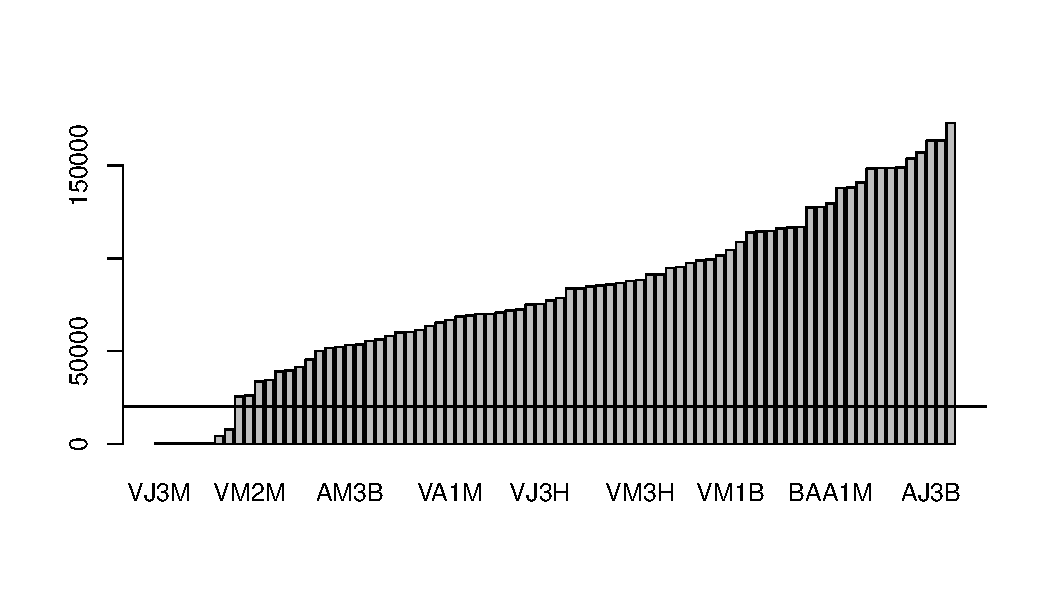
\includegraphics[width=\maxwidth]{figure/unnamed-chunk-12-1} 

}

\caption[Number of sequences by sample]{Number of sequences by sample}\label{fig:unnamed-chunk-12}
\end{figure}


\end{knitrout}

  \subsection{Filter OTUs by number of samples}

First, we can visualize the number of OTU present in a given number of samples (Figure \ref{fig:nbOtu_sample}).

\begin{knitrout}\small
\definecolor{shadecolor}{rgb}{0.969, 0.969, 0.969}\color{fgcolor}\begin{kframe}
\begin{alltt}
\hlstd{df_nbOtu_sample} \hlkwb{<-} \hlkwd{data.frame}\hlstd{(}\hlstr{"Nb of OTUs"} \hlstd{=} \hlkwd{table}\hlstd{(}\hlkwd{rowSums}\hlstd{(}\hlkwd{as.binaryOtuTable}\hlstd{(}
  \hlstd{data.f1)}\hlopt{@}\hlkwc{otu_table}\hlstd{))[}\hlkwd{table}\hlstd{(}\hlkwd{rowSums}\hlstd{(}\hlkwd{as.binaryOtuTable}\hlstd{(data.f1)}\hlopt{@}\hlkwc{otu_table}\hlstd{))} \hlopt{>} \hlnum{1}\hlstd{],}
  \hlstr{"Nb samples"} \hlstd{=} \hlkwd{as.numeric}\hlstd{(}\hlkwd{names}\hlstd{(}\hlkwd{table}\hlstd{(}\hlkwd{rowSums}\hlstd{(}\hlkwd{as.binaryOtuTable}\hlstd{(data.f1)}\hlopt{@}\hlkwc{otu_table}\hlstd{))}
                            \hlstd{[}\hlkwd{table}\hlstd{(}\hlkwd{rowSums}\hlstd{(}\hlkwd{as.binaryOtuTable}\hlstd{(data.f1)}\hlopt{@}\hlkwc{otu_table}\hlstd{))} \hlopt{>} \hlnum{1}\hlstd{])))}

\hlstd{g} \hlkwb{<-} \hlkwd{ggplot}\hlstd{(df_nbOtu_sample,} \hlkwd{aes}\hlstd{(}\hlkwc{y} \hlstd{= Nb.of.OTUs.Freq,} \hlkwc{x} \hlstd{= Nb.samples))}
\hlstd{g} \hlopt{+} \hlkwd{geom_point}\hlstd{(}\hlkwc{size} \hlstd{=} \hlnum{4}\hlstd{,} \hlkwc{col} \hlstd{=} \hlkwd{rgb}\hlstd{(}\hlnum{0.1}\hlstd{,} \hlnum{0.1}\hlstd{,} \hlnum{0.1}\hlstd{,} \hlnum{0.5}\hlstd{))} \hlopt{+}
  \hlkwd{scale_y_continuous}\hlstd{(}\hlkwc{trans} \hlstd{=} \hlstr{'log10'}\hlstd{)} \hlopt{+}
  \hlkwd{geom_smooth}\hlstd{(}\hlkwc{size} \hlstd{=} \hlnum{2}\hlstd{,} \hlkwc{col} \hlstd{=} \hlkwd{rgb}\hlstd{(}\hlnum{0.1}\hlstd{,} \hlnum{0.1}\hlstd{,} \hlnum{0.1}\hlstd{,} \hlnum{0.5}\hlstd{))}

\hlkwd{summary}\hlstd{(df_nbOtu_sample}\hlopt{$}\hlstd{Nb.samples)}
\end{alltt}
\begin{verbatim}
##    Min. 1st Qu.  Median    Mean 3rd Qu.    Max. 
##    1.00   18.75   36.50   36.50   54.25   72.00
\end{verbatim}
\end{kframe}\begin{figure}

{\centering 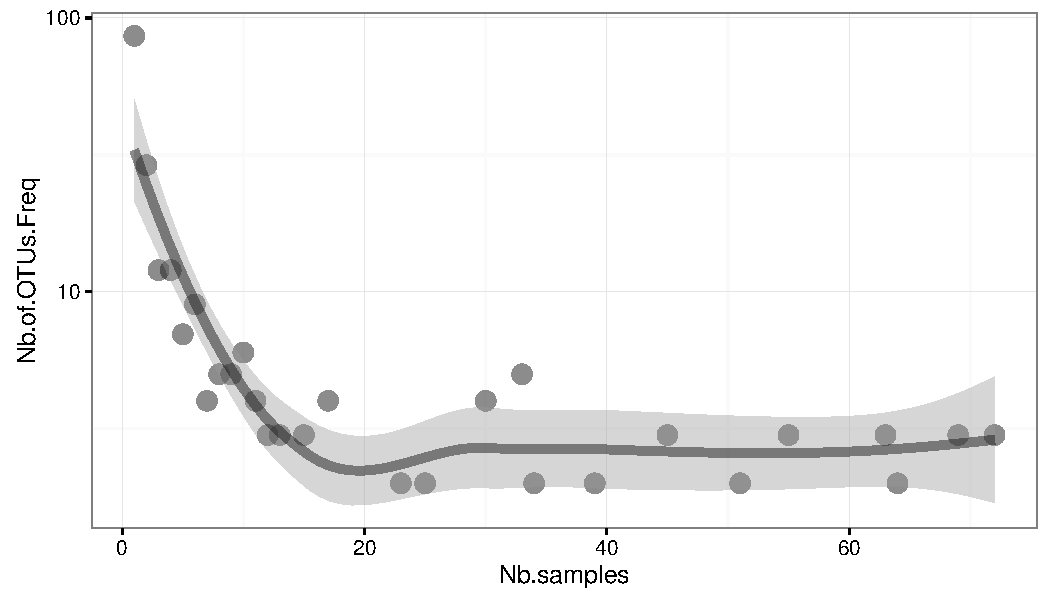
\includegraphics[width=\maxwidth]{figure/nbOtu_sample-1} 

}

\caption[Number of OTU present in a given number of samples]{Number of OTU present in a given number of samples. Vertical bar illustrate the filtering parameter.}\label{fig:nbOtu_sample}
\end{figure}


\end{knitrout}

\begin{knitrout}\small
\definecolor{shadecolor}{rgb}{0.969, 0.969, 0.969}\color{fgcolor}\begin{kframe}
\begin{alltt}
\hlstd{N_otu_sam_min}
\end{alltt}
\begin{verbatim}
## [1] 1
\end{verbatim}
\end{kframe}
\end{knitrout}

\begin{knitrout}\small
\definecolor{shadecolor}{rgb}{0.969, 0.969, 0.969}\color{fgcolor}\begin{kframe}
\begin{alltt}
\hlstd{data.f2} \hlkwb{<-} \hlkwd{prune_taxa}\hlstd{(}\hlkwd{rowSums}\hlstd{(}\hlkwd{as.binaryOtuTable}\hlstd{(data.f1)}\hlopt{@}\hlkwc{otu_table}\hlstd{)} \hlopt{>=}
                        \hlstd{N_otu_sam_min, data.f1)}
\end{alltt}
\end{kframe}
\end{knitrout}

If we discard OTUs present in less than 1 sample, we keep 4359 on the 4359 OTUs (100\%).

 \subsection{Filter OTUs by number of sequences}

 First, we can visualize the number of sequences by OTU (Figure \ref{fig:nbseq_Otu}).

\begin{knitrout}\small
\definecolor{shadecolor}{rgb}{0.969, 0.969, 0.969}\color{fgcolor}\begin{kframe}
\begin{alltt}
\hlstd{df_nbseq_Otu} \hlkwb{<-} \hlkwd{data.frame}\hlstd{(}\hlstr{"Nb of sequences by OTUs"} \hlstd{=} \hlkwd{rowSums}\hlstd{(data.f2}\hlopt{@}\hlkwc{otu_table}\hlstd{))}
\hlstd{g} \hlkwb{<-} \hlkwd{ggplot}\hlstd{(df_nbseq_Otu,} \hlkwd{aes}\hlstd{(}\hlkwc{x} \hlstd{= Nb.of.sequences.by.OTUs))}
\hlstd{g} \hlopt{+} \hlkwd{geom_histogram}\hlstd{(}\hlkwc{size} \hlstd{=} \hlnum{2}\hlstd{,} \hlkwc{col} \hlstd{=} \hlkwd{rgb}\hlstd{(}\hlnum{0.8}\hlstd{,} \hlnum{0.8}\hlstd{,} \hlnum{0.8}\hlstd{,} \hlnum{0.3}\hlstd{))} \hlopt{+}
  \hlkwd{scale_x_continuous}\hlstd{(}\hlkwc{trans} \hlstd{=} \hlstr{'log10'}\hlstd{)} \hlopt{+}
  \hlkwd{geom_vline}\hlstd{(}\hlkwc{xintercept}\hlstd{= N_seq_otu_min)}
\end{alltt}


{\ttfamily\noindent\itshape\color{messagecolor}{\#\# `stat\_bin()` using `bins = 30`. Pick better value with `binwidth`.}}\begin{alltt}
\hlkwd{summary}\hlstd{(df_nbseq_Otu[,} \hlnum{1}\hlstd{])}
\end{alltt}
\begin{verbatim}
##    Min. 1st Qu.  Median    Mean 3rd Qu.    Max. 
##       1       5      22    1922     124  773800
\end{verbatim}
\end{kframe}\begin{figure}

{\centering 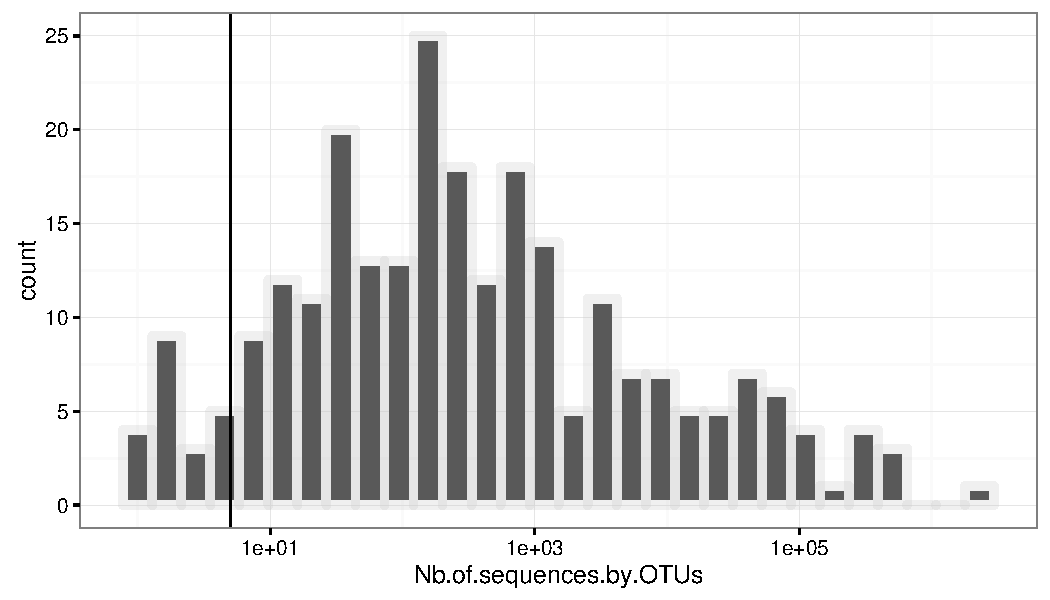
\includegraphics[width=\maxwidth]{figure/nbseq_Otu-1} 

}

\caption[Number of sequences by OTU (log10 transformed)]{Number of sequences by OTU (log10 transformed). Horizontal bar illustrate the filtering parameter.}\label{fig:nbseq_Otu}
\end{figure}


\end{knitrout}

\begin{knitrout}\small
\definecolor{shadecolor}{rgb}{0.969, 0.969, 0.969}\color{fgcolor}\begin{kframe}
\begin{alltt}
\hlstd{N_seq_otu_min}
\end{alltt}
\begin{verbatim}
## [1] 5
\end{verbatim}
\end{kframe}
\end{knitrout}

If we discard OTUs with less than 1 sequences, we keep 3382 on the 4373 OTUs (77.34\%).

\begin{knitrout}\small
\definecolor{shadecolor}{rgb}{0.969, 0.969, 0.969}\color{fgcolor}\begin{kframe}
\begin{alltt}
\hlstd{data.f3} \hlkwb{<-} \hlkwd{prune_taxa}\hlstd{(}\hlkwd{rowSums}\hlstd{(data.f2}\hlopt{@}\hlkwc{otu_table}\hlstd{)} \hlopt{>=} \hlstd{N_seq_otu_min, data.f2)}
\end{alltt}
\end{kframe}
\end{knitrout}

\subsection{Summary of filtration workflow}

The filtered data are made of \ensuremath{8.373567\times 10^{6}} sequences representing 3382 OTUs allocate to 72 samples.




% latex table generated in R 3.3.1 by xtable 1.8-2 package
% Tue Jul 19 18:50:19 2016
\begin{table}[ht]
\centering
\begin{tabular}{rrrr}
  \hline
 & Nb.of.OTUs & Nb.of.samples & Nb.of.sequences \\ 
  \hline
No filter & 4373 &  80 & 8398038.00 \\ 
  Nb of sequences by sample $>$=  20000 & 4359 &  72 & 8375892.00 \\ 
  Nb of sample by OTUs $>$=  1 & 4359 &  72 & 8375892.00 \\ 
  Nb of sequences by OTUs $>$=  5 & 3382 &  72 & 8373567.00 \\ 
   \hline
\end{tabular}
\caption{Number of OTUs, samples and sequences after filtering} 
\end{table}



\section{Simple description of the dataset}

  \subsection{Number of sequences and OTUs by samples}

\begin{knitrout}\small
\definecolor{shadecolor}{rgb}{0.969, 0.969, 0.969}\color{fgcolor}\begin{kframe}
\begin{alltt}
\hlstd{df_nbseq_nbotu} \hlkwb{<-} \hlkwd{data.frame}\hlstd{(}\hlstr{"Nb of sequences by samples"} \hlstd{=} \hlkwd{colSums}\hlstd{(data.f3}\hlopt{@}\hlkwc{otu_table}\hlstd{),}
                             \hlstr{"Nb of OTUs by samples"} \hlstd{=}
                               \hlkwd{colSums}\hlstd{(}\hlkwd{as.binaryOtuTable}\hlstd{(data.f3)}\hlopt{@}\hlkwc{otu_table}\hlstd{))}

\hlstd{g} \hlkwb{<-} \hlkwd{ggplot}\hlstd{(df_nbseq_nbotu,} \hlkwd{aes}\hlstd{(}\hlkwc{x} \hlstd{= Nb.of.OTUs.by.samples,}
                                \hlkwc{y} \hlstd{= Nb.of.sequences.by.samples))}
\hlstd{g} \hlopt{+} \hlkwd{geom_point}\hlstd{(}\hlkwc{size} \hlstd{=} \hlnum{3}\hlstd{,} \hlkwc{col} \hlstd{=} \hlkwd{rgb}\hlstd{(}\hlnum{0.1}\hlstd{,} \hlnum{0.1}\hlstd{,} \hlnum{0.1}\hlstd{,} \hlnum{0.5}\hlstd{))} \hlopt{+}
  \hlkwd{scale_y_continuous}\hlstd{(}\hlkwc{trans} \hlstd{=} \hlstr{'log10'}\hlstd{)} \hlopt{+}
  \hlkwd{geom_smooth}\hlstd{(}\hlkwc{size} \hlstd{=} \hlnum{2}\hlstd{,} \hlkwc{col} \hlstd{=} \hlkwd{rgb}\hlstd{(}\hlnum{0.1}\hlstd{,} \hlnum{0.1}\hlstd{,} \hlnum{0.1}\hlstd{,} \hlnum{0.5}\hlstd{))}
\end{alltt}
\end{kframe}\begin{figure}

{\centering 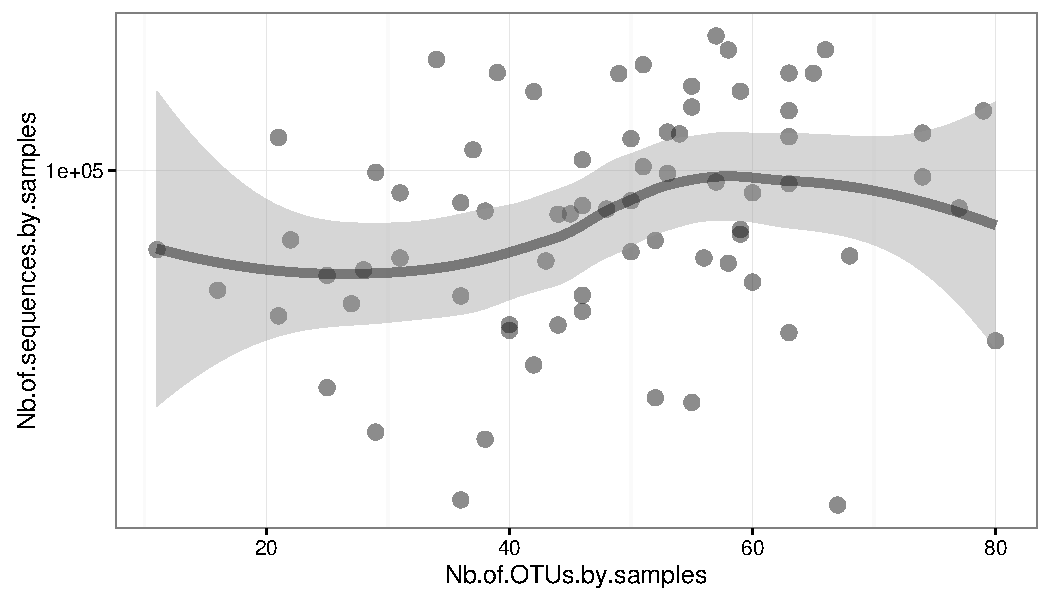
\includegraphics[width=\maxwidth]{figure/unnamed-chunk-19-1} 

}

\caption[Number of OTUs by samples in fonction the number of sequences by samples (log10 axe)]{Number of OTUs by samples in fonction the number of sequences by samples (log10 axe). The tendency is represented by the line obtain from loess (Local Polynomial Regression Fitting).}\label{fig:unnamed-chunk-19}
\end{figure}


\end{knitrout}

\begin{knitrout}\small
\definecolor{shadecolor}{rgb}{0.969, 0.969, 0.969}\color{fgcolor}\begin{kframe}
\begin{alltt}
\hlkwd{ggplot}\hlstd{(}\hlkwd{as.data.frame}\hlstd{(data.f3}\hlopt{@}\hlkwc{refseq}\hlopt{@}\hlkwc{ranges}\hlstd{),} \hlkwd{aes}\hlstd{(}\hlkwc{x} \hlstd{= width))} \hlopt{+} \hlkwd{geom_density}\hlstd{()} \hlopt{+}
  \hlkwd{ylab}\hlstd{(}\hlstr{"Reference sequences length"}\hlstd{)}
\end{alltt}
\end{kframe}\begin{figure}

{\centering 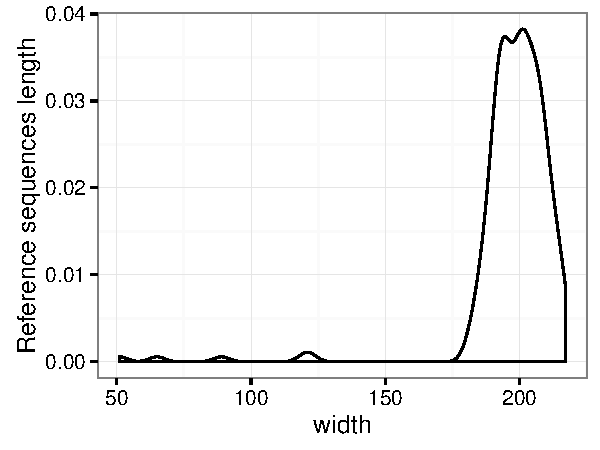
\includegraphics[width=\maxwidth]{figure/unnamed-chunk-20-1} 

}

\caption[Distribution of reference sequences length]{Distribution of reference sequences length.}\label{fig:unnamed-chunk-20}
\end{figure}


\end{knitrout}
 
  \subsection{Number of sequences and samples for each OTUs}
  
\begin{knitrout}\small
\definecolor{shadecolor}{rgb}{0.969, 0.969, 0.969}\color{fgcolor}\begin{kframe}
\begin{alltt}
\hlstd{df_nbseq_nbsam} \hlkwb{<-} \hlkwd{data.frame}\hlstd{(}\hlstr{"Nb of sequences by OTUs"} \hlstd{=} \hlkwd{rowSums}\hlstd{(data.f3}\hlopt{@}\hlkwc{otu_table}\hlstd{)}
                             \hlstd{[}\hlkwd{rowSums}\hlstd{(data.f3}\hlopt{@}\hlkwc{otu_table}\hlstd{)} \hlopt{>} \hlnum{0}\hlstd{],}
                             \hlstr{"Nb of samples by OTUs"} \hlstd{=}
                               \hlkwd{rowSums}\hlstd{(}\hlkwd{as.binaryOtuTable}\hlstd{(data.f3)}\hlopt{@}\hlkwc{otu_table}\hlstd{)}
                             \hlstd{[}\hlkwd{rowSums}\hlstd{(data.f3}\hlopt{@}\hlkwc{otu_table}\hlstd{)} \hlopt{>} \hlnum{0}\hlstd{])}

\hlstd{g} \hlkwb{<-} \hlkwd{ggplot}\hlstd{(df_nbseq_nbsam,} \hlkwd{aes}\hlstd{(}\hlkwc{y} \hlstd{= Nb.of.samples.by.OTUs,}
                                \hlkwc{x} \hlstd{= Nb.of.sequences.by.OTUs))}
\hlstd{g} \hlopt{+} \hlkwd{geom_point}\hlstd{(}\hlkwc{size} \hlstd{=} \hlnum{3}\hlstd{,} \hlkwc{col} \hlstd{=} \hlkwd{rgb}\hlstd{(}\hlnum{0.1}\hlstd{,} \hlnum{0.1}\hlstd{,} \hlnum{0.1}\hlstd{,} \hlnum{0.5}\hlstd{))} \hlopt{+}
  \hlkwd{scale_x_continuous}\hlstd{(}\hlkwc{trans} \hlstd{=} \hlstr{'log10'}\hlstd{)} \hlopt{+}
  \hlkwd{geom_smooth}\hlstd{(}\hlkwc{size} \hlstd{=} \hlnum{2}\hlstd{,} \hlkwc{col} \hlstd{=} \hlkwd{rgb}\hlstd{(}\hlnum{0.1}\hlstd{,} \hlnum{0.1}\hlstd{,} \hlnum{0.1}\hlstd{,} \hlnum{0.5}\hlstd{),} \hlkwc{method} \hlstd{=} \hlstr{"gam"}\hlstd{,}
              \hlkwc{formula}  \hlstd{= y} \hlopt{~} \hlkwd{s}\hlstd{(x,} \hlkwc{bs} \hlstd{=} \hlstr{"cs"}\hlstd{))}
\end{alltt}
\end{kframe}\begin{figure}

{\centering 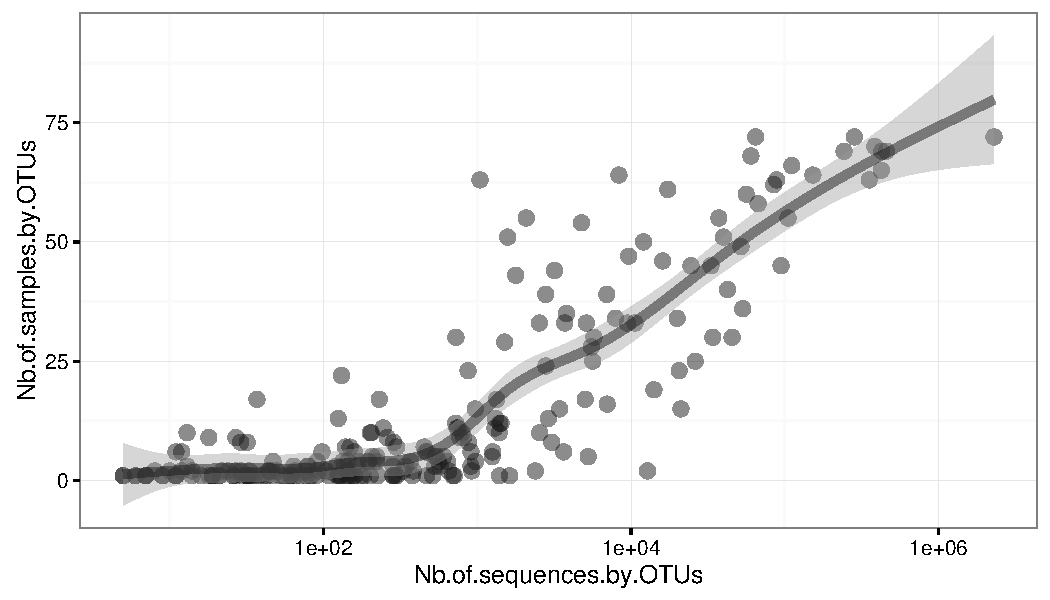
\includegraphics[width=\maxwidth]{figure/unnamed-chunk-21-1} 

}

\caption[Number of sequences by OTUs (log10 axe) in fonction the number of samples where OTUs were found]{Number of sequences by OTUs (log10 axe) in fonction the number of samples where OTUs were found. The tendency is represented by the line obtain from gam (Generalized additive models with integrated smoothness estimation).}\label{fig:unnamed-chunk-21}
\end{figure}


\end{knitrout}

  \subsection{Distribution of sequences in the taxonomy}
\begin{knitrout}\small
\definecolor{shadecolor}{rgb}{0.969, 0.969, 0.969}\color{fgcolor}\begin{kframe}
\begin{alltt}
\hlstd{df3} \hlkwb{<-} \hlkwd{data.frame}\hlstd{(}\hlkwd{as.data.frame}\hlstd{(data.f3}\hlopt{@}\hlkwc{tax_table}\hlstd{),} \hlkwc{nb.seq} \hlstd{=} \hlkwd{rowSums}\hlstd{(data.f3}\hlopt{@}\hlkwc{otu_table}\hlstd{))}
\hlstd{tm} \hlkwb{<-} \hlkwd{treemap}\hlstd{(df3,} \hlkwc{index} \hlstd{=} \hlkwd{c}\hlstd{(}\hlstr{"Order"}\hlstd{,} \hlstr{"Species"}\hlstd{),} \hlkwc{vSize} \hlstd{=} \hlstr{"nb.seq"}\hlstd{,} \hlkwc{vColor} \hlstd{=} \hlstr{"Class"}\hlstd{,}
        \hlkwc{type} \hlstd{=} \hlstr{"categorical"}\hlstd{,} \hlkwc{palette} \hlstd{=} \hlstr{"Paired"}\hlstd{)}
\hlcom{# For an interactive version in html}
\hlcom{# d3tree(tm) }
\end{alltt}
\end{kframe}\begin{figure}

{\centering 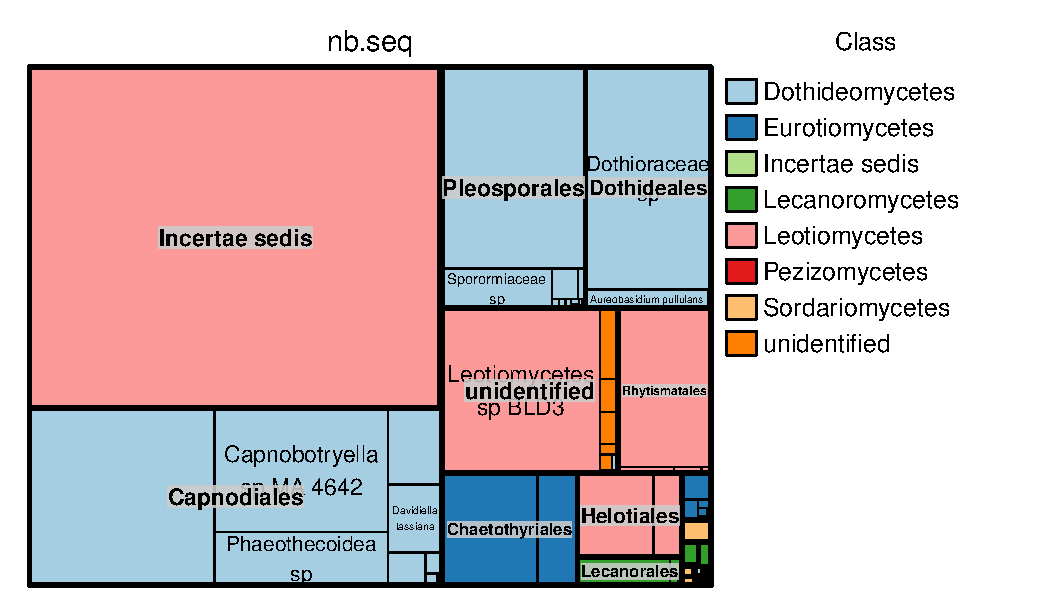
\includegraphics[width=\maxwidth]{figure/unnamed-chunk-22-1} 

}

\caption[Distribution of the number of sequences in the taxonomy]{Distribution of the number of sequences in the taxonomy. Color represent Class, bold lines delimit Order and thick line delimit species.}\label{fig:unnamed-chunk-22}
\end{figure}


\end{knitrout}

\begin{knitrout}\small
\definecolor{shadecolor}{rgb}{0.969, 0.969, 0.969}\color{fgcolor}\begin{kframe}
\begin{alltt}
\hlstd{data.f3_MINSEQ1000} \hlkwb{<-} \hlkwd{subset_taxa}\hlstd{(data.f3,} \hlkwd{rowSums}\hlstd{(data.f3}\hlopt{@}\hlkwc{otu_table}\hlstd{)}\hlopt{>}\hlnum{999}\hlstd{)}
\hlkwd{sankey_phyloseq}\hlstd{(data.f3_MINSEQ1000,} \hlkwc{tax2remove} \hlstd{=}
                  \hlkwd{c}\hlstd{(}\hlstr{"Incertae sedis"}\hlstd{,} \hlstr{"unidentified"}\hlstd{,} \hlstr{"Xylariales"}\hlstd{,} \hlstr{"NA"}\hlstd{),}
                \hlkwc{nbSeq} \hlstd{=} \hlnum{TRUE}\hlstd{,} \hlkwc{taxa} \hlstd{=} \hlkwd{c}\hlstd{(}\hlnum{1}\hlopt{:}\hlnum{6}\hlstd{))}
\end{alltt}
\end{kframe}
\end{knitrout}

\begin{knitrout}\small
\definecolor{shadecolor}{rgb}{0.969, 0.969, 0.969}\color{fgcolor}\begin{kframe}
\begin{alltt}
\hlkwd{sankey_phyloseq}\hlstd{(data.f3,} \hlkwc{tax2remove} \hlstd{=} \hlkwd{c}\hlstd{(}\hlstr{"Incertae sedis"}\hlstd{,} \hlstr{"unidentified"}\hlstd{,} \hlstr{"Xylariales"}\hlstd{),}
                \hlkwc{nbSeq} \hlstd{=} \hlnum{FALSE}\hlstd{,} \hlkwc{taxa} \hlstd{=} \hlkwd{c}\hlstd{(}\hlnum{1}\hlopt{:}\hlnum{5}\hlstd{),} \hlkwc{min.prop.tax} \hlstd{=} \hlnum{0.01}\hlstd{)}
\end{alltt}
\end{kframe}
\end{knitrout}

  \subsection{Focus on the 30 more abundant OTUs (number of sequences)}

\begin{knitrout}\small
\definecolor{shadecolor}{rgb}{0.969, 0.969, 0.969}\color{fgcolor}\begin{kframe}
\begin{alltt}
\hlstd{the30mostfrequents} \hlkwb{<-} \hlkwd{sort}\hlstd{(}\hlkwc{decreasing} \hlstd{= T,} \hlkwd{rowSums}\hlstd{(data.f3}\hlopt{@}\hlkwc{otu_table}\hlstd{))[}\hlnum{1}\hlopt{:}\hlnum{30}\hlstd{]}
\hlkwd{barplot}\hlstd{(the30mostfrequents,} \hlkwc{horiz} \hlstd{= T,} \hlkwc{cex.names} \hlstd{=} \hlnum{0.4}\hlstd{,} \hlkwc{las} \hlstd{=} \hlnum{2}\hlstd{)}
\end{alltt}
\end{kframe}\begin{figure}

{\centering 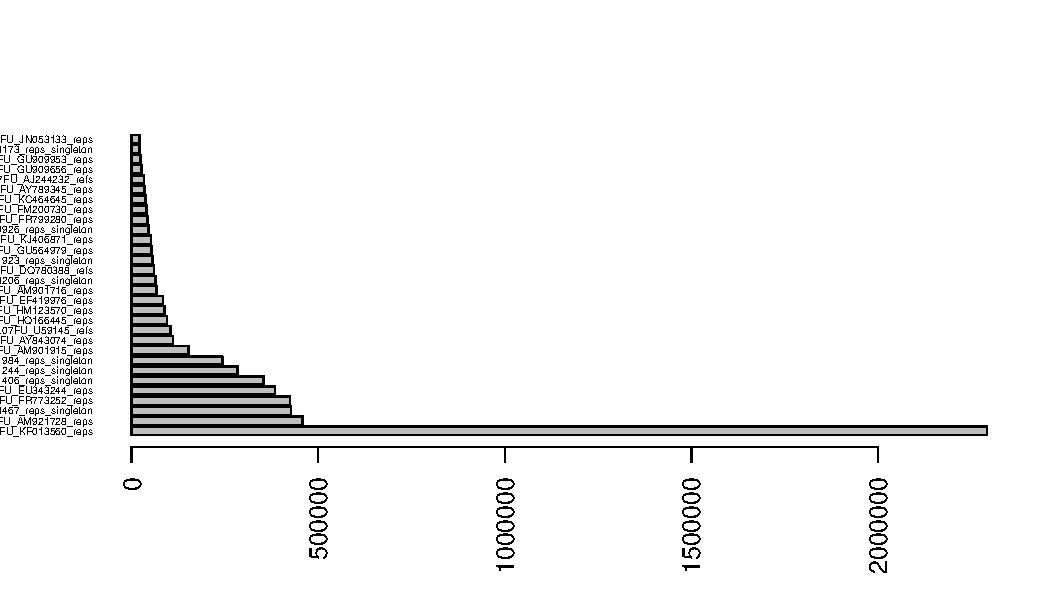
\includegraphics[width=\maxwidth]{figure/unnamed-chunk-25-1} 

}

\caption[Number of sequences of the 30 more abundant OTUs (number of sequences)]{Number of sequences of the 30 more abundant OTUs (number of sequences).}\label{fig:unnamed-chunk-25}
\end{figure}


\end{knitrout}



\begin{landscape}
\begin{kframe}
\begin{alltt}
\hlkwd{print}\hlstd{(}\hlkwd{xtable}\hlstd{(df_the30mostfrequents[,} \hlkwd{c}\hlstd{(}\hlnum{1}\hlopt{:}\hlnum{8}\hlstd{,} \hlnum{12}\hlstd{)],} \hlkwc{auto} \hlstd{= T,}
             \hlkwc{caption} \hlstd{=} \hlstr{"Taxonomie of the 30 more
             frequent OTUs (number of sequences)"}\hlstd{),}
      \hlkwc{size} \hlstd{=} \hlstr{"\textbackslash{}\textbackslash{}tiny"}\hlstd{,} \hlkwc{include.rownames} \hlstd{=} \hlnum{FALSE}\hlstd{)}
\end{alltt}
\end{kframe}% latex table generated in R 3.3.1 by xtable 1.8-2 package
% Tue Jul 19 18:50:21 2016
\begin{table}[ht]
\centering
\begingroup\tiny
\begin{tabular}{llllllllr}
  \hline
Phylum & Class & Order & Family & Genus & Species & Trophic\_Mode & Guild & Nb.sequences \\ 
  \hline
Ascomycota & Leotiomycetes & Incertae sedis & Incertae sedis & Cyclaneusma & Cyclaneusma minus & - & - & 773785 \\ 
  Ascomycota & Leotiomycetes & Incertae sedis & Incertae sedis & Cyclaneusma & Cyclaneusma minus & - & - & 602702 \\ 
  Ascomycota & Leotiomycetes & Incertae sedis & Incertae sedis & Cyclaneusma & Cyclaneusma minus & - & - & 496770 \\ 
  Ascomycota & Dothideomycetes & Pleosporales &  &  &  & - & - & 411106 \\ 
  Ascomycota & Dothideomycetes & Dothideales & Dothioraceae & unidentified & Dothioraceae sp & - & - & 384457 \\ 
  Ascomycota & Dothideomycetes & Capnodiales & Incertae sedis & Capnobotryella & Capnobotryella sp MA 4642 & Saprotroph & Undefined Saprotroph & 334181 \\ 
  Ascomycota & Dothideomycetes & Pleosporales &  &  &  & - & - & 253023 \\ 
  Ascomycota & Dothideomycetes & Capnodiales &  &  &  & - & - & 217662 \\ 
  Ascomycota & Dothideomycetes & Pleosporales &  &  &  & - & - & 175339 \\ 
  Ascomycota & Leotiomycetes & unidentified & unidentified & unidentified & Leotiomycetes sp BLD3 & - & - & 165973 \\ 
  Ascomycota & Leotiomycetes & unidentified & unidentified & unidentified & Leotiomycetes sp BLD3 & - & - & 162700 \\ 
  Ascomycota & Dothideomycetes & Pleosporales &  &  &  & - & - & 156134 \\ 
  Ascomycota & Dothideomycetes & Capnodiales & Mycosphaerellaceae & Phaeothecoidea & Phaeothecoidea sp & Saprotroph & Undefined Saprotroph & 146545 \\ 
   &  &  &  &  &  & - & - & 134866 \\ 
   &  &  &  &  &  & - & - & 112125 \\ 
  Ascomycota & Leotiomycetes & Rhytismatales & Rhytismataceae & Lophodermium & Lophodermium conigenum & Pathotroph & Plant Pathogen & 100144 \\ 
   &  &  &  &  &  & - & - & 85558 \\ 
  Ascomycota & Eurotiomycetes & Chaetothyriales & Herpotrichiellaceae & Phaeomoniella & Phaeomoniella sp & Saprotroph & Undefined Saprotroph & 84162 \\ 
  Ascomycota & Dothideomycetes & Capnodiales &  &  &  & - & - & 83661 \\ 
   &  &  &  &  &  & - & - & 79960 \\ 
   &  &  &  &  &  & - & - & 78582 \\ 
  Ascomycota & Leotiomycetes & Incertae sedis & Incertae sedis & Cyclaneusma & Cyclaneusma minus & - & - & 77326 \\ 
  Ascomycota & Leotiomycetes & unidentified & unidentified & unidentified & Leotiomycetes sp BLD3 & - & - & 76859 \\ 
  Ascomycota & Leotiomycetes & Incertae sedis & Incertae sedis & Cyclaneusma & Cyclaneusma minus & - & - & 73000 \\ 
  unidentified & unidentified & unidentified & unidentified & unidentified & fungal sp TRN287 & - & - & 69266 \\ 
  Ascomycota & Eurotiomycetes & Chaetothyriales & Herpotrichiellaceae & Phaeomoniella & Phaeomoniella sp & Saprotroph & Undefined Saprotroph & 61167 \\ 
  Ascomycota & Dothideomycetes & Capnodiales &  &  &  & - & - & 59701 \\ 
   &  &  &  &  &  & - & - & 59694 \\ 
  Ascomycota & Leotiomycetes & Rhytismatales & Rhytismataceae & Lophodermium &  & Pathotroph & Plant Pathogen & 59517 \\ 
   \hline
\end{tabular}
\endgroup
\caption{Taxonomie of the 30 more
             frequent OTUs (number of sequences)} 
\end{table}

\end{landscape}

\begin{knitrout}\small
\definecolor{shadecolor}{rgb}{0.969, 0.969, 0.969}\color{fgcolor}\begin{kframe}
\begin{alltt}
\hlkwd{treemap}\hlstd{(df_the30mostfrequents,} \hlkwc{index} \hlstd{=} \hlkwd{c}\hlstd{(}\hlstr{"Class"}\hlstd{,} \hlstr{"Species"}\hlstd{),} \hlkwc{vSize} \hlstd{=} \hlstr{"Nb.sequences"}\hlstd{,}
        \hlkwc{vColor} \hlstd{=} \hlstr{"Order"}\hlstd{,} \hlkwc{type} \hlstd{=} \hlstr{"categorical"}\hlstd{,} \hlkwc{palette} \hlstd{=} \hlstr{"Paired"}\hlstd{)}
\end{alltt}
\end{kframe}\begin{figure}

{\centering 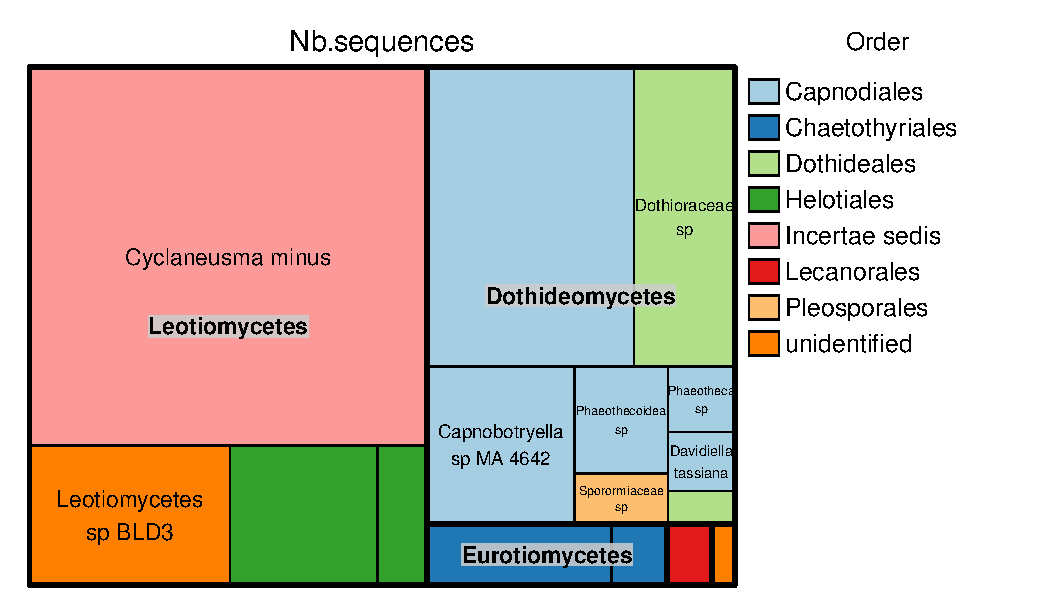
\includegraphics[width=\maxwidth]{figure/unnamed-chunk-28-1} 

}

\caption[Number of sequences of the 30 most abundant OTUs (number of sequences)]{Number of sequences of the 30 most abundant OTUs (number of sequences). Colors indicate Order, bold lines delimit Class and thick lines delimit species.}\label{fig:unnamed-chunk-28}
\end{figure}


\end{knitrout}

  \subsection{Focus on the 30 more frequent OTUs (number of samples)}

\begin{knitrout}\small
\definecolor{shadecolor}{rgb}{0.969, 0.969, 0.969}\color{fgcolor}\begin{kframe}
\begin{alltt}
\hlstd{the30mostfrequents_samp} \hlkwb{<-} \hlkwd{sort}\hlstd{(}\hlkwc{decreasing} \hlstd{= T,}
                                \hlkwd{rowSums}\hlstd{(}\hlkwd{as.binaryOtuTable}\hlstd{(data.f3)}\hlopt{@}\hlkwc{otu_table}\hlstd{))[}\hlnum{1}\hlopt{:}\hlnum{30}\hlstd{]}
\hlkwd{barplot}\hlstd{(the30mostfrequents_samp,} \hlkwc{horiz} \hlstd{= T,} \hlkwc{cex.names} \hlstd{=} \hlnum{0.4}\hlstd{,} \hlkwc{las} \hlstd{=} \hlnum{2}\hlstd{)}
\end{alltt}
\end{kframe}\begin{figure}

{\centering 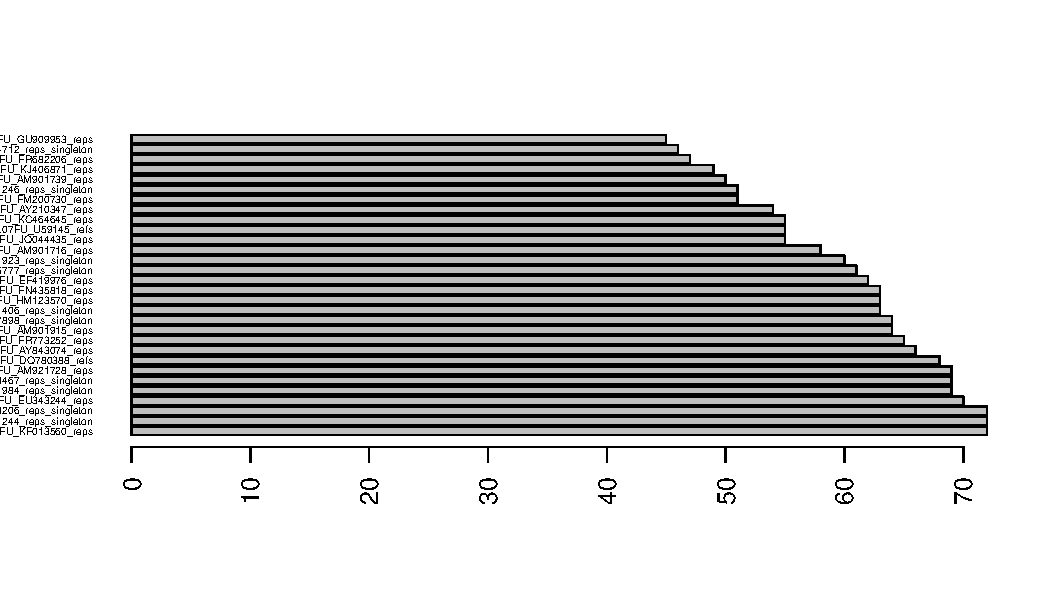
\includegraphics[width=\maxwidth]{figure/unnamed-chunk-29-1} 

}

\caption[Number of samples of the 30 more frequent OTUs (number of samples)]{Number of samples of the 30 more frequent OTUs (number of samples).}\label{fig:unnamed-chunk-29}
\end{figure}


\end{knitrout}




\begin{landscape}
\begin{kframe}
\begin{alltt}
\hlkwd{print}\hlstd{(}\hlkwd{xtable}\hlstd{(df_the30mostfrequents_samp[,} \hlkwd{c}\hlstd{(}\hlnum{1}\hlopt{:}\hlnum{8}\hlstd{,} \hlnum{12}\hlstd{)],} \hlkwc{auto} \hlstd{= T,}
      \hlkwc{caption} \hlstd{=} \hlstr{"Taxonomie of the 30 more frequent OTUs (number of samples)"}\hlstd{),}
      \hlkwc{size} \hlstd{=} \hlstr{"\textbackslash{}\textbackslash{}tiny"}\hlstd{,} \hlkwc{include.rownames} \hlstd{=} \hlnum{FALSE}\hlstd{)}
\end{alltt}
\end{kframe}% latex table generated in R 3.3.1 by xtable 1.8-2 package
% Tue Jul 19 18:50:22 2016
\begin{table}[ht]
\centering
\begingroup\tiny
\begin{tabular}{llllllllr}
  \hline
Phylum & Class & Order & Family & Genus & Species & Trophic\_Mode & Guild & Nb.samples \\ 
  \hline
Ascomycota & Leotiomycetes & Incertae sedis & Incertae sedis & Cyclaneusma & Cyclaneusma minus & - & - & 72 \\ 
  Ascomycota & Leotiomycetes & Incertae sedis & Incertae sedis & Cyclaneusma & Cyclaneusma minus & - & - & 72 \\ 
  Ascomycota & Leotiomycetes & Incertae sedis & Incertae sedis & Cyclaneusma & Cyclaneusma minus & - & - & 72 \\ 
  Ascomycota & Leotiomycetes & Incertae sedis & Incertae sedis & Cyclaneusma & Cyclaneusma minus & - & - & 72 \\ 
  Ascomycota & Leotiomycetes & Incertae sedis & Incertae sedis & Cyclaneusma & Cyclaneusma minus & - & - & 72 \\ 
  Ascomycota & Leotiomycetes & Incertae sedis & Incertae sedis & Cyclaneusma & Cyclaneusma minus & - & - & 72 \\ 
  Ascomycota & Leotiomycetes & Incertae sedis & Incertae sedis & Cyclaneusma & Cyclaneusma minus & - & - & 72 \\ 
  Ascomycota & Leotiomycetes & Incertae sedis & Incertae sedis & Cyclaneusma & Cyclaneusma minus & - & - & 72 \\ 
  Ascomycota & Leotiomycetes & Incertae sedis & Incertae sedis & Cyclaneusma & Cyclaneusma minus & - & - & 72 \\ 
  Ascomycota & Leotiomycetes & Incertae sedis & Incertae sedis & Cyclaneusma & Cyclaneusma minus & - & - & 72 \\ 
  Ascomycota & Leotiomycetes & Incertae sedis & Incertae sedis & Cyclaneusma & Cyclaneusma minus & - & - & 72 \\ 
  Ascomycota & Leotiomycetes & Incertae sedis & Incertae sedis & Cyclaneusma & Cyclaneusma minus & - & - & 72 \\ 
  Ascomycota & Leotiomycetes & Incertae sedis & Incertae sedis & Cyclaneusma & Cyclaneusma minus & - & - & 71 \\ 
  Ascomycota & Leotiomycetes & Incertae sedis & Incertae sedis & Cyclaneusma & Cyclaneusma minus & - & - & 71 \\ 
  Ascomycota & Leotiomycetes & Incertae sedis & Incertae sedis & Cyclaneusma & Cyclaneusma minus & - & - & 71 \\ 
  Ascomycota & Leotiomycetes & Incertae sedis & Incertae sedis & Cyclaneusma & Cyclaneusma minus & - & - & 71 \\ 
  Ascomycota & Leotiomycetes & Incertae sedis & Incertae sedis & Cyclaneusma & Cyclaneusma minus & - & - & 71 \\ 
  Ascomycota & Leotiomycetes & Incertae sedis & Incertae sedis & Cyclaneusma & Cyclaneusma minus & - & - & 71 \\ 
   \hline
\end{tabular}
\endgroup
\caption{Taxonomie of the 30 more frequent OTUs (number of samples)} 
\end{table}

\end{landscape}


\section{Number of sequences and OTUs in function of putative ecology (using FUNGuild software; Nguyen et al, 2015)}

\begin{knitrout}\small
\definecolor{shadecolor}{rgb}{0.969, 0.969, 0.969}\color{fgcolor}\begin{kframe}
\begin{alltt}
\hlstd{tabPutativeEcology} \hlkwb{<-} \hlkwd{apply}\hlstd{(data.f3}\hlopt{@}\hlkwc{tax_table}\hlstd{,} \hlnum{2}\hlstd{,} \hlkwa{function}\hlstd{(}\hlkwc{x}\hlstd{)} \hlkwd{table}\hlstd{(x))}
\hlstd{tabPutativeEcology_percent} \hlkwb{<-} \hlkwd{apply}\hlstd{(data.f3}\hlopt{@}\hlkwc{tax_table}\hlstd{,} \hlnum{2}\hlstd{,} \hlkwa{function}\hlstd{(}\hlkwc{x}\hlstd{)}
  \hlkwd{round}\hlstd{(}\hlkwd{table}\hlstd{(x)}\hlopt{/}\hlkwd{dim}\hlstd{(data.f3}\hlopt{@}\hlkwc{tax_table}\hlstd{)[}\hlnum{1}\hlstd{]}\hlopt{*}\hlnum{100}\hlstd{,} \hlnum{3}\hlstd{))}
\hlkwd{sum}\hlstd{(data.f3}\hlopt{@}\hlkwc{otu_table}\hlstd{[data.f3}\hlopt{@}\hlkwc{tax_table}\hlstd{[,}\hlstr{"Trophic_Mode"}\hlstd{]}\hlopt{==}\hlstr{"-"}\hlstd{])} \hlopt{/}
  \hlkwd{sum}\hlstd{(data.f3}\hlopt{@}\hlkwc{otu_table}\hlstd{)}\hlopt{*}\hlnum{100}
\end{alltt}
\begin{verbatim}
## [1] 81.36235
\end{verbatim}
\begin{alltt}
\hlstd{tmdata} \hlkwb{<-} \hlkwd{as.data.frame}\hlstd{(data.f3}\hlopt{@}\hlkwc{tax_table}\hlstd{[data.f3}\hlopt{@}\hlkwc{tax_table}\hlstd{[,}\hlstr{"Trophic_Mode"}\hlstd{]}\hlopt{!=}\hlstr{"-"}\hlstd{])}
\hlstd{tmdata}\hlopt{$}\hlstd{Nb.sequences} \hlkwb{<-} \hlkwd{rowSums}\hlstd{(data.f3}\hlopt{@}\hlkwc{otu_table}\hlstd{[data.f3}\hlopt{@}\hlkwc{tax_table}\hlstd{[,}\hlstr{"Trophic_Mode"}\hlstd{]}\hlopt{!=}\hlstr{"-"}\hlstd{])}
\hlstd{tmdata}\hlopt{$}\hlstd{Nb.OTU} \hlkwb{<-} \hlkwd{rep}\hlstd{(}\hlnum{1}\hlstd{,} \hlkwd{length}\hlstd{(tmdata}\hlopt{$}\hlstd{Nb.sequences))}
\end{alltt}
\end{kframe}
\end{knitrout}

\begin{knitrout}\small
\definecolor{shadecolor}{rgb}{0.969, 0.969, 0.969}\color{fgcolor}\begin{kframe}
\begin{alltt}
\hlkwd{ggplot}\hlstd{(tmdata)} \hlopt{+} \hlkwd{geom_bar}\hlstd{(}\hlkwd{aes}\hlstd{(}\hlkwc{x}\hlstd{= Trophic_Mode,} \hlkwc{fill}\hlstd{=Guild),} \hlkwc{position} \hlstd{=} \hlstr{"dodge"}\hlstd{)} \hlopt{+}
  \hlkwd{scale_fill_discrete}\hlstd{(}\hlstr{"Paired"}\hlstd{)}\hlopt{+} \hlkwd{theme_grey}\hlstd{()}
\end{alltt}
\end{kframe}\begin{figure}

{\centering 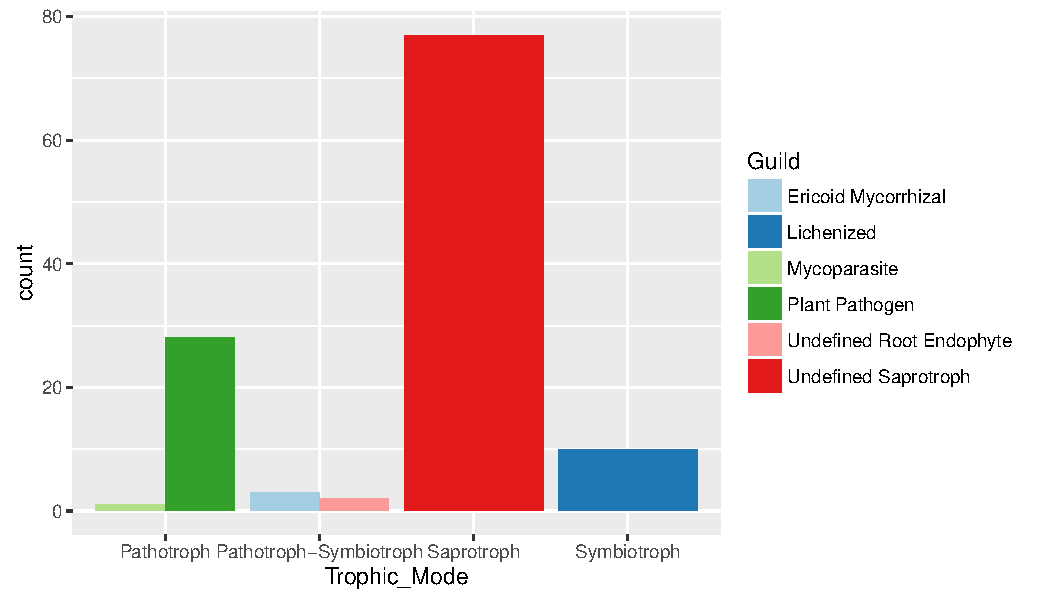
\includegraphics[width=\maxwidth]{figure/unnamed-chunk-33-1} 

}

\caption[Distribution of OTUs into functional Guild]{Distribution of OTUs into functional Guild.}\label{fig:unnamed-chunk-33}
\end{figure}


\end{knitrout}

\begin{knitrout}\small
\definecolor{shadecolor}{rgb}{0.969, 0.969, 0.969}\color{fgcolor}\begin{kframe}
\begin{alltt}
\hlkwd{ggplot}\hlstd{(tmdata,} \hlkwc{stat}\hlstd{=}\hlstr{"identity"}\hlstd{)} \hlopt{+}
  \hlkwd{geom_bar}\hlstd{(}\hlkwd{aes}\hlstd{(}\hlkwc{x}\hlstd{= Trophic_Mode,} \hlkwc{weight} \hlstd{= Nb.sequences,}  \hlkwc{fill}\hlstd{=Guild),} \hlkwc{position} \hlstd{=} \hlstr{"dodge"}\hlstd{)} \hlopt{+}
  \hlkwd{scale_fill_discrete}\hlstd{(}\hlstr{"Paired"}\hlstd{)} \hlopt{+} \hlkwd{scale_y_log10}\hlstd{()} \hlopt{+} \hlkwd{theme_grey}\hlstd{()}
\end{alltt}
\end{kframe}\begin{figure}

{\centering 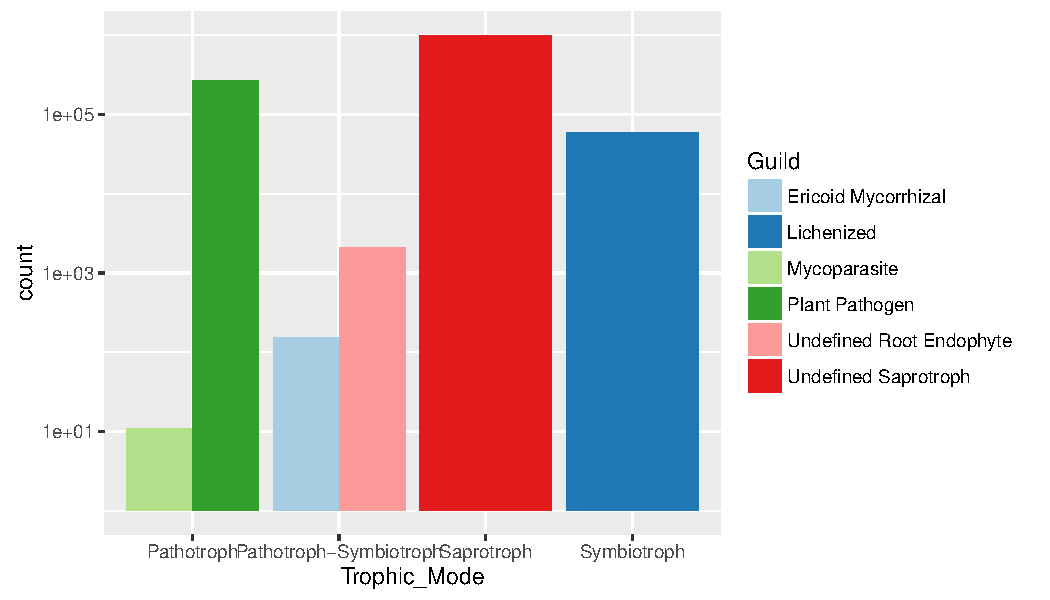
\includegraphics[width=\maxwidth]{figure/unnamed-chunk-34-1} 

}

\caption[Distribution of sequences (log10 transformed) into functional Guild]{Distribution of sequences (log10 transformed) into functional Guild.}\label{fig:unnamed-chunk-34}
\end{figure}


\end{knitrout}

\section{Distribution of fungal endophytic alpha-biodiversity}
  \subsection{Local diversity = Diversity by sites}
  
\begin{knitrout}\small
\definecolor{shadecolor}{rgb}{0.969, 0.969, 0.969}\color{fgcolor}\begin{kframe}
\begin{alltt}
\hlkwd{accu_plot}\hlstd{(data.f3,} \hlstr{"Sites"}\hlstd{,} \hlkwc{nbSeq} \hlstd{=} \hlnum{FALSE}\hlstd{)}
\end{alltt}
\end{kframe}\begin{figure}

{\centering 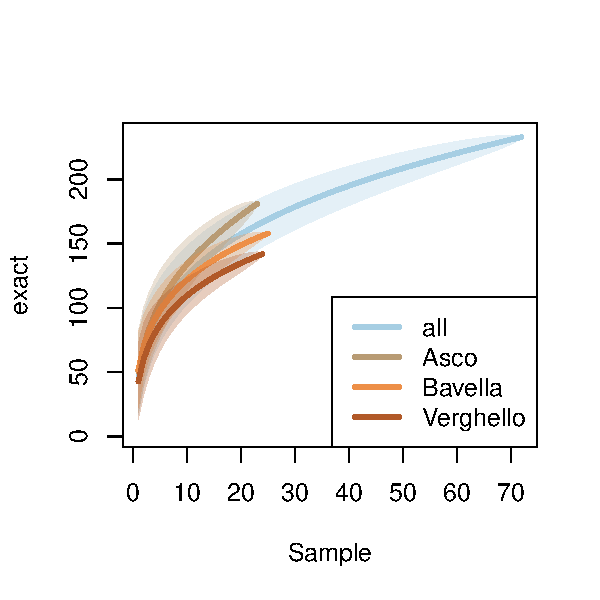
\includegraphics[width=\maxwidth]{figure/unnamed-chunk-35-1} 

}

\caption[Rarefaction curves for each sites]{Rarefaction curves for each sites. Notes that if singletons were removed, these curves are biaised.}\label{fig:unnamed-chunk-35}
\end{figure}


\end{knitrout}

\begin{knitrout}\small
\definecolor{shadecolor}{rgb}{0.969, 0.969, 0.969}\color{fgcolor}\begin{kframe}
\begin{alltt}
\hlkwd{accu_plot}\hlstd{(data.f3,} \hlstr{"Sites"}\hlstd{,} \hlkwc{step} \hlstd{=} \hlnum{5000}\hlstd{)}
\end{alltt}
\end{kframe}\begin{figure}

{\centering 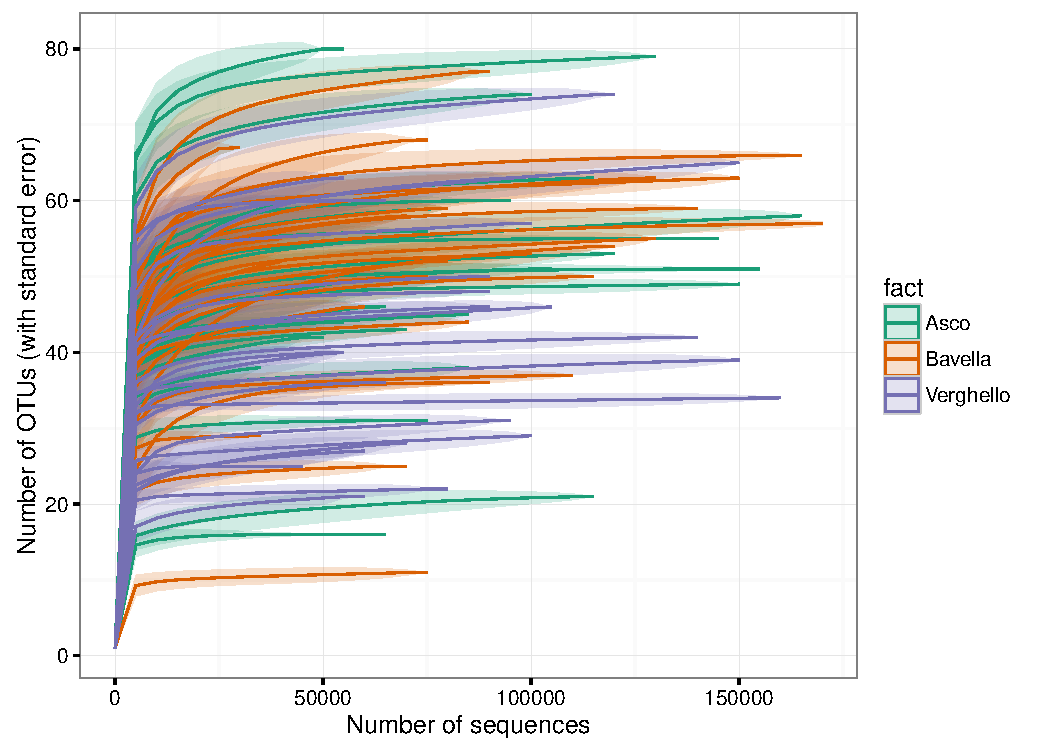
\includegraphics[width=\maxwidth]{figure/unnamed-chunk-36-1} 

}

\caption[Rarefaction curves for each samples using sequences number on x-axes]{Rarefaction curves for each samples using sequences number on x-axes. Notes that if singletons were removed, these curves are biaised.}\label{fig:unnamed-chunk-36}
\end{figure}


\end{knitrout}

\begin{knitrout}\small
\definecolor{shadecolor}{rgb}{0.969, 0.969, 0.969}\color{fgcolor}\begin{kframe}
\begin{alltt}
\hlstd{measures_index} \hlkwb{<-} \hlkwd{c}\hlstd{(}\hlstr{"Observed"}\hlstd{,} \hlstr{"Chao1"}\hlstd{,} \hlstr{"Shannon"}\hlstd{,} \hlstr{"Simpson"}\hlstd{)}
\hlstd{p} \hlkwb{<-} \hlkwd{plot_richness}\hlstd{(data.f3,} \hlkwc{x} \hlstd{=} \hlstr{"Sites"}\hlstd{,} \hlkwc{color} \hlstd{=} \hlstr{"Sites"}\hlstd{,} \hlkwc{measures} \hlstd{= measures_index)}
\hlstd{p} \hlopt{+} \hlkwd{geom_boxplot}\hlstd{(}\hlkwc{data} \hlstd{= p}\hlopt{$}\hlstd{data,} \hlkwc{alpha} \hlstd{=} \hlnum{0.5}\hlstd{)}
\end{alltt}
\end{kframe}\begin{figure}

{\centering 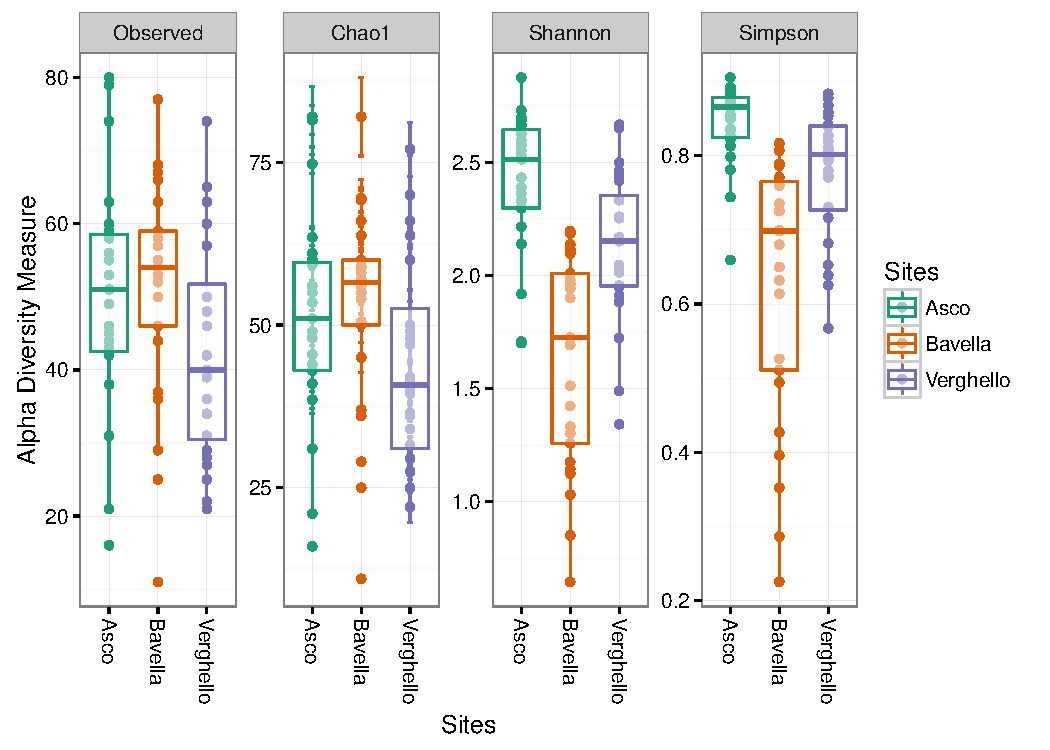
\includegraphics[width=\maxwidth]{figure/unnamed-chunk-37-1} 

}

\caption[Diversity of each sites]{Diversity of each sites}\label{fig:unnamed-chunk-37}
\end{figure}


\end{knitrout}

  \subsection{Diversity by age of tree}
  
\begin{knitrout}\small
\definecolor{shadecolor}{rgb}{0.969, 0.969, 0.969}\color{fgcolor}\begin{kframe}
\begin{alltt}
\hlkwd{accu_plot}\hlstd{(data.f3,} \hlstr{"Age"}\hlstd{,} \hlkwc{nbSeq} \hlstd{=} \hlnum{FALSE}\hlstd{)}
\end{alltt}
\end{kframe}\begin{figure}

{\centering 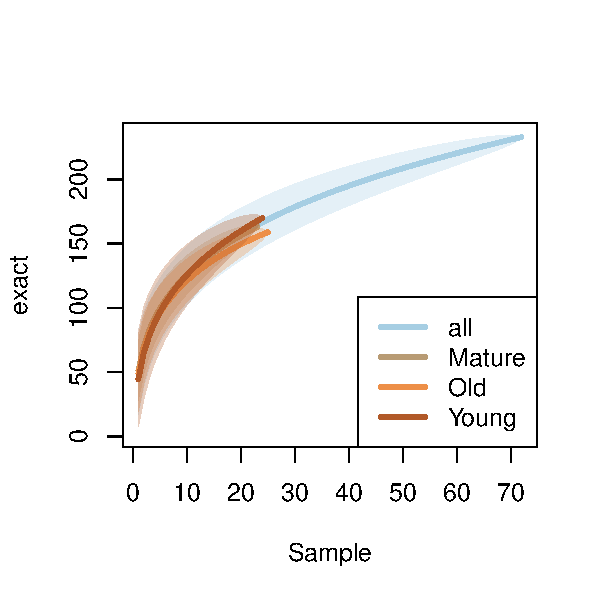
\includegraphics[width=\maxwidth]{figure/unnamed-chunk-38-1} 

}

\caption[Rarefaction curves for each tree age modalities]{Rarefaction curves for each tree age modalities. Notes that if singletons were removed, these curves are biaised.}\label{fig:unnamed-chunk-38}
\end{figure}


\end{knitrout}
  
\begin{knitrout}\small
\definecolor{shadecolor}{rgb}{0.969, 0.969, 0.969}\color{fgcolor}\begin{kframe}
\begin{alltt}
\hlstd{measures_index} \hlkwb{<-} \hlkwd{c}\hlstd{(}\hlstr{"Observed"}\hlstd{,} \hlstr{"Chao1"}\hlstd{,} \hlstr{"Shannon"}\hlstd{,} \hlstr{"Simpson"}\hlstd{)}
\hlstd{p} \hlkwb{<-} \hlkwd{plot_richness}\hlstd{(data.f3,} \hlkwc{x} \hlstd{=} \hlstr{"Age"}\hlstd{,} \hlkwc{color} \hlstd{=} \hlstr{"Sites"}\hlstd{,} \hlkwc{measures} \hlstd{= measures_index)}
\hlstd{p} \hlopt{+} \hlkwd{geom_boxplot}\hlstd{(}\hlkwc{data} \hlstd{= p}\hlopt{$}\hlstd{data,} \hlkwd{aes}\hlstd{(}\hlkwc{x} \hlstd{= p}\hlopt{$}\hlstd{data}\hlopt{$}\hlstd{Age,} \hlkwc{y} \hlstd{= value,} \hlkwc{color} \hlstd{=} \hlkwa{NULL}\hlstd{),}
                 \hlkwc{alpha} \hlstd{=} \hlnum{0.5}\hlstd{)}
\end{alltt}
\end{kframe}\begin{figure}

{\centering 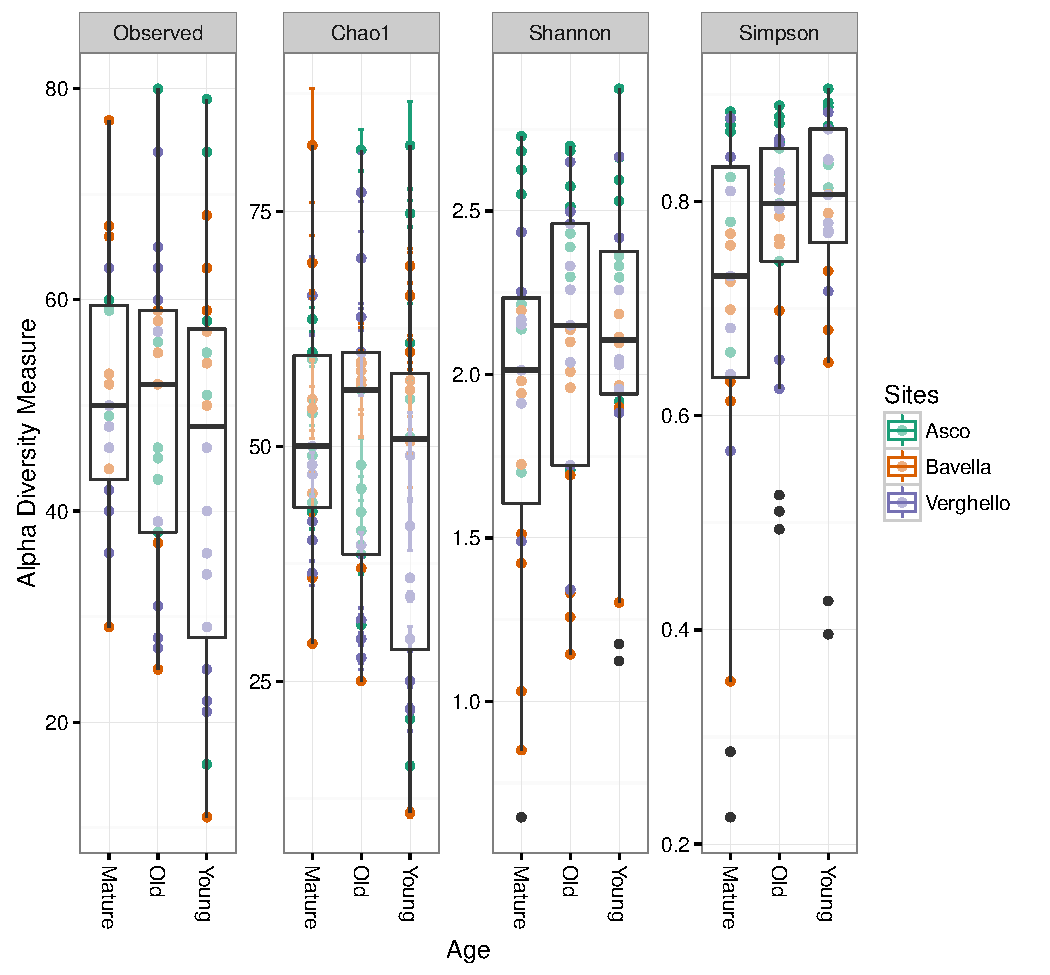
\includegraphics[width=\maxwidth]{figure/unnamed-chunk-39-1} 

}

\caption[Diversity in function of tree age]{Diversity in function of tree age. Color represent sites.}\label{fig:unnamed-chunk-39}
\end{figure}


\end{knitrout}

  \subsection{Diversity by elevation of the sample}

\begin{knitrout}\small
\definecolor{shadecolor}{rgb}{0.969, 0.969, 0.969}\color{fgcolor}\begin{kframe}
\begin{alltt}
\hlkwd{accu_plot}\hlstd{(data.f3,} \hlstr{"Elevation"}\hlstd{,} \hlkwc{nbSeq} \hlstd{=} \hlnum{FALSE}\hlstd{)}
\end{alltt}
\end{kframe}\begin{figure}

{\centering 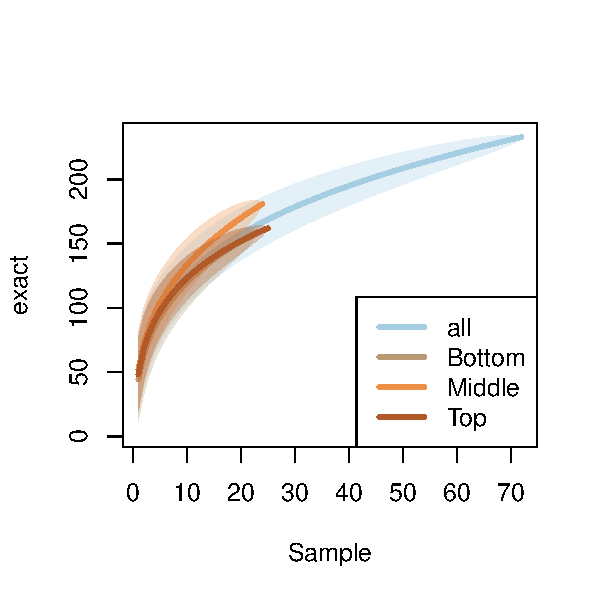
\includegraphics[width=\maxwidth]{figure/unnamed-chunk-40-1} 

}

\caption[Rarefaction curves for each elevation]{Rarefaction curves for each elevation. Notes that if singletons were removed, these curves are biaised.}\label{fig:unnamed-chunk-40}
\end{figure}


\end{knitrout}

\begin{knitrout}\small
\definecolor{shadecolor}{rgb}{0.969, 0.969, 0.969}\color{fgcolor}\begin{kframe}
\begin{alltt}
\hlstd{measures_index} \hlkwb{<-} \hlkwd{c}\hlstd{(}\hlstr{"Observed"}\hlstd{,} \hlstr{"Chao1"}\hlstd{,} \hlstr{"Shannon"}\hlstd{,} \hlstr{"Simpson"}\hlstd{)}
\hlstd{p} \hlkwb{<-} \hlkwd{plot_richness}\hlstd{(data.f3,} \hlkwc{x} \hlstd{=} \hlstr{"Elevation"}\hlstd{,} \hlkwc{color} \hlstd{=} \hlstr{"Sites"}\hlstd{,} \hlkwc{measures} \hlstd{= measures_index)}
\hlstd{p} \hlopt{+} \hlkwd{geom_boxplot}\hlstd{(}\hlkwc{data} \hlstd{= p}\hlopt{$}\hlstd{data,} \hlkwd{aes}\hlstd{(}\hlkwc{x} \hlstd{= p}\hlopt{$}\hlstd{data}\hlopt{$}\hlstd{Elevation,} \hlkwc{y} \hlstd{= value,} \hlkwc{color} \hlstd{=} \hlkwa{NULL}\hlstd{),}
                 \hlkwc{alpha} \hlstd{=} \hlnum{0.5}\hlstd{)}
\end{alltt}
\end{kframe}\begin{figure}

{\centering 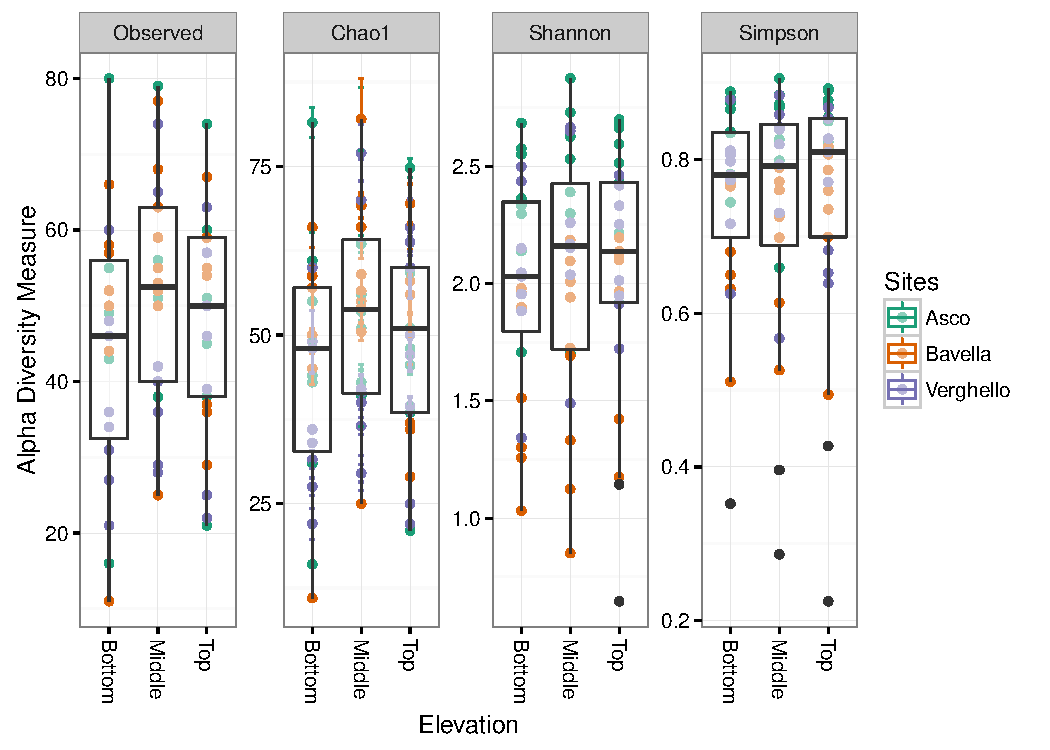
\includegraphics[width=\maxwidth]{figure/unnamed-chunk-41-1} 

}

\caption[Diversity in function of elevation]{Diversity in function of elevation. Color represent sites.}\label{fig:unnamed-chunk-41}
\end{figure}


\end{knitrout}

  \subsection{Which factor affect diversity?}
  
\begin{knitrout}\small
\definecolor{shadecolor}{rgb}{0.969, 0.969, 0.969}\color{fgcolor}\begin{kframe}
\begin{alltt}
\hlcom{## Uneven sequencing depth may have an impact}
\hlstd{readNumbers} \hlkwb{=} \hlkwd{apply}\hlstd{(}\hlkwd{t}\hlstd{(data.f3}\hlopt{@}\hlkwc{otu_table}\hlstd{),} \hlnum{1}\hlstd{, sum)}

\hlstd{otuHill} \hlkwb{<-} \hlkwd{renyi}\hlstd{(}\hlkwd{t}\hlstd{(data.f3}\hlopt{@}\hlkwc{otu_table}\hlstd{),} \hlkwc{scale} \hlstd{=} \hlkwd{c}\hlstd{(}\hlnum{0}\hlstd{,} \hlnum{1}\hlstd{,} \hlnum{2}\hlstd{),} \hlkwc{hill} \hlstd{= T)}

\hlstd{hill.1} \hlkwb{=} \hlstd{otuHill}\hlopt{$}\hlstr{"0"}
\hlstd{hill.2} \hlkwb{=} \hlstd{otuHill}\hlopt{$}\hlstr{"1"}
\hlstd{hill.3} \hlkwb{=} \hlstd{otuHill}\hlopt{$}\hlstr{"2"}

\hlstd{hill.1.m1} \hlkwb{=} \hlkwd{lm}\hlstd{(hill.1} \hlopt{~} \hlkwd{sqrt}\hlstd{(readNumbers)} \hlopt{+} \hlstd{data.f3}\hlopt{@}\hlkwc{sam_data}\hlopt{$}\hlstd{Sites} \hlopt{+}
                 \hlstd{data.f3}\hlopt{@}\hlkwc{sam_data}\hlopt{$}\hlstd{Age} \hlopt{+} \hlstd{data.f3}\hlopt{@}\hlkwc{sam_data}\hlopt{$}\hlstd{Elevation)}
\hlstd{hill.2.m1} \hlkwb{=} \hlkwd{lm}\hlstd{(hill.2} \hlopt{~} \hlkwd{sqrt}\hlstd{(readNumbers)} \hlopt{+} \hlstd{data.f3}\hlopt{@}\hlkwc{sam_data}\hlopt{$}\hlstd{Sites} \hlopt{+}
                 \hlstd{data.f3}\hlopt{@}\hlkwc{sam_data}\hlopt{$}\hlstd{Age} \hlopt{+} \hlstd{data.f3}\hlopt{@}\hlkwc{sam_data}\hlopt{$}\hlstd{Elevation)}
\hlstd{hill.3.m1} \hlkwb{=} \hlkwd{lm}\hlstd{(hill.3} \hlopt{~} \hlkwd{sqrt}\hlstd{(readNumbers)} \hlopt{+} \hlstd{data.f3}\hlopt{@}\hlkwc{sam_data}\hlopt{$}\hlstd{Sites} \hlopt{+}
                 \hlstd{data.f3}\hlopt{@}\hlkwc{sam_data}\hlopt{$}\hlstd{Age} \hlopt{+} \hlstd{data.f3}\hlopt{@}\hlkwc{sam_data}\hlopt{$}\hlstd{Elevation)}
\end{alltt}
\end{kframe}
\end{knitrout}

% latex table generated in R 3.3.1 by xtable 1.8-2 package
% Tue Jul 19 18:57:17 2016
\begin{table}[ht]
\centering
\begin{tabular}{lrrrr}
  \hline
 & Estimate & Std. Error & t value & Pr($>$$|$t$|$) \\ 
  \hline
(Intercept) & 29.4189474 & 133.5044144 & 0.2203594 & 0.8262927 \\ 
  sqrt(readNumbers) & 2.2375997 & 0.3396355 & 6.5882379 & 0.0000000 \\ 
  data.f3@sam\_data\$SitesBavella & -10.1118810 & 59.3953793 & -0.1702469 & 0.8653530 \\ 
  data.f3@sam\_data\$SitesVerghello & -84.7689405 & 59.4710379 & -1.4253819 & 0.1589059 \\ 
  data.f3@sam\_data\$AgeOld & -25.8215383 & 59.1438094 & -0.4365890 & 0.6638788 \\ 
  data.f3@sam\_data\$AgeYoung & -89.9361492 & 60.5620816 & -1.4850241 & 0.1424466 \\ 
  data.f3@sam\_data\$ElevationMiddle & 54.0275700 & 59.8951283 & 0.9020361 & 0.3704200 \\ 
  data.f3@sam\_data\$ElevationTop & -3.7752802 & 59.0829784 & -0.0638979 & 0.9492507 \\ 
   \hline
\end{tabular}
\caption{Summary of the linear model of species richness 
      (Hill number 1 (q = 0)} 
\end{table}


% latex table generated in R 3.3.1 by xtable 1.8-2 package
% Tue Jul 19 18:57:17 2016
\begin{table}[ht]
\centering
\begin{tabular}{lrrrr}
  \hline
 & Estimate & Std. Error & t value & Pr($>$$|$t$|$) \\ 
  \hline
(Intercept) & 13.8331728 & 8.1620095 & 1.6948244 & 0.0949697 \\ 
  sqrt(readNumbers) & 0.0784018 & 0.0207642 & 3.7758197 & 0.0003517 \\ 
  data.f3@sam\_data\$SitesBavella & -13.4455488 & 3.6312331 & -3.7027501 & 0.0004463 \\ 
  data.f3@sam\_data\$SitesVerghello & -4.3814745 & 3.6358586 & -1.2050729 & 0.2326122 \\ 
  data.f3@sam\_data\$AgeOld & -0.6822508 & 3.6158530 & -0.1886832 & 0.8509381 \\ 
  data.f3@sam\_data\$AgeYoung & -1.1411514 & 3.7025613 & -0.3082059 & 0.7589265 \\ 
  data.f3@sam\_data\$ElevationMiddle & 2.4734946 & 3.6617861 & 0.6754886 & 0.5017988 \\ 
  data.f3@sam\_data\$ElevationTop & -2.1846248 & 3.6121340 & -0.6048017 & 0.5474492 \\ 
   \hline
\end{tabular}
\caption{Summary of the linear model of the exponential of 
      Shannon’s entropy index (Hill number 2 (q = 1)} 
\end{table}


% latex table generated in R 3.3.1 by xtable 1.8-2 package
% Tue Jul 19 18:57:17 2016
\begin{table}[ht]
\centering
\begin{tabular}{lrrrr}
  \hline
 & Estimate & Std. Error & t value & Pr($>$$|$t$|$) \\ 
  \hline
(Intercept) & 6.7623603 & 3.4389473 & 1.9664042 & 0.0535919 \\ 
  sqrt(readNumbers) & 0.0321194 & 0.0087487 & 3.6713377 & 0.0004940 \\ 
  data.f3@sam\_data\$SitesBavella & -7.5793958 & 1.5299687 & -4.9539547 & 0.0000056 \\ 
  data.f3@sam\_data\$SitesVerghello & -2.3673181 & 1.5319176 & -1.5453299 & 0.1271973 \\ 
  data.f3@sam\_data\$AgeOld & -0.0838357 & 1.5234885 & -0.0550288 & 0.9562870 \\ 
  data.f3@sam\_data\$AgeYoung & 0.5107140 & 1.5600219 & 0.3273762 & 0.7444518 \\ 
  data.f3@sam\_data\$ElevationMiddle & 0.5160196 & 1.5428418 & 0.3344605 & 0.7391257 \\ 
  data.f3@sam\_data\$ElevationTop & -1.7834158 & 1.5219216 & -1.1718185 & 0.2456139 \\ 
   \hline
\end{tabular}
\caption{Summary of the linear model of inverse of Simpson’s
      concentration index (Hill number 3 (q = 2)} 
\end{table}


Post-hoc Tukey tests among the three experimental treatments with partial residuals, after accounting for differential sequencing success.
\begin{knitrout}\small
\definecolor{shadecolor}{rgb}{0.969, 0.969, 0.969}\color{fgcolor}\begin{kframe}
\begin{alltt}
\hlstd{tuk1} \hlkwb{<-} \hlkwd{TukeyHSD}\hlstd{(}\hlkwd{aov}\hlstd{(}\hlkwd{lm}\hlstd{(hill.1} \hlopt{~} \hlkwd{sqrt}\hlstd{(readNumbers))}\hlopt{$}\hlstd{residuals} \hlopt{~} \hlstd{data.f3}\hlopt{@}\hlkwc{sam_data}\hlopt{$}\hlstd{Site))}
\hlstd{tuk2} \hlkwb{<-} \hlkwd{TukeyHSD}\hlstd{(}\hlkwd{aov}\hlstd{(}\hlkwd{lm}\hlstd{(hill.2} \hlopt{~} \hlkwd{sqrt}\hlstd{(readNumbers))}\hlopt{$}\hlstd{residuals} \hlopt{~} \hlstd{data.f3}\hlopt{@}\hlkwc{sam_data}\hlopt{$}\hlstd{Site))}
\hlstd{tuk3} \hlkwb{<-} \hlkwd{TukeyHSD}\hlstd{(}\hlkwd{aov}\hlstd{(}\hlkwd{lm}\hlstd{(hill.3} \hlopt{~} \hlkwd{sqrt}\hlstd{(readNumbers))}\hlopt{$}\hlstd{residuals} \hlopt{~} \hlstd{data.f3}\hlopt{@}\hlkwc{sam_data}\hlopt{$}\hlstd{Site))}
\end{alltt}
\end{kframe}
\end{knitrout}



\begin{knitrout}\small
\definecolor{shadecolor}{rgb}{0.969, 0.969, 0.969}\color{fgcolor}\begin{kframe}
\begin{alltt}
\hlkwd{ggplot}\hlstd{(}\hlkwc{data} \hlstd{= df)} \hlopt{+} \hlkwd{geom_linerange}\hlstd{(}\hlkwd{aes}\hlstd{(}\hlkwc{ymax} \hlstd{= xSup,} \hlkwc{ymin} \hlstd{= xInf,} \hlkwc{x} \hlstd{= y),} \hlkwc{size} \hlstd{=} \hlnum{2}\hlstd{)} \hlopt{+}
  \hlkwd{geom_point}\hlstd{(}\hlkwd{aes}\hlstd{(}\hlkwc{x}\hlstd{=y,} \hlkwc{y}\hlstd{=x),} \hlkwc{size}\hlstd{=}\hlnum{4}\hlstd{,} \hlkwc{shape}\hlstd{=}\hlnum{21}\hlstd{,} \hlkwc{fill}\hlstd{=}\hlstr{"white"}\hlstd{)} \hlopt{+}
  \hlkwd{coord_flip}\hlstd{()} \hlopt{+} \hlkwd{theme_gray}\hlstd{()} \hlopt{+} \hlkwd{geom_hline}\hlstd{(}\hlkwc{yintercept} \hlstd{=} \hlnum{0}\hlstd{)} \hlopt{+}
  \hlkwd{ylab}\hlstd{(}\hlstr{"Differences in mean levels"}\hlstd{)} \hlopt{+} \hlkwd{xlab}\hlstd{(}\hlstr{""}\hlstd{)}
\end{alltt}
\end{kframe}\begin{figure}

{\centering 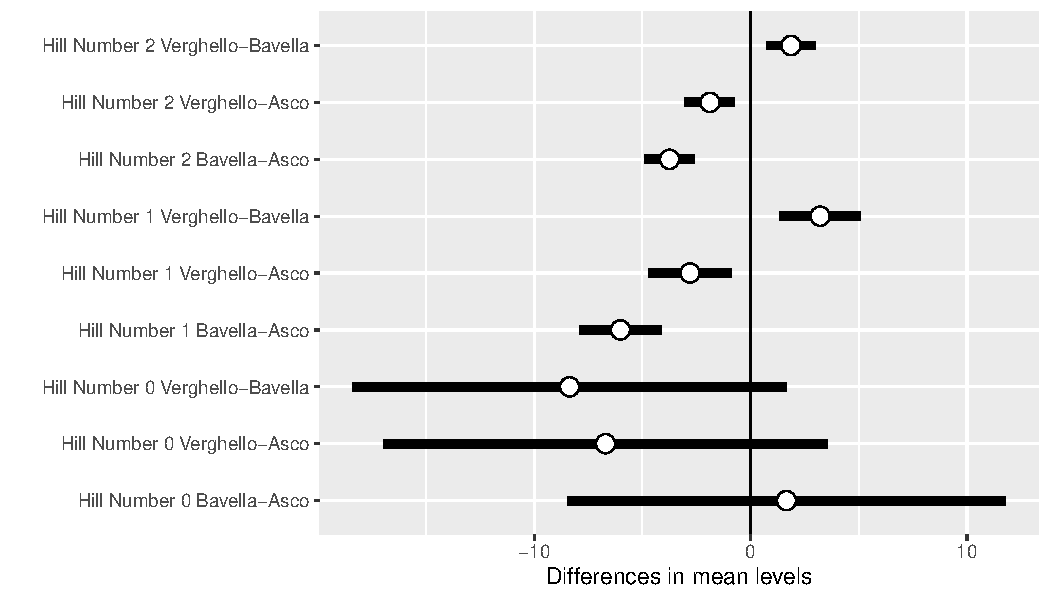
\includegraphics[width=\maxwidth]{figure/unnamed-chunk-47-1} 

}

\caption[Results of the Tuckey HSD testing for differences in mean Hill numbers among pairs of modalities]{Results of the Tuckey HSD testing for differences in mean Hill numbers among pairs of modalities}\label{fig:unnamed-chunk-47}
\end{figure}


\end{knitrout}


\section{Effect of site, age and elevation on fungal endophytic beta-diversity}

  \subsection{Venn diagramm}
  
\begin{knitrout}\small
\definecolor{shadecolor}{rgb}{0.969, 0.969, 0.969}\color{fgcolor}\begin{kframe}
\begin{alltt}
\hlkwd{venn_phyloseq}\hlstd{(data.f3,} \hlstr{"Sites"}\hlstd{,} \hlkwc{printValues} \hlstd{= F)}
\end{alltt}
\end{kframe}\begin{figure}

{\centering 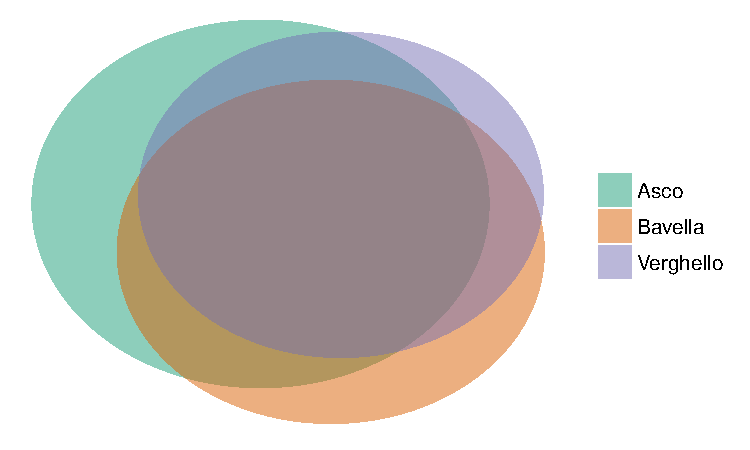
\includegraphics[width=\maxwidth]{figure/unnamed-chunk-48-1} 

}

\caption[Venn diagramm ef the distribution of OTUs among Sites]{Venn diagramm ef the distribution of OTUs among Sites}\label{fig:unnamed-chunk-48}
\end{figure}


\end{knitrout}

\begin{knitrout}\small
\definecolor{shadecolor}{rgb}{0.969, 0.969, 0.969}\color{fgcolor}\begin{kframe}
\begin{alltt}
\hlkwd{venn_phyloseq}\hlstd{(data.f3,} \hlstr{"Age"}\hlstd{,} \hlkwc{printValues} \hlstd{= F)}
\end{alltt}
\end{kframe}\begin{figure}

{\centering 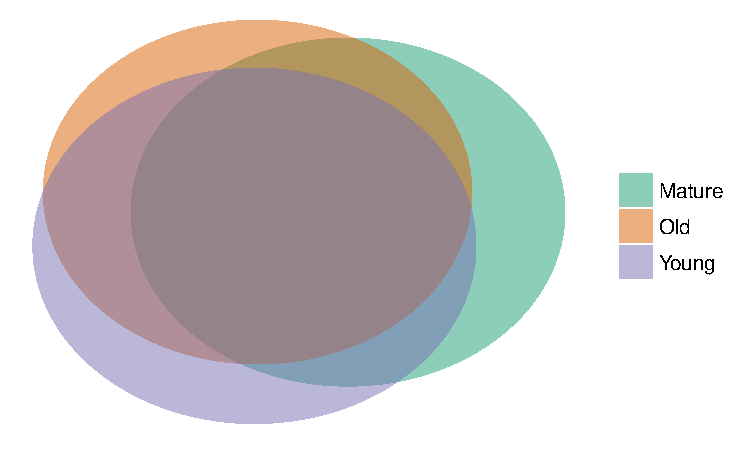
\includegraphics[width=\maxwidth]{figure/unnamed-chunk-49-1} 

}

\caption[Venn diagramm ef the distribution of OTUs among host age]{Venn diagramm ef the distribution of OTUs among host age}\label{fig:unnamed-chunk-49}
\end{figure}


\end{knitrout}

\begin{knitrout}\small
\definecolor{shadecolor}{rgb}{0.969, 0.969, 0.969}\color{fgcolor}\begin{kframe}
\begin{alltt}
\hlkwd{venn_phyloseq}\hlstd{(data.f3,} \hlstr{"Elevation"}\hlstd{,} \hlkwc{printValues} \hlstd{= F)}
\end{alltt}
\end{kframe}\begin{figure}

{\centering 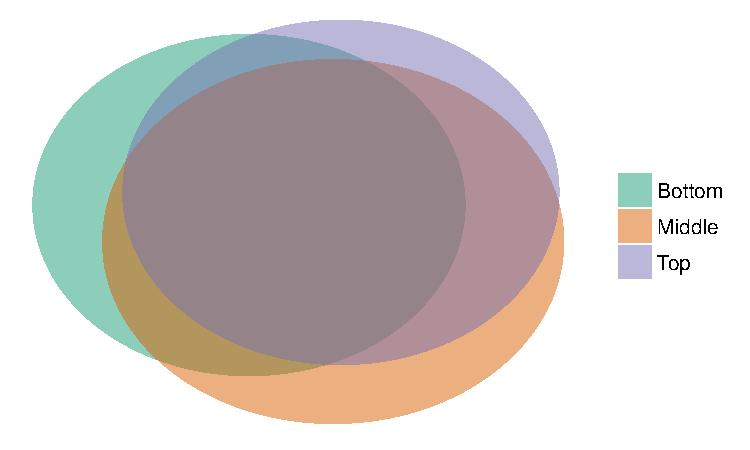
\includegraphics[width=\maxwidth]{figure/unnamed-chunk-50-1} 

}

\caption[Venn diagramm ef the distribution of OTUs among elevation of samples]{Venn diagramm ef the distribution of OTUs among elevation of samples}\label{fig:unnamed-chunk-50}
\end{figure}


\end{knitrout}


  \subsection{Ordination}

 Ordination of the OTUs table using NMDS (Non-metric MultiDimenstional Scaling).

\begin{knitrout}\small
\definecolor{shadecolor}{rgb}{0.969, 0.969, 0.969}\color{fgcolor}\begin{kframe}
\begin{alltt}
\hlstd{my.ord.nmds} \hlkwb{<-} \hlkwd{ordinate}\hlstd{(data.f3,} \hlkwc{method} \hlstd{=} \hlstr{"NMDS"}\hlstd{)}
\hlstd{my.ord.nmds}\hlopt{$}\hlstd{stress}
\end{alltt}
\end{kframe}
\end{knitrout}

\begin{knitrout}\small
\definecolor{shadecolor}{rgb}{0.969, 0.969, 0.969}\color{fgcolor}\begin{kframe}
\begin{alltt}
\hlkwd{stressplot}\hlstd{(my.ord.nmds)}
\end{alltt}
\end{kframe}\begin{figure}

{\centering 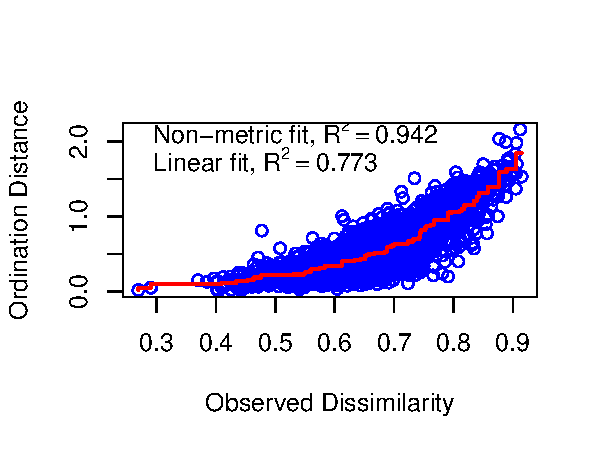
\includegraphics[width=\maxwidth]{figure/unnamed-chunk-52-1} 

}

\caption[Stress plot of the NMDS]{Stress plot of the NMDS}\label{fig:unnamed-chunk-52}
\end{figure}


\end{knitrout}


\begin{knitrout}\small
\definecolor{shadecolor}{rgb}{0.969, 0.969, 0.969}\color{fgcolor}\begin{kframe}
\begin{alltt}
\hlstd{p} \hlkwb{<-} \hlkwd{plot_ordination}\hlstd{(data.f3, my.ord.nmds,} \hlkwc{color} \hlstd{=} \hlstr{"Sites"}\hlstd{,} \hlkwc{shape} \hlstd{=} \hlstr{"Age"}\hlstd{)}
\hlstd{p} \hlopt{+} \hlkwd{geom_point}\hlstd{(}\hlkwc{size} \hlstd{=} \hlnum{0}\hlstd{)} \hlopt{+}
  \hlkwd{geom_text}\hlstd{(}\hlkwd{aes}\hlstd{(}\hlkwc{x} \hlstd{= p}\hlopt{$}\hlstd{data}\hlopt{$}\hlstd{NMDS1,} \hlkwc{y} \hlstd{= p}\hlopt{$}\hlstd{data}\hlopt{$}\hlstd{NMDS2,}
                \hlkwc{label} \hlstd{=} \hlkwd{as.character}\hlstd{(}\hlkwd{as.vector}\hlstd{(data.f3}\hlopt{@}\hlkwc{sam_data}\hlstd{[,} \hlstr{"CODE"}\hlstd{]}\hlopt{$}\hlstd{CODE))))}
\end{alltt}
\end{kframe}\begin{figure}

{\centering 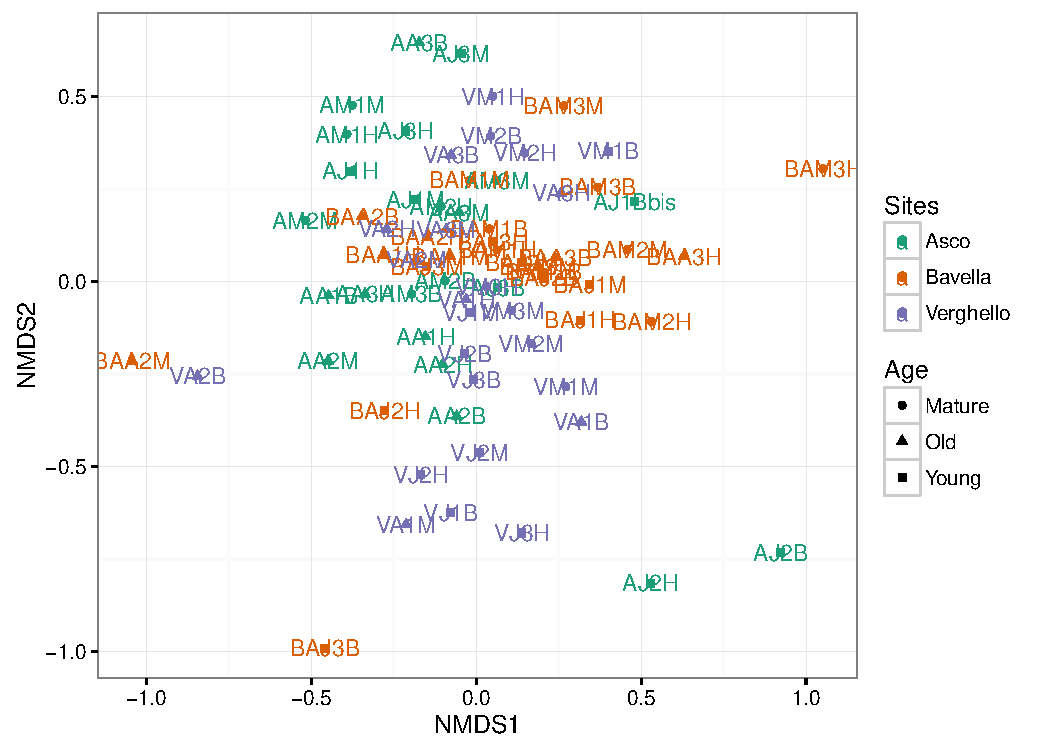
\includegraphics[width=\maxwidth]{figure/unnamed-chunk-53-1} 

}

\caption[NMDS of OTU table]{NMDS of OTU table. Colors represent sites and shape the age of tree.}\label{fig:unnamed-chunk-53}
\end{figure}


\end{knitrout}


\begin{knitrout}\small
\definecolor{shadecolor}{rgb}{0.969, 0.969, 0.969}\color{fgcolor}\begin{kframe}
\begin{alltt}
\hlstd{my.ord.nmds_gower} \hlkwb{<-} \hlkwd{ordinate}\hlstd{(data.f3,} \hlkwc{distance} \hlstd{=} \hlstr{"gower"}\hlstd{,}  \hlkwc{method} \hlstd{=} \hlstr{"NMDS"}\hlstd{)}
\end{alltt}
\begin{verbatim}
## Square root transformation
## Wisconsin double standardization
## Run 0 stress 0.2076191 
## Run 1 stress 0.2123561 
## Run 2 stress 0.2121729 
## Run 3 stress 0.2130255 
## Run 4 stress 0.2083093 
## Run 5 stress 0.2121839 
## Run 6 stress 0.2084524 
## Run 7 stress 0.2117324 
## Run 8 stress 0.2090304 
## Run 9 stress 0.2117702 
## Run 10 stress 0.2096642 
## Run 11 stress 0.2130115 
## Run 12 stress 0.2118757 
## Run 13 stress 0.2116805 
## Run 14 stress 0.2095071 
## Run 15 stress 0.2122905 
## Run 16 stress 0.2255298 
## Run 17 stress 0.2117692 
## Run 18 stress 0.2074187 
## ... New best solution
## ... Procrustes: rmse 0.0144286  max resid 0.08090176 
## Run 19 stress 0.2074905 
## ... Procrustes: rmse 0.04257561  max resid 0.1669314 
## Run 20 stress 0.2135174 
## *** No convergence -- monoMDS stopping criteria:
##      4: no. of iterations >= maxit
##     16: stress ratio > sratmax
\end{verbatim}
\begin{alltt}
\hlstd{my.ord.PCoA} \hlkwb{<-} \hlkwd{ordinate}\hlstd{(data.f3,} \hlkwc{method} \hlstd{=} \hlstr{"PCoA"}\hlstd{)}
\hlstd{my.ord.PCoA_gower} \hlkwb{<-} \hlkwd{ordinate}\hlstd{(data.f3,} \hlkwc{distance} \hlstd{=} \hlstr{"gower"}\hlstd{,} \hlkwc{method} \hlstd{=} \hlstr{"PCoA"}\hlstd{)}
\hlstd{my.ord.DCA} \hlkwb{<-} \hlkwd{ordinate}\hlstd{(data.f3,} \hlkwc{method} \hlstd{=} \hlstr{"DCA"}\hlstd{)}
\hlstd{my.ord.DCA_gower} \hlkwb{<-} \hlkwd{ordinate}\hlstd{(data.f3,} \hlkwc{distance} \hlstd{=} \hlstr{"gower"}\hlstd{,} \hlkwc{method} \hlstd{=} \hlstr{"DCA"}\hlstd{)}

\hlstd{p_NMDS_BRAY} \hlkwb{<-} \hlkwd{plot_ordination}\hlstd{(data.f3, my.ord.nmds,} \hlkwc{color} \hlstd{=} \hlstr{"Sites"}\hlstd{,}
                               \hlkwc{shape} \hlstd{=} \hlstr{"Age"}\hlstd{,} \hlkwc{label} \hlstd{=} \hlstr{"CODE"}\hlstd{)} \hlopt{+} \hlkwd{geom_point}\hlstd{(}\hlkwc{size} \hlstd{=} \hlnum{5}\hlstd{)}
\hlstd{p_NMDS_GOWER} \hlkwb{<-} \hlkwd{plot_ordination}\hlstd{(data.f3, my.ord.nmds_gower,} \hlkwc{color} \hlstd{=} \hlstr{"Sites"}\hlstd{,}
                                \hlkwc{shape} \hlstd{=} \hlstr{"Age"}\hlstd{,} \hlkwc{label} \hlstd{=} \hlstr{"CODE"}\hlstd{)} \hlopt{+} \hlkwd{geom_point}\hlstd{(}\hlkwc{size} \hlstd{=} \hlnum{5}\hlstd{)}
\hlstd{p_PCoA_BRAY} \hlkwb{<-} \hlkwd{plot_ordination}\hlstd{(data.f3, my.ord.PCoA,} \hlkwc{color} \hlstd{=} \hlstr{"Sites"}\hlstd{,}
                               \hlkwc{shape} \hlstd{=} \hlstr{"Age"}\hlstd{,} \hlkwc{label} \hlstd{=} \hlstr{"CODE"}\hlstd{)} \hlopt{+} \hlkwd{geom_point}\hlstd{(}\hlkwc{size} \hlstd{=} \hlnum{5}\hlstd{)}
\hlstd{p_PCoA_GOWER} \hlkwb{<-} \hlkwd{plot_ordination}\hlstd{(data.f3, my.ord.PCoA_gower,} \hlkwc{color} \hlstd{=} \hlstr{"Sites"}\hlstd{,}
                                \hlkwc{shape} \hlstd{=} \hlstr{"Age"}\hlstd{,} \hlkwc{label} \hlstd{=} \hlstr{"CODE"}\hlstd{)} \hlopt{+} \hlkwd{geom_point}\hlstd{(}\hlkwc{size} \hlstd{=} \hlnum{5}\hlstd{)}
\hlstd{p_DCA_BRAY} \hlkwb{<-} \hlkwd{plot_ordination}\hlstd{(data.f3, my.ord.DCA,} \hlkwc{color} \hlstd{=} \hlstr{"Sites"}\hlstd{,}
                              \hlkwc{shape} \hlstd{=} \hlstr{"Age"}\hlstd{,} \hlkwc{label} \hlstd{=} \hlstr{"CODE"}\hlstd{)} \hlopt{+} \hlkwd{geom_point}\hlstd{(}\hlkwc{size} \hlstd{=} \hlnum{5}\hlstd{)}
\hlstd{p_DCA_GOWER} \hlkwb{<-} \hlkwd{plot_ordination}\hlstd{(data.f3, my.ord.DCA_gower,} \hlkwc{color} \hlstd{=} \hlstr{"Sites"}\hlstd{,}
                               \hlkwc{shape} \hlstd{=} \hlstr{"Age"}\hlstd{,} \hlkwc{label} \hlstd{=} \hlstr{"CODE"}\hlstd{)} \hlopt{+} \hlkwd{geom_point}\hlstd{(}\hlkwc{size} \hlstd{=} \hlnum{5}\hlstd{)}
\end{alltt}
\end{kframe}
\end{knitrout}

\begin{landscape}
\begin{knitrout}\small
\definecolor{shadecolor}{rgb}{0.969, 0.969, 0.969}\color{fgcolor}\begin{kframe}
\begin{alltt}
\hlkwd{multiplot}\hlstd{(p_NMDS_BRAY, p_NMDS_GOWER, p_PCoA_BRAY, p_PCoA_GOWER, p_DCA_BRAY, p_DCA_GOWER,}
          \hlkwc{cols} \hlstd{=} \hlnum{3}\hlstd{)}
\end{alltt}
\end{kframe}\begin{figure}

{\centering 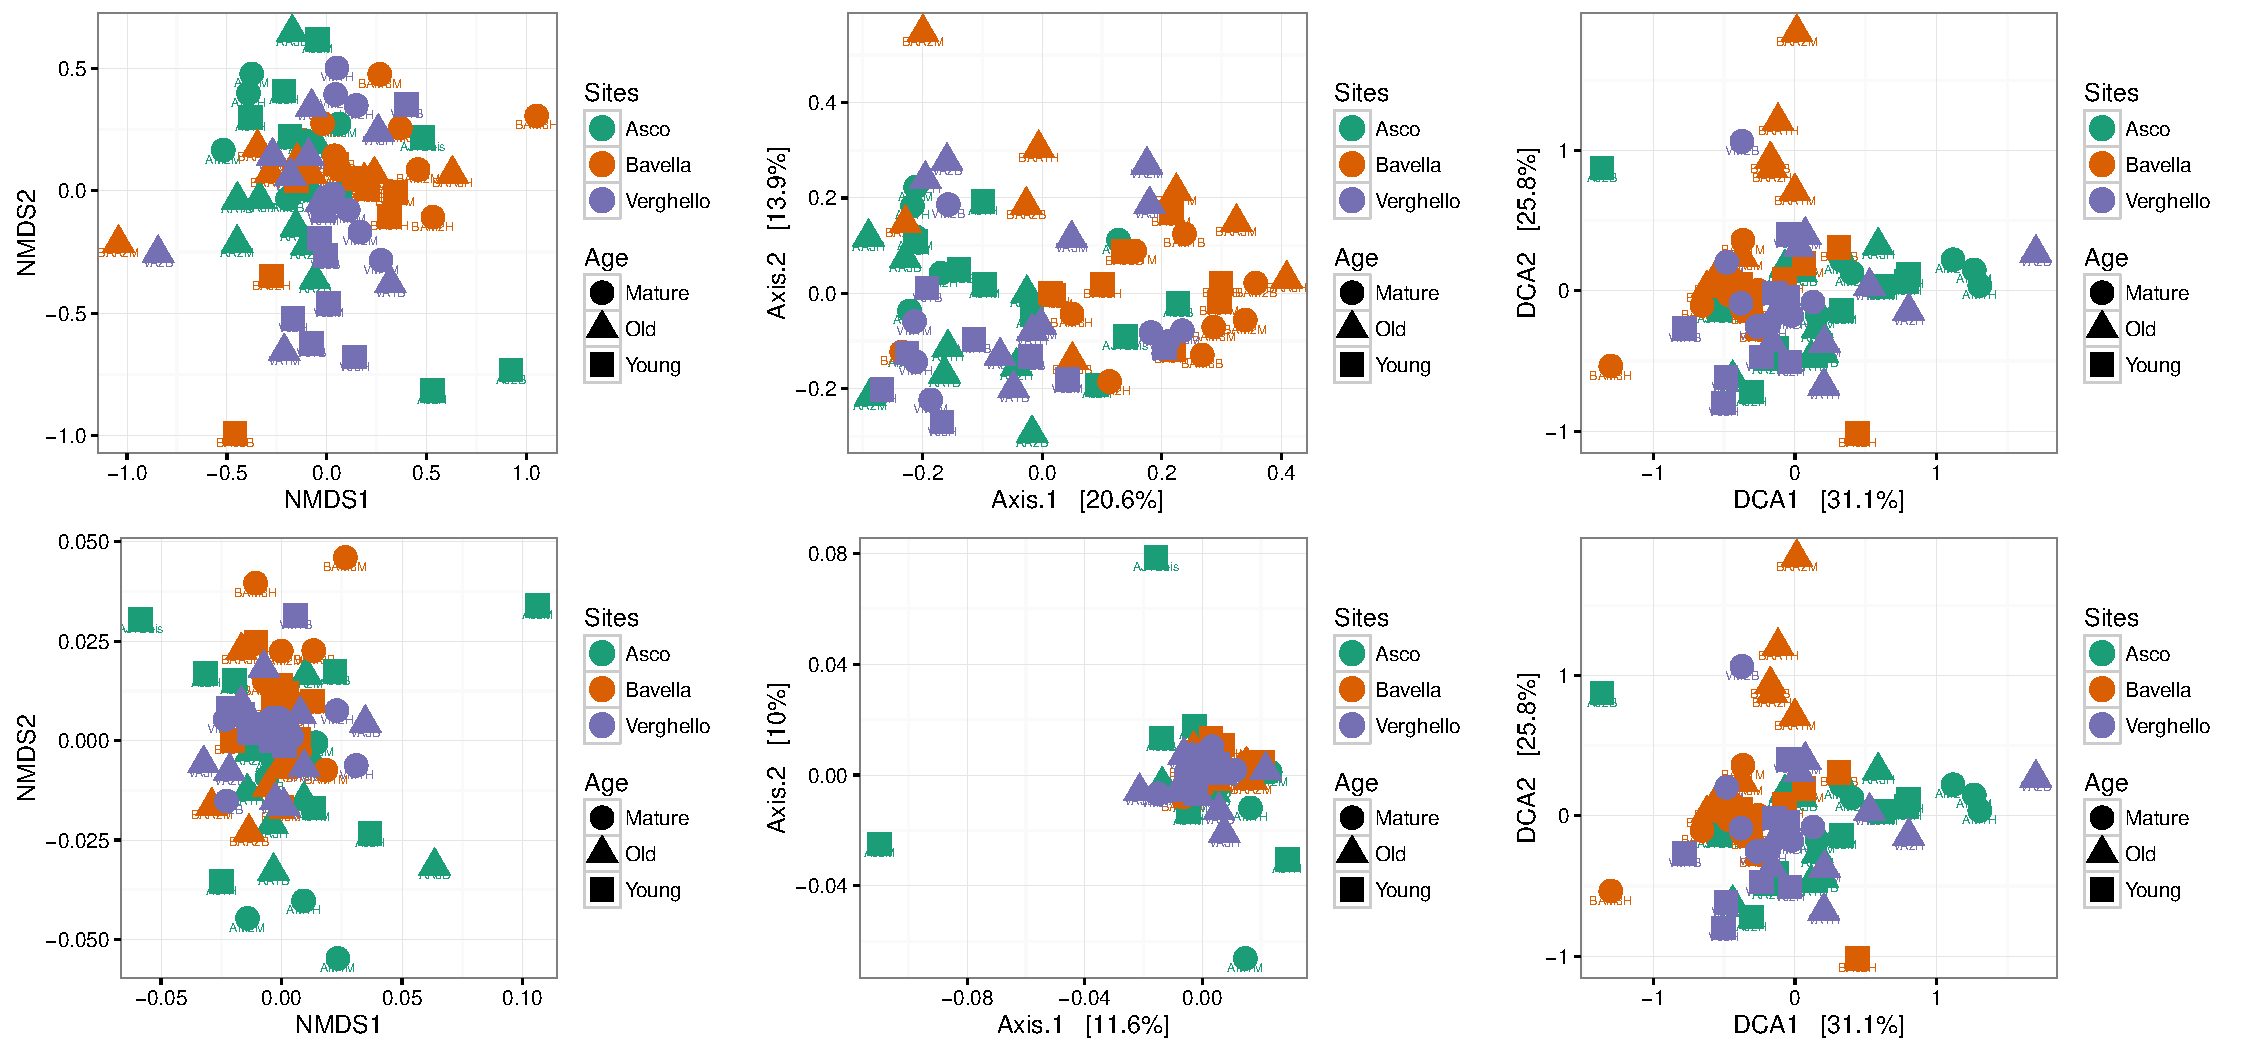
\includegraphics[width=\maxwidth]{figure/unnamed-chunk-55-1} 

}

\caption[Comparison of different distances (bray (up) and gower (bottom)) and ordination methods (NMDS (left), PCoA (center) and DCA (right))]{Comparison of different distances (bray (up) and gower (bottom)) and ordination methods (NMDS (left), PCoA (center) and DCA (right)).}\label{fig:unnamed-chunk-55}
\end{figure}


\end{knitrout}
\end{landscape}

  \subsection{Permanova on sites, host ages and elevation}
  
\begin{knitrout}\small
\definecolor{shadecolor}{rgb}{0.969, 0.969, 0.969}\color{fgcolor}\begin{kframe}
\begin{alltt}
\hlstd{sam_data} \hlkwb{<-} \hlkwd{as.data.frame}\hlstd{(}\hlkwd{unclass}\hlstd{(data.f3}\hlopt{@}\hlkwc{sam_data}\hlstd{))}
\hlstd{sam_data}\hlopt{$}\hlstd{IndividualTree} \hlkwb{<-} \hlkwd{paste}\hlstd{(sam_data}\hlopt{$}\hlstd{Sites, sam_data}\hlopt{$}\hlstd{Age, sam_data}\hlopt{$}\hlstd{Tree)}
\hlstd{res.ado} \hlkwb{<-} \hlkwd{adonis}\hlstd{(}\hlkwd{t}\hlstd{(data.f3}\hlopt{@}\hlkwc{otu_table}\hlstd{)} \hlopt{~}  \hlstd{Sites} \hlopt{*} \hlstd{Age} \hlopt{*} \hlstd{Elevation, sam_data,}
                  \hlkwc{permutation} \hlstd{=} \hlnum{9999}\hlstd{)}
\end{alltt}
\end{kframe}
\end{knitrout}

If we only keep the 593 OTUs present in more than 30 sample, the Permanova results is the following:
\begin{knitrout}\small
\definecolor{shadecolor}{rgb}{0.969, 0.969, 0.969}\color{fgcolor}\begin{kframe}
\begin{alltt}
\hlstd{res.ado_sampMin30} \hlkwb{<-} \hlkwd{adonis}\hlstd{(}\hlkwd{t}\hlstd{(data.f3}\hlopt{@}\hlkwc{otu_table}\hlstd{[}\hlkwd{rowSums}\hlstd{(data.f3}\hlopt{@}\hlkwc{otu_table}\hlopt{>}\hlnum{0}\hlstd{)}\hlopt{>=}\hlnum{30}\hlstd{,])} \hlopt{~}
                              \hlstd{Sites} \hlopt{*} \hlstd{Age} \hlopt{*} \hlstd{Elevation, sam_data,} \hlkwc{permutation} \hlstd{=} \hlnum{9999}\hlstd{)}
\end{alltt}
\end{kframe}
\end{knitrout}

\begin{kframe}
\begin{alltt}
\hlkwd{xtable}\hlstd{(res.ado}\hlopt{$}\hlstd{aov.tab,} \hlkwc{caption} \hlstd{=} \hlstr{"Result of the permanova on abundances 
       (number of sequence)."}\hlstd{)}
\end{alltt}
\end{kframe}% latex table generated in R 3.3.1 by xtable 1.8-2 package
% Tue Jul 19 18:57:38 2016
\begin{table}[ht]
\centering
\begin{tabular}{lrrrrrr}
  \hline
 & Df & SumsOfSqs & MeanSqs & F.Model & R2 & Pr($>$F) \\ 
  \hline
Sites & 2 & 2.05 & 1.02 & 4.52 & 0.11 & 0.0001 \\ 
  Age & 2 & 0.71 & 0.35 & 1.56 & 0.04 & 0.0374 \\ 
  Elevation & 2 & 0.60 & 0.30 & 1.33 & 0.03 & 0.1125 \\ 
  Sites:Age & 4 & 1.67 & 0.42 & 1.84 & 0.09 & 0.0007 \\ 
  Sites:Elevation & 4 & 0.90 & 0.22 & 0.99 & 0.05 & 0.4788 \\ 
  Age:Elevation & 4 & 1.15 & 0.29 & 1.27 & 0.06 & 0.0896 \\ 
  Sites:Age:Elevation & 8 & 1.96 & 0.25 & 1.09 & 0.10 & 0.2564 \\ 
  Residuals & 45 & 10.18 & 0.23 &  & 0.53 &  \\ 
  Total & 71 & 19.21 &  &  & 1.00 &  \\ 
   \hline
\end{tabular}
\caption{Result of the permanova on abundances 
       (number of sequence).} 
\end{table}


\begin{kframe}
\begin{alltt}
\hlkwd{xtable}\hlstd{(res.ado_sampMin30}\hlopt{$}\hlstd{aov.tab,} \hlkwc{caption} \hlstd{=} \hlstr{"Result of the permanova on abundances 
       (number of sequence) using only OTUs present in more than 30 samples"}\hlstd{)}
\end{alltt}
\end{kframe}% latex table generated in R 3.3.1 by xtable 1.8-2 package
% Tue Jul 19 18:57:38 2016
\begin{table}[ht]
\centering
\begin{tabular}{lrrrrrr}
  \hline
 & Df & SumsOfSqs & MeanSqs & F.Model & R2 & Pr($>$F) \\ 
  \hline
Sites & 2 & 2.01 & 1.00 & 4.69 & 0.11 & 0.0001 \\ 
  Age & 2 & 0.68 & 0.34 & 1.59 & 0.04 & 0.0371 \\ 
  Elevation & 2 & 0.59 & 0.29 & 1.37 & 0.03 & 0.1076 \\ 
  Sites:Age & 4 & 1.63 & 0.41 & 1.90 & 0.09 & 0.0011 \\ 
  Sites:Elevation & 4 & 0.86 & 0.21 & 1.00 & 0.05 & 0.4508 \\ 
  Age:Elevation & 4 & 1.12 & 0.28 & 1.30 & 0.06 & 0.0833 \\ 
  Sites:Age:Elevation & 8 & 1.87 & 0.23 & 1.09 & 0.10 & 0.2652 \\ 
  Residuals & 45 & 9.63 & 0.21 &  & 0.52 &  \\ 
  Total & 71 & 18.38 &  &  & 1.00 &  \\ 
   \hline
\end{tabular}
\caption{Result of the permanova on abundances 
       (number of sequence) using only OTUs present in more than 30 samples} 
\end{table}


\begin{knitrout}\small
\definecolor{shadecolor}{rgb}{0.969, 0.969, 0.969}\color{fgcolor}\begin{kframe}
\begin{alltt}
\hlstd{res.ado_bin} \hlkwb{<-} \hlkwd{adonis}\hlstd{(}\hlkwd{t}\hlstd{(}\hlkwd{as.binaryOtuTable}\hlstd{(data.f3)}\hlopt{@}\hlkwc{otu_table}\hlstd{)} \hlopt{~}  \hlstd{Sites} \hlopt{*} \hlstd{Age} \hlopt{*}
                        \hlstd{Elevation, sam_data,} \hlkwc{permutation} \hlstd{=} \hlnum{9999}\hlstd{)}
\end{alltt}
\end{kframe}
\end{knitrout}

\begin{kframe}
\begin{alltt}
\hlkwd{xtable}\hlstd{(res.ado_bin}\hlopt{$}\hlstd{aov.tab,} \hlkwc{caption} \hlstd{=} \hlstr{"Result of the permanova on OTUs
       (each OTU is representing by one sequence))."}\hlstd{)}
\end{alltt}
\end{kframe}% latex table generated in R 3.3.1 by xtable 1.8-2 package
% Tue Jul 19 18:57:42 2016
\begin{table}[ht]
\centering
\begin{tabular}{lrrrrrr}
  \hline
 & Df & SumsOfSqs & MeanSqs & F.Model & R2 & Pr($>$F) \\ 
  \hline
Sites & 2 & 1.05 & 0.52 & 3.72 & 0.09 & 0.0001 \\ 
  Age & 2 & 0.45 & 0.22 & 1.58 & 0.04 & 0.0080 \\ 
  Elevation & 2 & 0.29 & 0.15 & 1.04 & 0.03 & 0.3762 \\ 
  Sites:Age & 4 & 0.84 & 0.21 & 1.49 & 0.08 & 0.0031 \\ 
  Sites:Elevation & 4 & 0.48 & 0.12 & 0.84 & 0.04 & 0.8951 \\ 
  Age:Elevation & 4 & 0.58 & 0.14 & 1.02 & 0.05 & 0.4031 \\ 
  Sites:Age:Elevation & 8 & 1.06 & 0.13 & 0.94 & 0.10 & 0.7012 \\ 
  Residuals & 45 & 6.35 & 0.14 &  & 0.57 &  \\ 
  Total & 71 & 11.09 &  &  & 1.00 &  \\ 
   \hline
\end{tabular}
\caption{Result of the permanova on OTUs
       (each OTU is representing by one sequence)).} 
\end{table}



  \subsection{Permanova on sites, host ages and individual trees}
  
\begin{knitrout}\small
\definecolor{shadecolor}{rgb}{0.969, 0.969, 0.969}\color{fgcolor}\begin{kframe}
\begin{alltt}
\hlstd{res.ado_Tree} \hlkwb{<-} \hlkwd{adonis}\hlstd{(}\hlkwd{t}\hlstd{(data.f3}\hlopt{@}\hlkwc{otu_table}\hlstd{)} \hlopt{~}   \hlstd{Sites}\hlopt{*}\hlstd{Age} \hlopt{+} \hlstd{Sites}\hlopt{:}\hlstd{Age}\hlopt{:}\hlstd{IndividualTree ,}
                       \hlstd{sam_data,} \hlkwc{permutation} \hlstd{=} \hlnum{9999}\hlstd{)}
\hlstd{res.ado_Tree_sampMin30} \hlkwb{<-} \hlkwd{adonis}\hlstd{(}\hlkwd{t}\hlstd{(data.f3}\hlopt{@}\hlkwc{otu_table}\hlstd{[}\hlkwd{rowSums}\hlstd{(data.f3}\hlopt{@}\hlkwc{otu_table}\hlopt{>}\hlnum{0}\hlstd{)}\hlopt{>=}\hlnum{30}\hlstd{,])} \hlopt{~}
                                   \hlstd{Sites}\hlopt{*}\hlstd{Age} \hlopt{+} \hlstd{Sites}\hlopt{:}\hlstd{Age}\hlopt{:}\hlstd{IndividualTree , sam_data,}
                                 \hlkwc{permutation} \hlstd{=} \hlnum{9999}\hlstd{)}
\hlstd{res.ado_Tree_bin} \hlkwb{<-} \hlkwd{adonis}\hlstd{(}\hlkwd{t}\hlstd{(}\hlkwd{as.binaryOtuTable}\hlstd{(data.f3)}\hlopt{@}\hlkwc{otu_table}\hlstd{)} \hlopt{~}
                             \hlstd{Sites}\hlopt{*}\hlstd{Age} \hlopt{+} \hlstd{Sites}\hlopt{:}\hlstd{Age}\hlopt{:}\hlstd{IndividualTree , sam_data,}
                           \hlkwc{permutation} \hlstd{=} \hlnum{9999}\hlstd{)}
\end{alltt}
\end{kframe}
\end{knitrout}

\begin{kframe}
\begin{alltt}
\hlkwd{xtable}\hlstd{(res.ado_Tree}\hlopt{$}\hlstd{aov.tab,} \hlkwc{caption} \hlstd{=} \hlstr{"Result of the permanova on abundances 
       (number of sequence)."}\hlstd{)}
\end{alltt}
\end{kframe}% latex table generated in R 3.3.1 by xtable 1.8-2 package
% Tue Jul 19 18:57:50 2016
\begin{table}[ht]
\centering
\begin{tabular}{lrrrrrr}
  \hline
 & Df & SumsOfSqs & MeanSqs & F.Model & R2 & Pr($>$F) \\ 
  \hline
Sites & 2 & 2.05 & 1.02 & 4.91 & 0.11 & 0.0001 \\ 
  Age & 2 & 0.71 & 0.35 & 1.69 & 0.04 & 0.0209 \\ 
  Sites:Age & 4 & 1.68 & 0.42 & 2.02 & 0.09 & 0.0003 \\ 
  Sites:Age:IndividualTree & 18 & 5.40 & 0.30 & 1.44 & 0.28 & 0.0004 \\ 
  Residuals & 45 & 9.38 & 0.21 &  & 0.49 &  \\ 
  Total & 71 & 19.21 &  &  & 1.00 &  \\ 
   \hline
\end{tabular}
\caption{Result of the permanova on abundances 
       (number of sequence).} 
\end{table}


\begin{kframe}
\begin{alltt}
\hlkwd{xtable}\hlstd{(res.ado_Tree_sampMin30}\hlopt{$}\hlstd{aov.tab,} \hlkwc{caption} \hlstd{=} \hlstr{"Result of the permanova on abundances 
       (number of sequence) using only OTUs present in more than 30 samples"}\hlstd{)}
\end{alltt}
\end{kframe}% latex table generated in R 3.3.1 by xtable 1.8-2 package
% Tue Jul 19 18:57:50 2016
\begin{table}[ht]
\centering
\begin{tabular}{lrrrrrr}
  \hline
 & Df & SumsOfSqs & MeanSqs & F.Model & R2 & Pr($>$F) \\ 
  \hline
Sites & 2 & 2.01 & 1.00 & 5.10 & 0.11 & 0.0001 \\ 
  Age & 2 & 0.68 & 0.34 & 1.73 & 0.04 & 0.0212 \\ 
  Sites:Age & 4 & 1.64 & 0.41 & 2.09 & 0.09 & 0.0001 \\ 
  Sites:Age:IndividualTree & 18 & 5.20 & 0.29 & 1.47 & 0.28 & 0.0002 \\ 
  Residuals & 45 & 8.85 & 0.20 &  & 0.48 &  \\ 
  Total & 71 & 18.38 &  &  & 1.00 &  \\ 
   \hline
\end{tabular}
\caption{Result of the permanova on abundances 
       (number of sequence) using only OTUs present in more than 30 samples} 
\end{table}


\begin{kframe}
\begin{alltt}
\hlkwd{xtable}\hlstd{(res.ado_Tree_bin}\hlopt{$}\hlstd{aov.tab,} \hlkwc{caption} \hlstd{=} \hlstr{"Result of the permanova on OTUs
       (each OTU is representing by one sequence))."}\hlstd{)}
\end{alltt}
\end{kframe}% latex table generated in R 3.3.1 by xtable 1.8-2 package
% Tue Jul 19 18:57:50 2016
\begin{table}[ht]
\centering
\begin{tabular}{lrrrrrr}
  \hline
 & Df & SumsOfSqs & MeanSqs & F.Model & R2 & Pr($>$F) \\ 
  \hline
Sites & 2 & 1.05 & 0.52 & 4.18 & 0.09 & 0.0001 \\ 
  Age & 2 & 0.45 & 0.22 & 1.78 & 0.04 & 0.0013 \\ 
  Sites:Age & 4 & 0.85 & 0.21 & 1.70 & 0.08 & 0.0001 \\ 
  Sites:Age:IndividualTree & 18 & 3.10 & 0.17 & 1.37 & 0.28 & 0.0001 \\ 
  Residuals & 45 & 5.65 & 0.13 &  & 0.51 &  \\ 
  Total & 71 & 11.09 &  &  & 1.00 &  \\ 
   \hline
\end{tabular}
\caption{Result of the permanova on OTUs
       (each OTU is representing by one sequence)).} 
\end{table}


   \subsection{Differences in abundances and OTUs number by Order.}

\begin{landscape}
\begin{knitrout}\small
\definecolor{shadecolor}{rgb}{0.969, 0.969, 0.969}\color{fgcolor}\begin{kframe}
\begin{alltt}
\hlstd{data.f3_taxo_known} \hlkwb{<-} \hlkwd{prune_taxa}\hlstd{(}\hlkwd{taxa_names}\hlstd{(data.f3}\hlopt{@}\hlkwc{tax_table}\hlstd{)}
          \hlstd{[}\hlopt{!}\hlstd{(data.f3}\hlopt{@}\hlkwc{tax_table}\hlstd{[,} \hlnum{4}\hlstd{]} \hlopt \hlkwd{c}\hlstd{(}\hlstr{"unidentified"}\hlstd{,} \hlstr{"Incertae sedis"}\hlstd{))], data.f3)}
\hlstd{p} \hlkwb{<-} \hlkwd{plot_bar}\hlstd{(data.f3_taxo_known,} \hlstr{"Order"}\hlstd{,} \hlkwc{fill} \hlstd{=} \hlstr{"Class"}\hlstd{,} \hlkwc{facet_grid} \hlstd{= Age} \hlopt{~} \hlstd{Sites)}
\hlstd{p} \hlopt{+} \hlkwd{geom_bar}\hlstd{(}\hlkwd{aes}\hlstd{(}\hlkwc{color} \hlstd{= Class,} \hlkwc{fill} \hlstd{= Class),} \hlkwc{stat} \hlstd{=} \hlstr{"identity"}\hlstd{,} \hlkwc{position} \hlstd{=} \hlstr{"stack"}\hlstd{)}
\end{alltt}
\end{kframe}\begin{figure}

{\centering 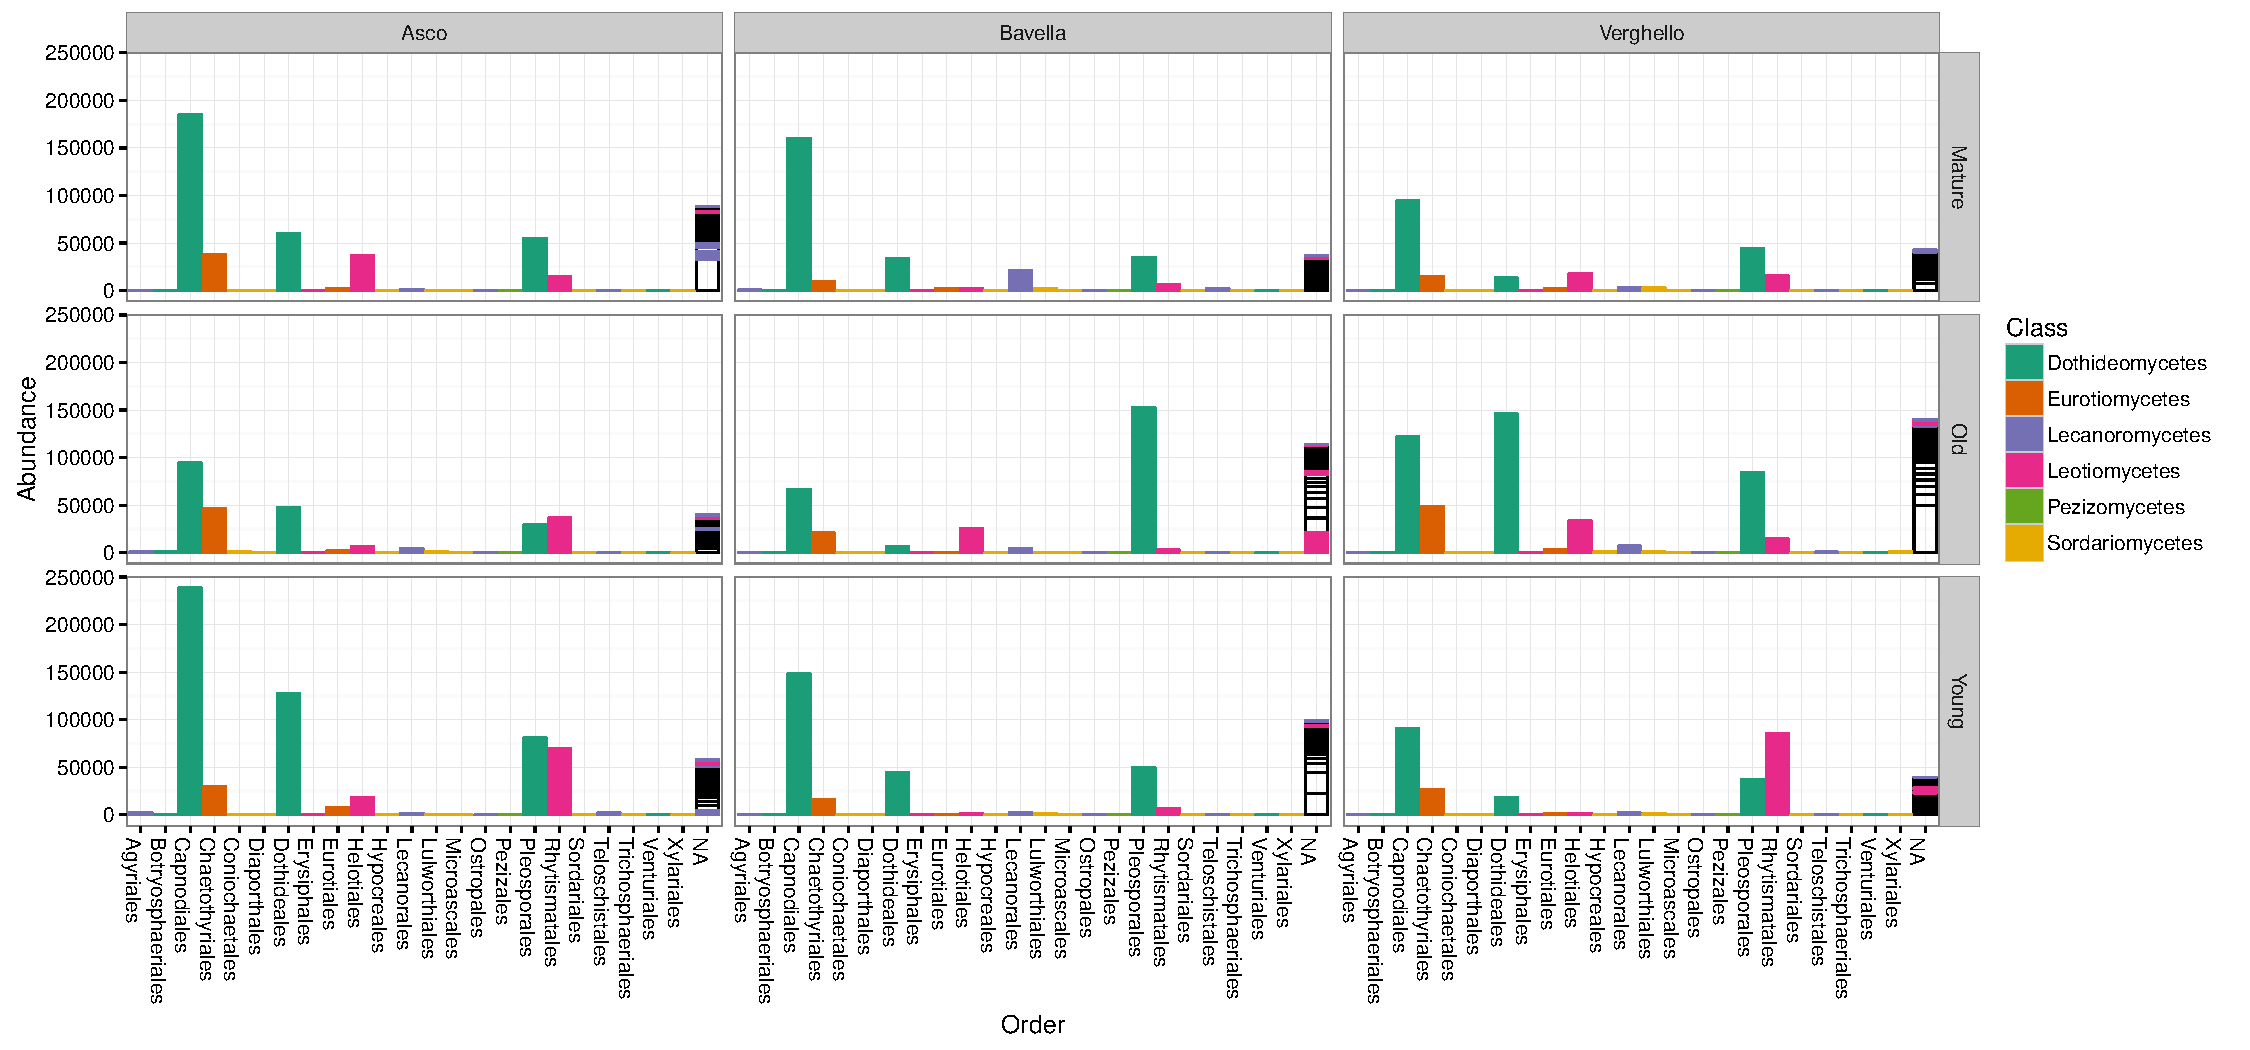
\includegraphics[width=\maxwidth]{figure/unnamed-chunk-66-1} 

}

\caption[Taxonomic distribution of sequences in the different site * age combinaison]{Taxonomic distribution of sequences in the different site * age combinaison.}\label{fig:unnamed-chunk-66}
\end{figure}


\end{knitrout}
\end{landscape}

\begin{landscape}
\begin{knitrout}\small
\definecolor{shadecolor}{rgb}{0.969, 0.969, 0.969}\color{fgcolor}\begin{kframe}
\begin{alltt}
\hlstd{p} \hlkwb{<-} \hlkwd{plot_bar}\hlstd{(}\hlkwd{as.binaryOtuTable}\hlstd{(data.f3_taxo_known),} \hlstr{"Order"}\hlstd{,} \hlkwc{fill} \hlstd{=} \hlstr{"Class"}\hlstd{,}
              \hlkwc{facet_grid} \hlstd{= Age} \hlopt{~} \hlstd{Sites)}
\hlstd{p} \hlopt{+} \hlkwd{geom_bar}\hlstd{(}\hlkwd{aes}\hlstd{(}\hlkwc{color} \hlstd{= Class,} \hlkwc{fill} \hlstd{= Class),} \hlkwc{stat} \hlstd{=} \hlstr{"identity"}\hlstd{,} \hlkwc{position} \hlstd{=} \hlstr{"stack"}\hlstd{)}
\end{alltt}
\end{kframe}\begin{figure}

{\centering 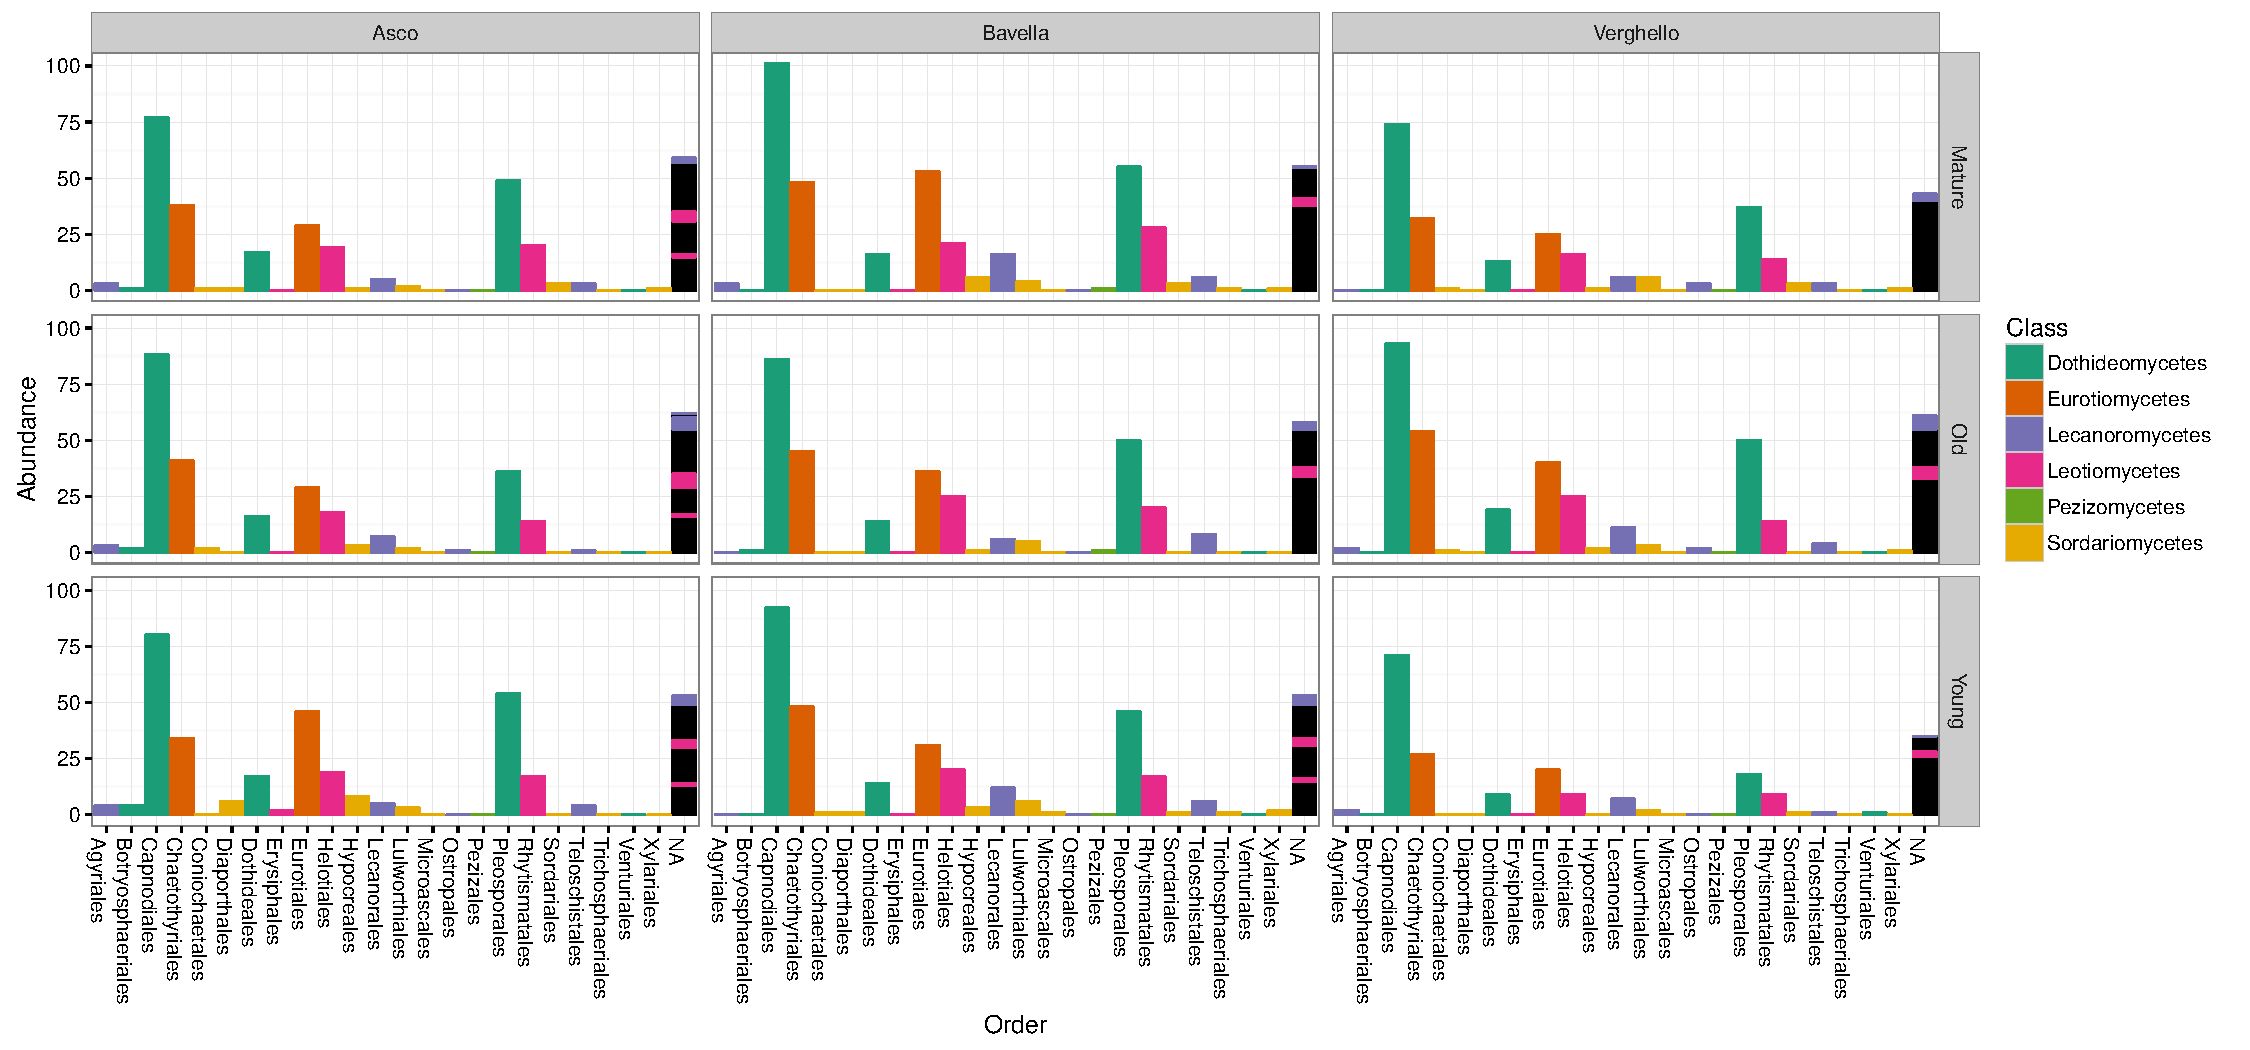
\includegraphics[width=\maxwidth]{figure/unnamed-chunk-67-1} 

}

\caption[Taxonomic distribution of OTUs in the different site * age combinaison]{Taxonomic distribution of OTUs in the different site * age combinaison.}\label{fig:unnamed-chunk-67}
\end{figure}


\end{knitrout}
\end{landscape}


  \subsection{Differences in abundances for each OTUs}
    \subsubsection{Pairwise comparison of the OTUs composition by sites}

\begin{knitrout}\small
\definecolor{shadecolor}{rgb}{0.969, 0.969, 0.969}\color{fgcolor}\begin{kframe}
\begin{alltt}
\hlkwd{library}\hlstd{(}\hlstr{"DESeq2"}\hlstd{)}
\hlkwd{packageVersion}\hlstd{(}\hlstr{"DESeq2"}\hlstd{)}
\end{alltt}
\begin{verbatim}
## [1] '1.12.3'
\end{verbatim}
\begin{alltt}
\hlstd{data.f3_deseq2} \hlkwb{<-} \hlkwd{phyloseq_to_deseq2}\hlstd{(data.f3,} \hlopt{~} \hlstd{Sites)}
\hlstd{data.f3_deseq2} \hlkwb{<-} \hlkwd{DESeq}\hlstd{(data.f3_deseq2,} \hlkwc{test} \hlstd{=} \hlstr{"Wald"}\hlstd{,} \hlkwc{fitType} \hlstd{=} \hlstr{"parametric"}\hlstd{)}
\hlstd{res.f3_deseq2} \hlkwb{<-} \hlkwd{results}\hlstd{(data.f3_deseq2)}
\end{alltt}
\end{kframe}
\end{knitrout}

\begin{knitrout}\small
\definecolor{shadecolor}{rgb}{0.969, 0.969, 0.969}\color{fgcolor}\begin{kframe}
\begin{alltt}
\hlstd{res_VA} \hlkwb{<-} \hlkwd{plot_deseq2_phyloseq}\hlstd{(data.f3_deseq2,} \hlkwc{tax_table} \hlstd{= data.f3}\hlopt{@}\hlkwc{tax_table}\hlstd{,}
                               \hlkwc{contrast} \hlstd{=} \hlkwd{c}\hlstd{(}\hlstr{"Sites"}\hlstd{,} \hlstr{"Verghello"}\hlstd{,} \hlstr{"Asco"}\hlstd{),}
                               \hlkwc{taxa} \hlstd{=} \hlstr{"Species"}\hlstd{,} \hlkwc{color_tax} \hlstd{=} \hlstr{"Class"}\hlstd{)}
\hlstd{res_VA}
\end{alltt}
\end{kframe}\begin{figure}

{\centering 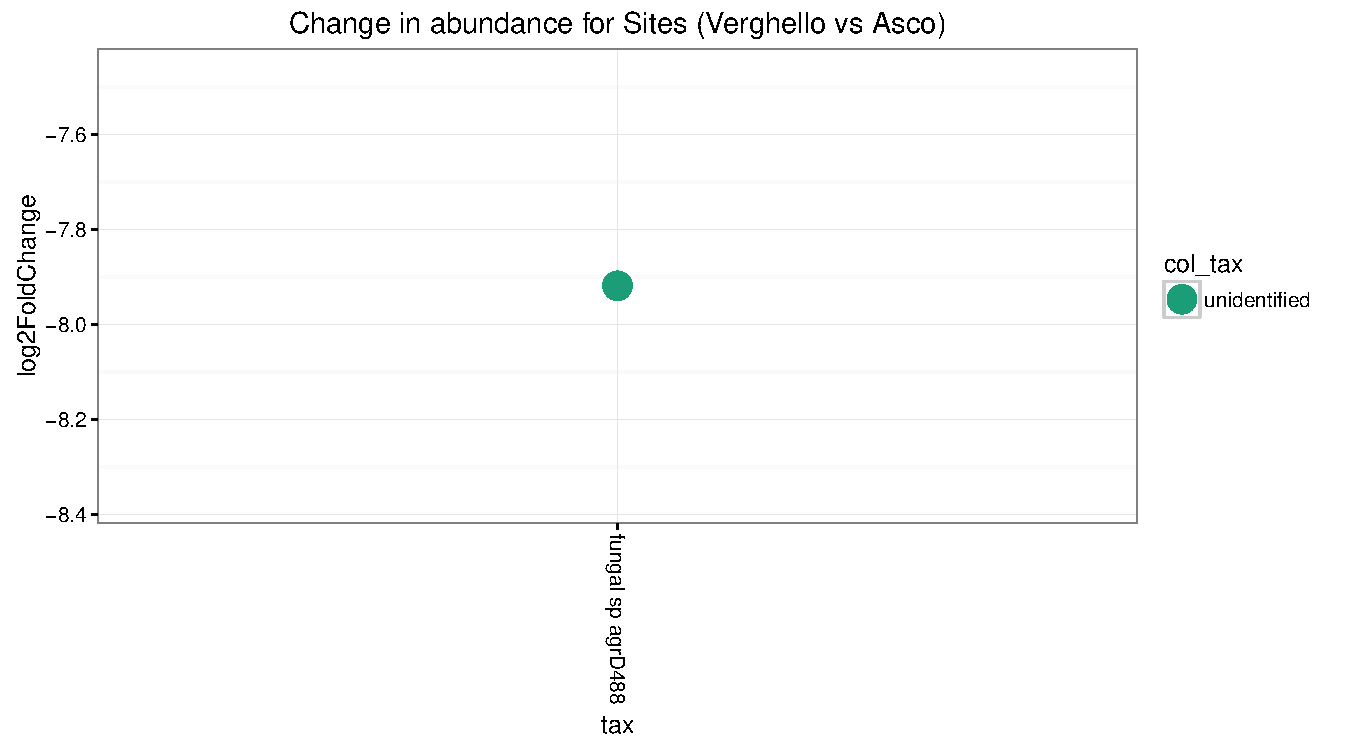
\includegraphics[width=\maxwidth]{figure/unnamed-chunk-69-1} 

}

\caption[OTUs significantly different in terms of abundances between Verghello (positive values) and Asco (negative values)]{OTUs significantly different in terms of abundances between Verghello (positive values) and Asco (negative values)}\label{fig:unnamed-chunk-69}
\end{figure}


\end{knitrout}

\begin{knitrout}\small
\definecolor{shadecolor}{rgb}{0.969, 0.969, 0.969}\color{fgcolor}\begin{kframe}
\begin{alltt}
\hlstd{res_VB} \hlkwb{<-} \hlkwd{plot_deseq2_phyloseq}\hlstd{(data.f3_deseq2,} \hlkwc{tax_table} \hlstd{= data.f3}\hlopt{@}\hlkwc{tax_table}\hlstd{,}
                               \hlkwc{contrast} \hlstd{=} \hlkwd{c}\hlstd{(}\hlstr{"Sites"}\hlstd{,} \hlstr{"Verghello"}\hlstd{,} \hlstr{"Bavella"}\hlstd{),}
                               \hlkwc{taxa} \hlstd{=} \hlstr{"Species"}\hlstd{,} \hlkwc{color_tax} \hlstd{=} \hlstr{"Class"}\hlstd{)}
\hlstd{res_VB}
\end{alltt}
\end{kframe}\begin{figure}

{\centering 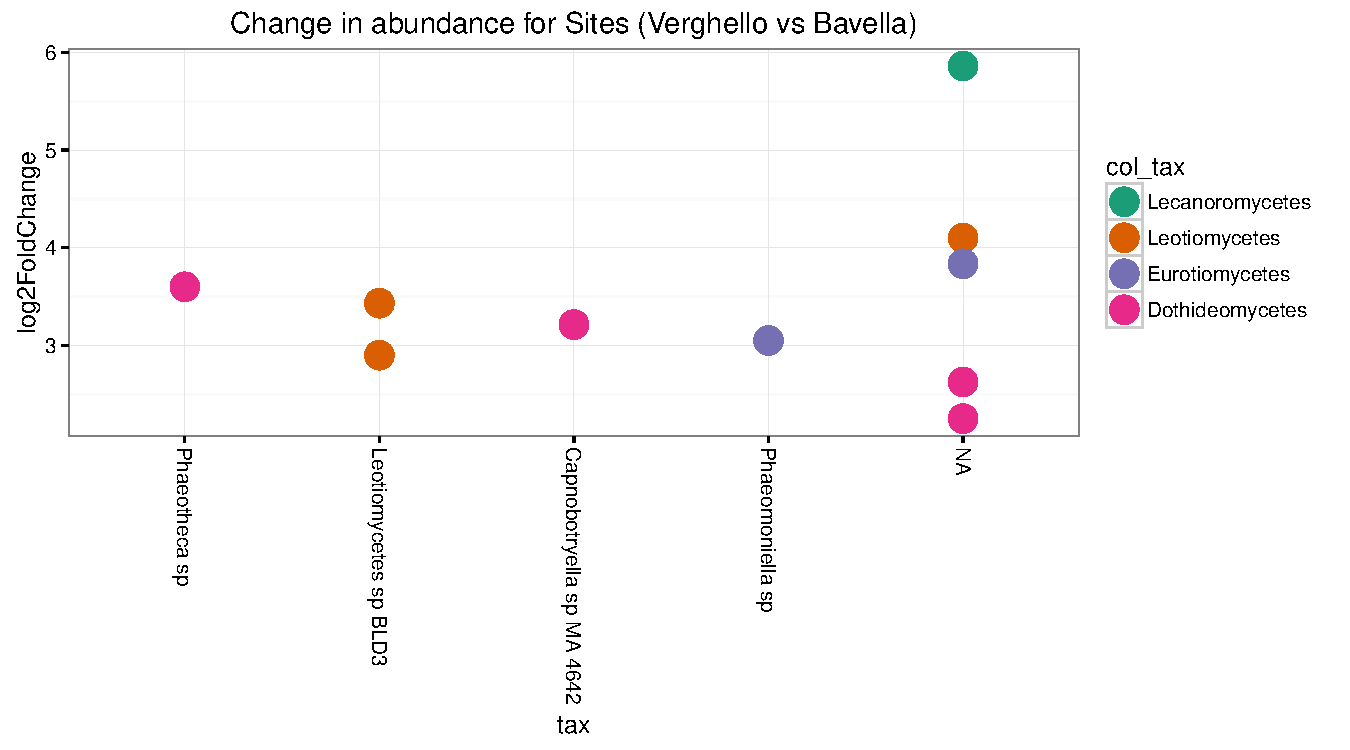
\includegraphics[width=\maxwidth]{figure/unnamed-chunk-70-1} 

}

\caption[OTUs significantly different in terms of abundances between Verghello (positive values) and Bavella (negative values)]{OTUs significantly different in terms of abundances between Verghello (positive values) and Bavella (negative values)}\label{fig:unnamed-chunk-70}
\end{figure}


\end{knitrout}

\begin{landscape}
\begin{knitrout}\small
\definecolor{shadecolor}{rgb}{0.969, 0.969, 0.969}\color{fgcolor}\begin{kframe}
\begin{alltt}
\hlstd{res_AB} \hlkwb{<-} \hlkwd{plot_deseq2_phyloseq}\hlstd{(data.f3_deseq2,} \hlkwc{tax_table} \hlstd{= data.f3}\hlopt{@}\hlkwc{tax_table}\hlstd{,}
                               \hlkwc{contrast} \hlstd{=} \hlkwd{c}\hlstd{(}\hlstr{"Sites"}\hlstd{,} \hlstr{"Asco"}\hlstd{,} \hlstr{"Bavella"}\hlstd{),}
                               \hlkwc{taxa} \hlstd{=} \hlstr{"Species"}\hlstd{,} \hlkwc{color_tax} \hlstd{=} \hlstr{"Class"}\hlstd{)}
\hlstd{res_AB}
\end{alltt}
\end{kframe}\begin{figure}

{\centering 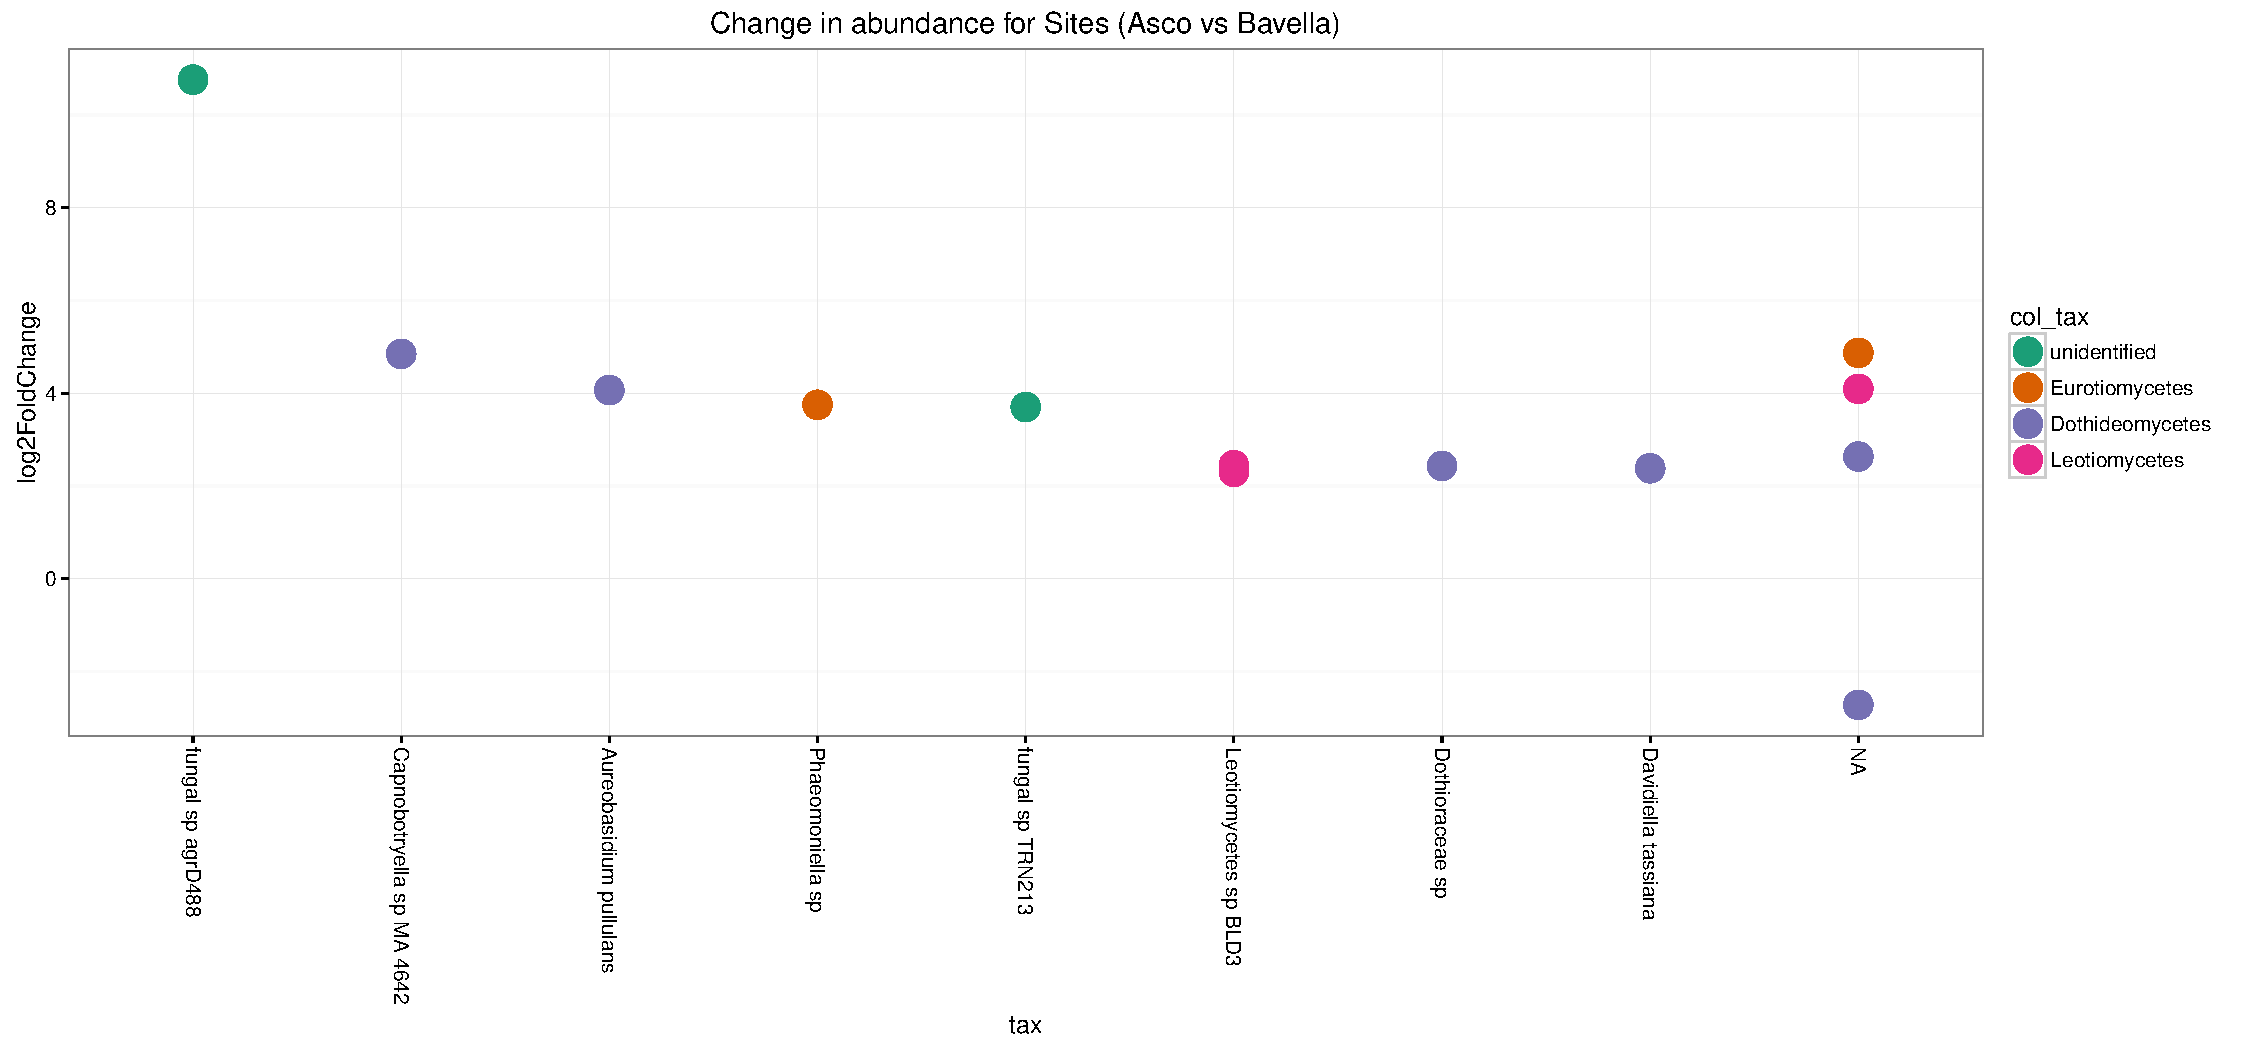
\includegraphics[width=\maxwidth]{figure/unnamed-chunk-71-1} 

}

\caption[OTUs significantly different in terms of abundances between Asco (positive values) and Bavella (negative values)]{OTUs significantly different in terms of abundances between Asco (positive values) and Bavella (negative values)}\label{fig:unnamed-chunk-71}
\end{figure}


\end{knitrout}
\end{landscape}

% latex table generated in R 3.3.1 by xtable 1.8-2 package
% Tue Jul 19 18:58:57 2016
\begin{table}[ht]
\centering
\begingroup\tiny
\begin{tabular}{lllll}
  \hline
 & Comparison & Species & Class & log2FoldChange 
 (negative = more on second levels) \\ 
  \hline
1 & Verghello vs Asco &  &  & -3.77841397359728 \\ 
  2 & Verghello vs Asco & Davidiella tassiana & Dothideomycetes & -2.3292426554423 \\ 
  3 & Verghello vs Asco &  & Dothideomycetes & -3.61893267806188 \\ 
  4 & Verghello vs Asco & fungal sp TRN213 & unidentified & -3.13867374480923 \\ 
  5 & Verghello vs Asco &  & Dothideomycetes & -3.75809969070393 \\ 
  6 & Verghello vs Asco & Capnobotryella sp MA 4642 & Dothideomycetes & -2.28440906171705 \\ 
  7 & Verghello vs Asco &  &  & -3.39552445859464 \\ 
  8 & Verghello vs Asco &  &  & -2.45061056468389 \\ 
  9 & Verghello vs Asco &  & Dothideomycetes & -2.93876057054674 \\ 
  10 & Verghello vs Asco &  &  & -2.1231609092589 \\ 
  11 & Verghello vs Asco &  &  & -2.21785279122499 \\ 
  12 & Verghello vs Asco &  &  & 3.27030586093898 \\ 
  13 & Verghello vs Asco & Dothideomycetes sp 11147 & Dothideomycetes & -3.35876370715981 \\ 
  14 & Verghello vs Asco & Phaeomoniella sp & Eurotiomycetes & -3.05588415677775 \\ 
  15 & Verghello vs Asco &  &  & 2.81017146488419 \\ 
  16 & Verghello vs Asco &  & Dothideomycetes & -2.80304424723716 \\ 
  17 & Verghello vs Asco & Capnobotryella sp MA 4642 & Dothideomycetes & -2.58963016020498 \\ 
  18 & Verghello vs Asco &  &  & -2.66392724218722 \\ 
  19 & Verghello vs Asco &  & Leotiomycetes & -3.21880600708015 \\ 
  20 & Verghello vs Asco &  &  & 2.92930724447245 \\ 
  21 & Verghello vs Asco &  & Leotiomycetes & -1.91162202262244 \\ 
  22 & Verghello vs Asco & fungal sp TRN287 & unidentified & -3.26119286517465 \\ 
  23 & Verghello vs Asco &  & Dothideomycetes & -3.73051774614064 \\ 
  24 & Verghello vs Asco &  & Dothideomycetes & -3.59888389077174 \\ 
  25 & Verghello vs Asco &  &  & -2.83113825848711 \\ 
  26 & Verghello vs Asco &  & Dothideomycetes & -2.5879763123238 \\ 
  27 & Verghello vs Asco &  &  & 3.35206655526952 \\ 
  28 & Verghello vs Asco &  & Dothideomycetes & -2.9060336204246 \\ 
  29 & Verghello vs Asco &  & Dothideomycetes & -3.67134758989312 \\ 
  30 & Verghello vs Asco & fungal sp TRN287 & unidentified & -3.50648758643916 \\ 
  31 & Verghello vs Asco &  &  & 3.49214798503904 \\ 
  32 & Verghello vs Asco &  &  & -4.04018643085912 \\ 
  33 & Verghello vs Asco &  & Dothideomycetes & -2.81488163023687 \\ 
  34 & Verghello vs Asco & Phaeotheca sp & Dothideomycetes & -3.91229888934689 \\ 
  35 & Verghello vs Asco &  & Dothideomycetes & -7.29191587441624 \\ 
  36 & Verghello vs Asco &  &  & 3.23002020397034 \\ 
  37 & Verghello vs Asco & Capnobotryella sp MA 4642 & Dothideomycetes & -2.63737112217892 \\ 
  38 & Verghello vs Asco &  &  & -2.50206160823865 \\ 
  39 & Verghello vs Asco &  &  & -2.82304112819981 \\ 
  40 & Verghello vs Asco &  & Dothideomycetes & -3.27632848840878 \\ 
  41 & Verghello vs Asco &  & Dothideomycetes & -2.85862844695998 \\ 
  42 & Verghello vs Asco &  & Dothideomycetes & -3.07243778803445 \\ 
  43 & Verghello vs Asco & Capnobotryella sp MA 4642 & Dothideomycetes & -2.52643633508039 \\ 
  44 & Verghello vs Asco &  &  & -3.39957820725733 \\ 
  45 & Verghello vs Asco & Rhytismatales sp & Leotiomycetes & -4.41293144741018 \\ 
  46 & Verghello vs Asco & Lachnellula calyciformis & Leotiomycetes & -4.09918269948416 \\ 
  47 & Verghello vs Asco & fungal sp agrD488 & unidentified & -6.69748501563904 \\ 
  48 & Verghello vs Asco &  & Dothideomycetes & -3.52986856375373 \\ 
  49 & Verghello vs Asco & Capnobotryella sp MA 4642 & Dothideomycetes & -3.02821213013443 \\ 
  50 & Verghello vs Asco & fungal sp agrD488 & unidentified & -4.57678613187943 \\ 
  51 & Verghello vs Asco &  &  & -4.70934332226896 \\ 
  52 & Verghello vs Asco & fungal sp TRN287 & unidentified & -3.33131311490098 \\ 
  53 & Verghello vs Asco & Capnobotryella sp MA 4642 & Dothideomycetes & -3.12702893768946 \\ 
  54 & Verghello vs Asco &  & Dothideomycetes & -2.8017685199665 \\ 
  55 & Verghello vs Asco &  &  & -10.6184764534919 \\ 
  56 & Verghello vs Asco & Lophodermium seditiosum & Leotiomycetes & 2.46708644436988 \\ 
  57 & Verghello vs Asco & Phaeotheca sp & Dothideomycetes & 2.74556852483771 \\ 
  58 & Verghello vs Asco &  &  & 3.33735059573991 \\ 
  59 & Verghello vs Asco &  &  & 3.33852254374311 \\ 
  60 & Verghello vs Asco &  & Dothideomycetes & -3.59877394044465 \\ 
  61 & Verghello vs Asco &  & Dothideomycetes & -2.81574973844836 \\ 
  62 & Verghello vs Asco &  & Dothideomycetes & -5.31880689803234 \\ 
  63 & Verghello vs Asco & Sarea sp & Lecanoromycetes & 5.35004486549744 \\ 
  64 & Verghello vs Asco & Sporormiaceae sp & Dothideomycetes & -5.27566358814124 \\ 
  65 & Verghello vs Asco &  & Dothideomycetes & -3.88846863260061 \\ 
  66 & Verghello vs Asco &  &  & 5.97869844874395 \\ 
  67 & Verghello vs Bavella & Phaeomoniella sp & Eurotiomycetes & 2.92820119286806 \\ 
  68 & Verghello vs Bavella &  & Dothideomycetes & 1.84664832298385 \\ 
  69 & Verghello vs Bavella & Lophodermium conigenum & Leotiomycetes & 3.87776049046955 \\ 
  70 & Verghello vs Bavella & fungal sp TRN287 & unidentified & 2.73394822182892 \\ 
  71 & Verghello vs Bavella & Capnobotryella sp MA 4642 & Dothideomycetes & 2.46470174560228 \\ 
  72 & Verghello vs Bavella &  & Dothideomycetes & 2.69029588324704 \\ 
  73 & Verghello vs Bavella & Leotiomycetes sp BLD3 & Leotiomycetes & 3.79199439132598 \\ 
  74 & Verghello vs Bavella &  & Dothideomycetes & 2.50907147594031 \\ 
  75 & Verghello vs Bavella &  &  & 3.67527127660293 \\ 
  76 & Verghello vs Bavella &  & Leotiomycetes & 3.90411109963067 \\ 
  77 & Verghello vs Bavella &  & Leotiomycetes & 3.76540742038509 \\ 
  78 & Verghello vs Bavella &  &  & 5.28089742779245 \\ 
  79 & Verghello vs Bavella & Dothioraceae sp & Dothideomycetes & 2.427402858263 \\ 
  80 & Verghello vs Bavella & Phaeotheca sp & Dothideomycetes & 5.00286308261026 \\ 
  81 & Verghello vs Bavella &  &  & 2.99842985863806 \\ 
  82 & Verghello vs Bavella &  & Dothideomycetes & 2.14743129703637 \\ 
  83 & Verghello vs Bavella & Lophodermium conigenum & Leotiomycetes & 3.93203634659419 \\ 
  84 & Verghello vs Bavella &  & Dothideomycetes & 2.16772856631734 \\ 
  85 & Verghello vs Bavella & fungal sp TRN287 & unidentified & 3.03439420023129 \\ 
  86 & Verghello vs Bavella &  &  & 3.83667679584981 \\ 
  87 & Verghello vs Bavella & Ochrocladosporium sp & Dothideomycetes & 4.31719640571145 \\ 
  88 & Verghello vs Bavella &  & Leotiomycetes & 3.79823021765702 \\ 
  89 & Verghello vs Bavella &  & Leotiomycetes & 4.29395140158755 \\ 
  90 & Verghello vs Bavella &  & Leotiomycetes & 2.29421242892866 \\ 
  91 & Verghello vs Bavella &  &  & 6.5282066602472 \\ 
  92 & Verghello vs Bavella &  & Dothideomycetes & -2.54157337757549 \\ 
  93 & Verghello vs Bavella & Leotiomycetes sp BLD3 & Leotiomycetes & 3.22490791523471 \\ 
  94 & Verghello vs Bavella & Ochrocladosporium sp & Dothideomycetes & 4.46718046676545 \\ 
  95 & Verghello vs Bavella & Knufia sp & Incertae sedis & 2.98153304536828 \\ 
  96 & Verghello vs Bavella & Capnobotryella sp MA 4642 & Dothideomycetes & 2.55071581339411 \\ 
  97 & Verghello vs Bavella &  & Dothideomycetes & 2.37437393788857 \\ 
  98 & Verghello vs Bavella &  & Leotiomycetes & 1.70475613364684 \\ 
  99 & Verghello vs Bavella &  &  & 4.61896240859855 \\ 
  100 & Verghello vs Bavella & fungal sp TRN287 & unidentified & 3.9512454264957 \\ 
  101 & Verghello vs Bavella &  & Dothideomycetes & 3.35449916658489 \\ 
  102 & Verghello vs Bavella & Lophodermium conigenum & Leotiomycetes & 3.20990352420892 \\ 
  103 & Verghello vs Bavella &  & Leotiomycetes & 2.01227003493554 \\ 
  104 & Verghello vs Bavella &  & Dothideomycetes & 2.18720673517677 \\ 
  105 & Verghello vs Bavella &  & Dothideomycetes & 2.55080984617743 \\ 
  106 & Verghello vs Bavella &  &  & 4.94778862092973 \\ 
  107 & Verghello vs Bavella &  & Leotiomycetes & 3.02457651202801 \\ 
  108 & Verghello vs Bavella &  &  & 3.340708383846 \\ 
  109 & Verghello vs Bavella & Dothioraceae sp & Dothideomycetes & 3.34578606312939 \\ 
  110 & Verghello vs Bavella &  & Leotiomycetes & 3.07464769101803 \\ 
  111 & Verghello vs Bavella &  & Leotiomycetes & 4.41566641999886 \\ 
  112 & Verghello vs Bavella &  &  & 7.04676131586348 \\ 
  113 & Verghello vs Bavella &  &  & 3.51737660246341 \\ 
  114 & Verghello vs Bavella & Dothioraceae sp & Dothideomycetes & 2.31504516154415 \\ 
  115 & Verghello vs Bavella &  & Leotiomycetes & 4.40510808121322 \\ 
  116 & Verghello vs Bavella & Dothioraceae sp & Dothideomycetes & 2.53374813917492 \\ 
  117 & Verghello vs Bavella &  &  & 4.01264160413998 \\ 
  118 & Verghello vs Bavella & Lophodermium conigenum & Leotiomycetes & 2.20086652218311 \\ 
  119 & Verghello vs Bavella &  & Leotiomycetes & 3.39185349497254 \\ 
  120 & Verghello vs Bavella &  & Leotiomycetes & 2.92410996766132 \\ 
  121 & Verghello vs Bavella &  & Leotiomycetes & 3.63747400668272 \\ 
  122 & Verghello vs Bavella &  &  & 3.72562854278191 \\ 
  123 & Verghello vs Bavella &  & Dothideomycetes & 1.97252025089449 \\ 
  124 & Verghello vs Bavella &  &  & 3.42446784460426 \\ 
  125 & Verghello vs Bavella & Ochrocladosporium sp & Dothideomycetes & 2.86141878797024 \\ 
  126 & Verghello vs Bavella &  & Leotiomycetes & 2.73706525818217 \\ 
  127 & Verghello vs Bavella & Phaeomoniella sp & Eurotiomycetes & 3.5267372523156 \\ 
  128 & Verghello vs Bavella & Leotiomycetes sp BLD3 & Leotiomycetes & 2.95865363280525 \\ 
  129 & Verghello vs Bavella &  & Leotiomycetes & 3.86154180579769 \\ 
  130 & Verghello vs Bavella &  &  & 4.28215533118863 \\ 
  131 & Verghello vs Bavella &  & Dothideomycetes & 1.8698822201162 \\ 
  132 & Verghello vs Bavella & Cyclaneusma minus & Leotiomycetes & 2.10406785933651 \\ 
  133 & Verghello vs Bavella &  & Leotiomycetes & 2.98414758469743 \\ 
  134 & Verghello vs Bavella &  &  & 3.78427843685153 \\ 
  135 & Verghello vs Bavella & Leotiomycetes sp BLD3 & Leotiomycetes & 3.10771098828849 \\ 
  136 & Verghello vs Bavella &  & Leotiomycetes & 3.44709942894777 \\ 
  137 & Verghello vs Bavella &  & Leotiomycetes & 3.02059463289777 \\ 
  138 & Verghello vs Bavella &  & Dothideomycetes & -2.95851251965281 \\ 
  139 & Verghello vs Bavella &  & Leotiomycetes & 3.73083456508718 \\ 
  140 & Verghello vs Bavella &  &  & 3.27316025243198 \\ 
  141 & Verghello vs Bavella & Leotiomycetes sp BLD3 & Leotiomycetes & 2.70802967708667 \\ 
  142 & Verghello vs Bavella &  & Leotiomycetes & 3.87460653519902 \\ 
  143 & Verghello vs Bavella & Phaeothecoidea sp & Dothideomycetes & 2.73563211068891 \\ 
  144 & Verghello vs Bavella &  & Dothideomycetes & -2.81391628257566 \\ 
  145 & Verghello vs Bavella &  & Leotiomycetes & 3.10538085333592 \\ 
  146 & Verghello vs Bavella &  &  & 5.65027793326634 \\ 
  147 & Verghello vs Bavella &  & Leotiomycetes & 3.38268263730941 \\ 
  148 & Verghello vs Bavella & Ochrocladosporium sp & Dothideomycetes & 4.65477891471599 \\ 
  149 & Verghello vs Bavella &  &  & 3.20400995702018 \\ 
  150 & Verghello vs Bavella &  & Eurotiomycetes & 3.44081828551393 \\ 
  151 & Verghello vs Bavella & Lophodermium conigenum & Leotiomycetes & 4.18334280236209 \\ 
  152 & Verghello vs Bavella &  &  & 3.8175200349921 \\ 
  153 & Verghello vs Bavella &  & Leotiomycetes & 4.0956075715652 \\ 
  154 & Verghello vs Bavella & Phaeotheca sp & Dothideomycetes & 3.60814695922571 \\ 
  155 & Verghello vs Bavella &  & Leotiomycetes & 3.15946828779453 \\ 
  156 & Verghello vs Bavella &  &  & 4.01809139801712 \\ 
  157 & Verghello vs Bavella & Leotiomycetes sp BLD3 & Leotiomycetes & 2.63396302520082 \\ 
  158 & Verghello vs Bavella &  & Leotiomycetes & 2.99742901591866 \\ 
  159 & Verghello vs Bavella &  &  & 3.05440566852503 \\ 
  160 & Verghello vs Bavella &  &  & 6.25582298963432 \\ 
  161 & Verghello vs Bavella &  &  & 3.53936821810962 \\ 
  162 & Verghello vs Bavella &  &  & 3.10630613247396 \\ 
  163 & Verghello vs Bavella &  & Leotiomycetes & 2.81932648435001 \\ 
  164 & Verghello vs Bavella &  & Leotiomycetes & 3.33842832019887 \\ 
  165 & Verghello vs Bavella &  &  & 3.90534108322187 \\ 
  166 & Verghello vs Bavella &  &  & 3.42726805069866 \\ 
  167 & Verghello vs Bavella &  &  & 3.50754673201299 \\ 
  168 & Verghello vs Bavella &  & Leotiomycetes & 1.87088301774728 \\ 
  169 & Verghello vs Bavella &  &  & 3.53341853509739 \\ 
  170 & Verghello vs Bavella &  & Leotiomycetes & 2.78773948532351 \\ 
  171 & Verghello vs Bavella & Lophodermium conigenum & Leotiomycetes & 3.65500796009109 \\ 
  172 & Verghello vs Bavella & Leotiomycetes sp BLD3 & Leotiomycetes & 2.89373217193017 \\ 
  173 & Verghello vs Bavella & Ochrocladosporium sp & Dothideomycetes & 4.0957913057351 \\ 
  174 & Verghello vs Bavella &  &  & 4.76689023724607 \\ 
  175 & Verghello vs Bavella &  & Leotiomycetes & 3.27786397150953 \\ 
  176 & Verghello vs Bavella & Leotiomycetes sp BLD3 & Leotiomycetes & 3.04839962965472 \\ 
  177 & Verghello vs Bavella &  & Leotiomycetes & 2.46418499311021 \\ 
  178 & Verghello vs Bavella & Leotiomycetes sp BLD3 & Leotiomycetes & 2.65835054550231 \\ 
  179 & Verghello vs Bavella &  &  & 4.42896907079518 \\ 
  180 & Verghello vs Bavella &  &  & 4.86795018194018 \\ 
  181 & Verghello vs Bavella &  &  & 2.88286940700648 \\ 
  182 & Verghello vs Bavella &  & Leotiomycetes & 3.28024540085685 \\ 
  183 & Verghello vs Bavella & Aureobasidium pullulans & Dothideomycetes & 3.76787010946416 \\ 
  184 & Verghello vs Bavella & Phaeotheca sp & Dothideomycetes & 3.19092674233036 \\ 
  185 & Verghello vs Bavella &  & Leotiomycetes & 3.48356934658702 \\ 
  186 & Verghello vs Bavella &  & Leotiomycetes & 4.35289016747672 \\ 
  187 & Verghello vs Bavella & Dothioraceae sp & Dothideomycetes & 2.7405385725021 \\ 
  188 & Verghello vs Bavella &  & Leotiomycetes & 2.23509800428021 \\ 
  189 & Verghello vs Bavella &  & Dothideomycetes & -2.13431564363241 \\ 
  190 & Verghello vs Bavella &  & Leotiomycetes & 2.98531614170849 \\ 
  191 & Verghello vs Bavella &  & Leotiomycetes & 3.98844677972022 \\ 
  192 & Verghello vs Bavella & Lophodermium conigenum & Leotiomycetes & 2.50079917943419 \\ 
  193 & Verghello vs Bavella &  & Leotiomycetes & 2.74129717197842 \\ 
  194 & Verghello vs Bavella &  & Leotiomycetes & 3.72122827781254 \\ 
  195 & Verghello vs Bavella &  & Leotiomycetes & 3.48536891305845 \\ 
  196 & Verghello vs Bavella & Ochrocladosporium sp & Dothideomycetes & 2.49259177688475 \\ 
  197 & Verghello vs Bavella &  &  & 4.11155551072933 \\ 
  198 & Verghello vs Bavella &  &  & 5.55382954797365 \\ 
  199 & Verghello vs Bavella &  & Dothideomycetes & -2.34083109365925 \\ 
  200 & Verghello vs Bavella & Lachnellula calyciformis & Leotiomycetes & -3.21362822482304 \\ 
  201 & Verghello vs Bavella &  &  & 5.57422986271078 \\ 
  202 & Verghello vs Bavella &  &  & 4.55202819335804 \\ 
  203 & Verghello vs Bavella &  &  & 2.83238903785241 \\ 
  204 & Verghello vs Bavella &  & Lecanoromycetes & 6.48831431684019 \\ 
  205 & Asco vs Bavella & Phaeomoniella sp & Eurotiomycetes & 3.09287718947601 \\ 
  206 & Asco vs Bavella &  & Dothideomycetes & 2.62287741837029 \\ 
  207 & Asco vs Bavella & Cryptodiscus microstomus & Lecanoromycetes & 4.00286262408016 \\ 
  208 & Asco vs Bavella & Lophodermium conigenum & Leotiomycetes & 4.27731904569942 \\ 
  209 & Asco vs Bavella & fungal sp TRN287 & unidentified & 4.97568244367431 \\ 
  210 & Asco vs Bavella &  &  & 3.87301189469536 \\ 
  211 & Asco vs Bavella & Capnobotryella sp MA 4642 & Dothideomycetes & 4.88431558546374 \\ 
  212 & Asco vs Bavella & Leotiomycetes sp BLD3 & Leotiomycetes & 3.18955519564381 \\ 
  213 & Asco vs Bavella &  & Dothideomycetes & 2.92677835808822 \\ 
  214 & Asco vs Bavella &  &  & 4.21050292270625 \\ 
  215 & Asco vs Bavella &  & Leotiomycetes & 4.37849719722896 \\ 
  216 & Asco vs Bavella &  & Leotiomycetes & 4.42318874087787 \\ 
  217 & Asco vs Bavella &  &  & 7.21562713292429 \\ 
  218 & Asco vs Bavella & Dothioraceae sp & Dothideomycetes & 3.03956106582894 \\ 
  219 & Asco vs Bavella & Phaeotheca sp & Dothideomycetes & 7.13942539693825 \\ 
  220 & Asco vs Bavella &  & Dothideomycetes & 2.61502738649308 \\ 
  221 & Asco vs Bavella & Lophodermium conigenum & Leotiomycetes & 4.56821380333654 \\ 
  222 & Asco vs Bavella &  & Dothideomycetes & 2.13608251016564 \\ 
  223 & Asco vs Bavella & fungal sp TRN287 & unidentified & 5.21316734315387 \\ 
  224 & Asco vs Bavella &  &  & 4.89330320616051 \\ 
  225 & Asco vs Bavella & Ochrocladosporium sp & Dothideomycetes & 2.99347143389959 \\ 
  226 & Asco vs Bavella & Davidiella tassiana & Dothideomycetes & 2.58088528668437 \\ 
  227 & Asco vs Bavella &  & Leotiomycetes & 4.0688213410021 \\ 
  228 & Asco vs Bavella &  & Leotiomycetes & 4.31151931662068 \\ 
  229 & Asco vs Bavella & Phaeomoniella sp & Eurotiomycetes & 1.68445661118026 \\ 
  230 & Asco vs Bavella & fungal sp TRN213 & unidentified & 6.38717794858472 \\ 
  231 & Asco vs Bavella &  & Dothideomycetes & 5.7022136874769 \\ 
  232 & Asco vs Bavella & Capnobotryella sp MA 4642 & Dothideomycetes & 2.74474674734007 \\ 
  233 & Asco vs Bavella & fungal sp TRN213 & unidentified & 3.67480705130822 \\ 
  234 & Asco vs Bavella &  & Leotiomycetes & 2.74556302740686 \\ 
  235 & Asco vs Bavella & fungal sp TRN213 & unidentified & 3.93037693564207 \\ 
  236 & Asco vs Bavella &  &  & 3.64688458024233 \\ 
  237 & Asco vs Bavella &  & Dothideomycetes & 2.21616083507448 \\ 
  238 & Asco vs Bavella & Phaeomoniella sp & Eurotiomycetes & 3.40257796308151 \\ 
  239 & Asco vs Bavella &  & Dothideomycetes & 3.51867880930368 \\ 
  240 & Asco vs Bavella & Leotiomycetes sp BLD3 & Leotiomycetes & 2.45734263964316 \\ 
  241 & Asco vs Bavella & Knufia sp & Incertae sedis & 3.28546090536058 \\ 
  242 & Asco vs Bavella &  & Dothideomycetes & 2.45127345220028 \\ 
  243 & Asco vs Bavella & Capnobotryella sp MA 4642 & Dothideomycetes & 4.83512487511117 \\ 
  244 & Asco vs Bavella &  &  & 6.01962024394053 \\ 
  245 & Asco vs Bavella &  & Dothideomycetes & 2.07387398590573 \\ 
  246 & Asco vs Bavella &  & Leotiomycetes & 1.87080443954534 \\ 
  247 & Asco vs Bavella &  &  & 7.06957297328244 \\ 
  248 & Asco vs Bavella & fungal sp TRN287 & unidentified & 4.06980863383354 \\ 
  249 & Asco vs Bavella &  & Dothideomycetes & 2.69795676635064 \\ 
  250 & Asco vs Bavella & Lophodermium conigenum & Leotiomycetes & 3.72995599415389 \\ 
  251 & Asco vs Bavella &  & Dothideomycetes & 2.98496201297709 \\ 
  252 & Asco vs Bavella &  & Leotiomycetes & 1.9699249716172 \\ 
  253 & Asco vs Bavella &  & Dothideomycetes & 2.75043931214593 \\ 
  254 & Asco vs Bavella &  &  & 7.07094953018863 \\ 
  255 & Asco vs Bavella &  & Leotiomycetes & 3.12503354468158 \\ 
  256 & Asco vs Bavella &  &  & 5.558561175071 \\ 
  257 & Asco vs Bavella & Dothioraceae sp & Dothideomycetes & 3.37170330705796 \\ 
  258 & Asco vs Bavella & fungal sp TRN287 & unidentified & 3.00976852549683 \\ 
  259 & Asco vs Bavella &  & Leotiomycetes & 3.60619050507127 \\ 
  260 & Asco vs Bavella &  & Leotiomycetes & 4.65188905222497 \\ 
  261 & Asco vs Bavella &  &  & 3.7764554549245 \\ 
  262 & Asco vs Bavella & Dothideomycetes sp 11147 & Dothideomycetes & 3.62298911168836 \\ 
  263 & Asco vs Bavella & Dothioraceae sp & Dothideomycetes & 2.33046314909653 \\ 
  264 & Asco vs Bavella &  & Leotiomycetes & 3.70697546111347 \\ 
  265 & Asco vs Bavella & fungal sp TRN287 & unidentified & 2.33564536487758 \\ 
  266 & Asco vs Bavella & Capnobotryella sp MA 4642 & Dothideomycetes & 3.89510233019482 \\ 
  267 & Asco vs Bavella & Phaeomoniella sp & Eurotiomycetes & 2.91479485759596 \\ 
  268 & Asco vs Bavella & Dothioraceae sp & Dothideomycetes & 2.42677717151283 \\ 
  269 & Asco vs Bavella & Phaeothecoidea sp & Dothideomycetes & -2.32888527117018 \\ 
  270 & Asco vs Bavella &  & Dothideomycetes & 4.85336317624841 \\ 
  271 & Asco vs Bavella & Lophodermium conigenum & Leotiomycetes & 2.12022219134513 \\ 
  272 & Asco vs Bavella &  & Dothideomycetes & 3.84745646974159 \\ 
  273 & Asco vs Bavella &  & Leotiomycetes & 2.87975464829814 \\ 
  274 & Asco vs Bavella &  & Leotiomycetes & 2.95883389808023 \\ 
  275 & Asco vs Bavella &  & Leotiomycetes & 2.79670358724655 \\ 
  276 & Asco vs Bavella &  & Leotiomycetes & 3.36262003915616 \\ 
  277 & Asco vs Bavella & Capnobotryella sp MA 4642 & Dothideomycetes & 4.4343610991744 \\ 
  278 & Asco vs Bavella &  & Leotiomycetes & 5.34847461412433 \\ 
  279 & Asco vs Bavella &  &  & 6.38955578496913 \\ 
  280 & Asco vs Bavella &  & Dothideomycetes & 2.15459767055099 \\ 
  281 & Asco vs Bavella &  &  & 3.77206710199984 \\ 
  282 & Asco vs Bavella &  & Leotiomycetes & 4.75932363765754 \\ 
  283 & Asco vs Bavella & Phaeomoniella sp & Eurotiomycetes & 3.06659353226047 \\ 
  284 & Asco vs Bavella & Leotiomycetes sp BLD3 & Leotiomycetes & 2.50078511005221 \\ 
  285 & Asco vs Bavella &  & Leotiomycetes & 3.71772051592413 \\ 
  286 & Asco vs Bavella & Dothideomycetes sp 11147 & Dothideomycetes & 4.11157740158376 \\ 
  287 & Asco vs Bavella &  &  & 6.55006565212544 \\ 
  288 & Asco vs Bavella &  &  & -3.4639026217573 \\ 
  289 & Asco vs Bavella &  & Leotiomycetes & 4.78052616543387 \\ 
  290 & Asco vs Bavella &  &  & -2.65447140726838 \\ 
  291 & Asco vs Bavella & fungal sp TRN287 & unidentified & 4.05590977758833 \\ 
  292 & Asco vs Bavella &  & Dothideomycetes & 2.87152261684427 \\ 
  293 & Asco vs Bavella & Capnobotryella sp MA 4642 & Dothideomycetes & 3.06103180856072 \\ 
  294 & Asco vs Bavella &  & Leotiomycetes & 3.13055583398238 \\ 
  295 & Asco vs Bavella & fungal sp TRN287 & unidentified & 4.73221167082824 \\ 
  296 & Asco vs Bavella & Capnobotryella sp MA 4642 & Dothideomycetes & 3.06347596566736 \\ 
  297 & Asco vs Bavella &  & Leotiomycetes & 3.06580269702156 \\ 
  298 & Asco vs Bavella &  & Dothideomycetes & 2.48835346415174 \\ 
  299 & Asco vs Bavella & Leotiomycetes sp BLD3 & Leotiomycetes & 2.05726433178138 \\ 
  300 & Asco vs Bavella & Dothideomycetes sp 11147 & Dothideomycetes & 3.1788725192747 \\ 
  301 & Asco vs Bavella &  & Leotiomycetes & 3.33681553430692 \\ 
  302 & Asco vs Bavella &  & Leotiomycetes & 2.54585730201249 \\ 
  303 & Asco vs Bavella & Capnobotryella sp MA 4642 & Dothideomycetes & 4.15263325012717 \\ 
  304 & Asco vs Bavella & Lophodermium conigenum & Leotiomycetes & 4.16415899485768 \\ 
  305 & Asco vs Bavella &  & Leotiomycetes & 2.77190643232398 \\ 
  306 & Asco vs Bavella &  &  & 6.10429851091909 \\ 
  307 & Asco vs Bavella & fungal sp TRN256 & unidentified & 3.66558917337731 \\ 
  308 & Asco vs Bavella & Phaeomoniella sp & Eurotiomycetes & 3.11523059677682 \\ 
  309 & Asco vs Bavella &  & Dothideomycetes & 2.47900941876533 \\ 
  310 & Asco vs Bavella & Leotiomycetes sp BLD3 & Leotiomycetes & 2.23379214376701 \\ 
  311 & Asco vs Bavella &  & Leotiomycetes & 3.95871410075849 \\ 
  312 & Asco vs Bavella & fungal sp TRN287 & unidentified & 2.80808149188312 \\ 
  313 & Asco vs Bavella &  & Leotiomycetes & 3.46247484563297 \\ 
  314 & Asco vs Bavella &  & Dothideomycetes & 2.90613130006452 \\ 
  315 & Asco vs Bavella & fungal sp TRN287 & unidentified & 3.4258999501647 \\ 
  316 & Asco vs Bavella &  & Dothideomycetes & 2.94380970234413 \\ 
  317 & Asco vs Bavella &  & Dothideomycetes & 3.0288000514432 \\ 
  318 & Asco vs Bavella & fungal sp TRN287 & unidentified & 3.97365015373498 \\ 
  319 & Asco vs Bavella &  & Leotiomycetes & 3.53956078474499 \\ 
  320 & Asco vs Bavella &  &  & 7.2441963878793 \\ 
  321 & Asco vs Bavella &  & Dothideomycetes & 4.23769228841584 \\ 
  322 & Asco vs Bavella &  & Eurotiomycetes & 5.08855432084694 \\ 
  323 & Asco vs Bavella &  & Dothideomycetes & 2.25717597014277 \\ 
  324 & Asco vs Bavella & Lophodermium conigenum & Leotiomycetes & 5.14983170647111 \\ 
  325 & Asco vs Bavella & Phaeothecoidea sp & Dothideomycetes & -2.63238724807024 \\ 
  326 & Asco vs Bavella &  &  & 3.16815415065843 \\ 
  327 & Asco vs Bavella & Dothideomycetes sp 11147 & Dothideomycetes & 3.39254810175991 \\ 
  328 & Asco vs Bavella &  & Dothideomycetes & 3.20159720448497 \\ 
  329 & Asco vs Bavella &  &  & -2.74928122249219 \\ 
  330 & Asco vs Bavella &  & Leotiomycetes & 4.10179645291239 \\ 
  331 & Asco vs Bavella & Phaeotheca sp & Dothideomycetes & 7.52044584857261 \\ 
  332 & Asco vs Bavella &  & Leotiomycetes & 3.47643740916987 \\ 
  333 & Asco vs Bavella &  & Leotiomycetes & 3.27177681546535 \\ 
  334 & Asco vs Bavella &  & Dothideomycetes & 2.05213877352598 \\ 
  335 & Asco vs Bavella &  &  & 3.18559519283251 \\ 
  336 & Asco vs Bavella & Capnobotryella sp MA 4642 & Dothideomycetes & 4.58410398819482 \\ 
  337 & Asco vs Bavella & fungal sp TRN213 & unidentified & 3.20273131693626 \\ 
  338 & Asco vs Bavella &  & Dothideomycetes & 2.27638839545122 \\ 
  339 & Asco vs Bavella &  & Dothideomycetes & 9.26472784035565 \\ 
  340 & Asco vs Bavella &  &  & 3.02580278566398 \\ 
  341 & Asco vs Bavella & Capnobotryella sp MA 4642 & Dothideomycetes & 3.77004576367367 \\ 
  342 & Asco vs Bavella & fungal sp TRN287 & unidentified & 2.90819518174916 \\ 
  343 & Asco vs Bavella & Capnobotryella sp MA 4642 & Dothideomycetes & 3.41842972375212 \\ 
  344 & Asco vs Bavella &  &  & 5.32813770535306 \\ 
  345 & Asco vs Bavella & Dothioraceae sp & Dothideomycetes & 2.43009052439774 \\ 
  346 & Asco vs Bavella & Cyclaneusma minus & Leotiomycetes & -3.19825098198894 \\ 
  347 & Asco vs Bavella & Dothioraceae sp & Dothideomycetes & 2.47272166511484 \\ 
  348 & Asco vs Bavella & Phaeomoniella sp & Eurotiomycetes & 2.93423512479059 \\ 
  349 & Asco vs Bavella &  &  & 5.48528417794664 \\ 
  350 & Asco vs Bavella &  &  & 5.92932965893731 \\ 
  351 & Asco vs Bavella &  &  & 2.72303185634701 \\ 
  352 & Asco vs Bavella &  & Dothideomycetes & -2.65082561130498 \\ 
  353 & Asco vs Bavella &  & Dothideomycetes & 3.19155649907864 \\ 
  354 & Asco vs Bavella & Capnobotryella sp MA 4642 & Dothideomycetes & 3.51079584189099 \\ 
  355 & Asco vs Bavella &  &  & 5.6632031715288 \\ 
  356 & Asco vs Bavella &  & Dothideomycetes & 3.60651911760935 \\ 
  357 & Asco vs Bavella &  & Leotiomycetes & 2.20879238084523 \\ 
  358 & Asco vs Bavella &  &  & 3.45633530259181 \\ 
  359 & Asco vs Bavella &  & Leotiomycetes & 3.30435577998993 \\ 
  360 & Asco vs Bavella &  &  & 6.31167785835021 \\ 
  361 & Asco vs Bavella &  & Dothideomycetes & 4.18734374768613 \\ 
  362 & Asco vs Bavella & Dothideomycetes sp 11147 & Dothideomycetes & 2.51516484096287 \\ 
  363 & Asco vs Bavella & Capnobotryella sp MA 4642 & Dothideomycetes & 4.4184072192147 \\ 
  364 & Asco vs Bavella & Capnobotryella sp MA 4642 & Dothideomycetes & 3.380395273301 \\ 
  365 & Asco vs Bavella &  &  & -3.35334824199256 \\ 
  366 & Asco vs Bavella & Leotiomycetes sp BLD3 & Leotiomycetes & 2.20315949686064 \\ 
  367 & Asco vs Bavella & Capnobotryella sp MA 4642 & Dothideomycetes & 3.4808525472467 \\ 
  368 & Asco vs Bavella &  &  & 4.42751724024768 \\ 
  369 & Asco vs Bavella &  &  & 4.79236366260222 \\ 
  370 & Asco vs Bavella & Rhytismatales sp & Leotiomycetes & 3.88921509322277 \\ 
  371 & Asco vs Bavella &  & Eurotiomycetes & 2.9078906769733 \\ 
  372 & Asco vs Bavella &  & Leotiomycetes & 2.7699234864231 \\ 
  373 & Asco vs Bavella &  & Dothideomycetes & 4.04417370263477 \\ 
  374 & Asco vs Bavella & fungal sp agrD488 & unidentified & 9.44089751501079 \\ 
  375 & Asco vs Bavella &  & Dothideomycetes & 2.68254192563272 \\ 
  376 & Asco vs Bavella & Capnobotryella sp MA 4642 & Dothideomycetes & 3.15134284395138 \\ 
  377 & Asco vs Bavella &  & Leotiomycetes & 3.86921924593589 \\ 
  378 & Asco vs Bavella &  & Dothideomycetes & 5.21145698711687 \\ 
  379 & Asco vs Bavella &  & Leotiomycetes & 2.7354961193296 \\ 
  380 & Asco vs Bavella & Capnobotryella sp MA 4642 & Dothideomycetes & 4.00181490305092 \\ 
  381 & Asco vs Bavella &  &  & 3.30595975796123 \\ 
  382 & Asco vs Bavella &  &  & 3.34823203995249 \\ 
  383 & Asco vs Bavella & fungal sp agrD488 & unidentified & 5.6526876882867 \\ 
  384 & Asco vs Bavella &  &  & 3.73794989455831 \\ 
  385 & Asco vs Bavella &  &  & 4.8852432940386 \\ 
  386 & Asco vs Bavella &  &  & 4.8034224365778 \\ 
  387 & Asco vs Bavella &  &  & 3.72707869703116 \\ 
  388 & Asco vs Bavella & Capnobotryella sp MA 4642 & Dothideomycetes & 3.45222996469101 \\ 
  389 & Asco vs Bavella &  & Dothideomycetes & 2.77217362733303 \\ 
  390 & Asco vs Bavella &  &  & 2.97087756149809 \\ 
  391 & Asco vs Bavella &  & Leotiomycetes & 3.79663213460952 \\ 
  392 & Asco vs Bavella &  & Dothideomycetes & 3.37723846491091 \\ 
  393 & Asco vs Bavella & Aureobasidium pullulans & Dothideomycetes & 4.16750134625602 \\ 
  394 & Asco vs Bavella & fungal sp TRN213 & unidentified & 3.17976116277508 \\ 
  395 & Asco vs Bavella &  &  & 4.27265705059644 \\ 
  396 & Asco vs Bavella &  &  & 5.79632673674507 \\ 
  397 & Asco vs Bavella & Dothioraceae sp & Dothideomycetes & -4.29226346446265 \\ 
  398 & Asco vs Bavella &  & Leotiomycetes & 3.33846582030205 \\ 
  399 & Asco vs Bavella &  & Dothideomycetes & 4.66383908875482 \\ 
  400 & Asco vs Bavella & Dothioraceae sp & Dothideomycetes & 3.83968802098568 \\ 
  401 & Asco vs Bavella & fungal sp TRN287 & unidentified & 5.21259044777175 \\ 
  402 & Asco vs Bavella &  & Leotiomycetes & 3.19945379596747 \\ 
  403 & Asco vs Bavella &  &  & -1.99473266460837 \\ 
  404 & Asco vs Bavella &  & Dothideomycetes & -1.97902813413655 \\ 
  405 & Asco vs Bavella &  &  & 3.24411510128674 \\ 
  406 & Asco vs Bavella &  & Leotiomycetes & 3.3161470166883 \\ 
  407 & Asco vs Bavella & Lophodermium conigenum & Leotiomycetes & 2.94512555175467 \\ 
  408 & Asco vs Bavella &  &  & 3.90122663848315 \\ 
  409 & Asco vs Bavella &  & Leotiomycetes & 3.12683656739652 \\ 
  410 & Asco vs Bavella & fungal sp agrD488 & unidentified & 4.57215152390053 \\ 
  411 & Asco vs Bavella & Capnobotryella sp MA 4642 & Dothideomycetes & 3.96527272544997 \\ 
  412 & Asco vs Bavella & fungal sp TRN287 & unidentified & 2.57173616767213 \\ 
  413 & Asco vs Bavella & fungal sp TRN287 & unidentified & 3.52004624694785 \\ 
  414 & Asco vs Bavella &  &  & 11.0421611970769 \\ 
  415 & Asco vs Bavella &  &  & 6.34934593051755 \\ 
  416 & Asco vs Bavella &  &  & 2.92863954763995 \\ 
  417 & Asco vs Bavella &  & Leotiomycetes & 3.4265934503702 \\ 
  418 & Asco vs Bavella &  & Leotiomycetes & 3.09867206450901 \\ 
  419 & Asco vs Bavella &  & Dothideomycetes & 2.60776086269717 \\ 
  420 & Asco vs Bavella & Lophodermium seditiosum & Leotiomycetes & -3.34050180319158 \\ 
  421 & Asco vs Bavella &  &  & 4.12286842964272 \\ 
  422 & Asco vs Bavella &  &  & 4.49524408982676 \\ 
  423 & Asco vs Bavella &  & Dothideomycetes & 3.42680481472858 \\ 
  424 & Asco vs Bavella &  &  & 3.5692938151768 \\ 
  425 & Asco vs Bavella &  & Eurotiomycetes & 4.10599312168423 \\ 
  426 & Asco vs Bavella &  &  & 6.19355966045651 \\ 
  427 & Asco vs Bavella &  & Dothideomycetes & 3.41712731188025 \\ 
  428 & Asco vs Bavella & fungal sp TRN213 & unidentified & 3.47906967041341 \\ 
  429 & Asco vs Bavella &  &  & -3.6767354237547 \\ 
  430 & Asco vs Bavella &  &  & -3.32572017110006 \\ 
  431 & Asco vs Bavella & Capnobotryella sp MA 4642 & Dothideomycetes & 3.9448658885025 \\ 
  432 & Asco vs Bavella &  & Dothideomycetes & 5.05521488743665 \\ 
  433 & Asco vs Bavella &  & Dothideomycetes & 2.82332452375886 \\ 
  434 & Asco vs Bavella & Capnobotryella sp MA 4642 & Dothideomycetes & 2.72289265006023 \\ 
  435 & Asco vs Bavella & Capnobotryella sp MA 4642 & Dothideomycetes & 4.67559743062055 \\ 
  436 & Asco vs Bavella &  & Dothideomycetes & 3.15615669507891 \\ 
  437 & Asco vs Bavella &  & Dothideomycetes & 4.28390488920998 \\ 
  438 & Asco vs Bavella &  & Dothideomycetes & 5.60292436994054 \\ 
  439 & Asco vs Bavella &  & Eurotiomycetes & 4.55708593985521 \\ 
  440 & Asco vs Bavella &  &  & 5.45359037696062 \\ 
  441 & Asco vs Bavella &  &  & 5.51323090365195 \\ 
  442 & Asco vs Bavella & Sarea sp & Lecanoromycetes & -5.21529231544417 \\ 
  443 & Asco vs Bavella &  &  & 6.4562626986662 \\ 
  444 & Asco vs Bavella &  &  & 7.02622936981689 \\ 
  445 & Asco vs Bavella & fungal sp agrD488 & unidentified & 6.2203571090961 \\ 
  446 & Asco vs Bavella &  &  & 3.88899609679248 \\ 
  447 & Asco vs Bavella &  &  & 3.33947334811414 \\ 
  448 & Asco vs Bavella &  &  & 4.65774329891391 \\ 
  449 & Asco vs Bavella &  & Dothideomycetes & 4.15782652963047 \\ 
  450 & Asco vs Bavella &  & Dothideomycetes & -1.98291494981046 \\ 
  451 & Asco vs Bavella &  & unidentified & -3.65987045702856 \\ 
   \hline
\end{tabular}
\endgroup
\caption{OTUs showing differential abundances in the different sites.} 
\end{table}


    \subsubsection{Pairwise comparison of Order composition by sites}

\begin{knitrout}\small
\definecolor{shadecolor}{rgb}{0.969, 0.969, 0.969}\color{fgcolor}\begin{kframe}
\begin{alltt}
\hlstd{res_VA_o} \hlkwb{<-} \hlkwd{plot_deseq2_phyloseq}\hlstd{(data.f3,} \hlkwc{contrast} \hlstd{=} \hlkwd{c}\hlstd{(}\hlstr{"Sites"}\hlstd{,} \hlstr{"Verghello"}\hlstd{,} \hlstr{"Asco"}\hlstd{),}
                               \hlkwc{taxDepth} \hlstd{=} \hlstr{"Order"}\hlstd{,} \hlkwc{color_tax} \hlstd{=} \hlstr{"Class"}\hlstd{)}
\hlstd{res_VB_o} \hlkwb{<-} \hlkwd{plot_deseq2_phyloseq}\hlstd{(data.f3,} \hlkwc{contrast} \hlstd{=} \hlkwd{c}\hlstd{(}\hlstr{"Sites"}\hlstd{,} \hlstr{"Verghello"}\hlstd{,} \hlstr{"Bavella"}\hlstd{),}
                               \hlkwc{taxDepth} \hlstd{=} \hlstr{"Order"}\hlstd{,} \hlkwc{color_tax} \hlstd{=} \hlstr{"Class"}\hlstd{)}
\hlstd{res_AB_o} \hlkwb{<-} \hlkwd{plot_deseq2_phyloseq}\hlstd{(data.f3,} \hlkwc{contrast} \hlstd{=} \hlkwd{c}\hlstd{(}\hlstr{"Sites"}\hlstd{,} \hlstr{"Asco"}\hlstd{,} \hlstr{"Bavella"}\hlstd{),}
                               \hlkwc{taxDepth} \hlstd{=} \hlstr{"Order"}\hlstd{,} \hlkwc{color_tax} \hlstd{=} \hlstr{"Class"}\hlstd{)}
\end{alltt}
\end{kframe}
\end{knitrout}

% latex table generated in R 3.3.1 by xtable 1.8-2 package
% Tue Jul 19 18:59:03 2016
\begin{table}[ht]
\centering
\begingroup\tiny
\begin{tabular}{lllll}
  \hline
 & Comparison & Order & Class & log2FoldChange 
 (negative = more on second levels) \\ 
  \hline
1 & Verghello vs Asco & Xylariales & Sordariomycetes & 4.2444927272089 \\ 
  2 & Verghello vs Bavella & Incertae sedis & Leotiomycetes & -1.3417319230562 \\ 
  3 & Verghello vs Bavella & unidentified & unidentified & 1.57935352182134 \\ 
  4 & Asco vs Bavella & Botryosphaeriales & Dothideomycetes & 6.05272114483586 \\ 
  5 & Asco vs Bavella & Eurotiales & Eurotiomycetes & 1.76179960851379 \\ 
  6 & Asco vs Bavella & Incertae sedis & Leotiomycetes & -1.6831940181778 \\ 
  7 & Asco vs Bavella & unidentified & unidentified & 1.44997805431064 \\ 
  8 & Asco vs Bavella & Xylariales & Sordariomycetes & -4.01099008009487 \\ 
   \hline
\end{tabular}
\endgroup
\caption{Order showing differential abundances in the different sites.} 
\end{table}


\cleardoublepage
\listoffigures
\listoftables

\end {document}

